\documentclass[authoryear]{elsarticle}

\setlength\arraycolsep{2pt}
\setlength{\parskip}{1ex plus 0.5ex minus 0.2ex}
\usepackage{graphicx}
\usepackage{amsfonts}
\usepackage{multirow}
\usepackage{comment}

%hello there
%\usepackage{chicago}
\bibliographystyle{chicago}



\newcommand{\eps}{\epsilon}
\newcommand{\var}{{\rm var}}
\newcommand{\cov}{{\rm cov}}
\newcommand{\nid}{{\rm NID}}
\newcommand{\diag}{{\rm diag}}
\newcommand{\E}{{\mathrm E}}
\newcommand{\R}{{\mathrm R}}
\newcommand{\RD}{{\tilde{\mathrm R}}}
\newcommand{\Q}{{\mathrm Q}}
\newcommand{\U}{{\mathrm U}}
\newcommand{\Ex}{{\cal E}}
\newcommand{\cor}{\mathrm{cor}}
\newcommand{\tr}{\mathrm{tr}}
\newcommand{\e}{\mathrm{e}}
\newcommand{\de}{\mathrm{d}}
\newcommand{\p}{\mathrm{P}}
\newcommand{\Ln}{\mathrm{Ln}}
\newcommand{\sign}{\mathrm{sign}}

\newcommand{\ra}{\varrho}

\newcommand{\minn}{\mathrm{min}_n}
\newcommand{\maxn}{\mathrm{max}_n}


\newcommand{\cq}{\ ,\quad }
\newcommand{\qq}{\quad \Rightarrow \quad}
\newcommand{\oq}{\quad \Leftarrow \quad}
\newcommand{\eq}{\quad \Leftrightarrow \quad}



\newcommand{\ppo}[1]{|{#1}|^+}

\newcommand{\ssection}[1]{%
  \section[#1]{\textbf{\uppercase{#1}}}}
\newcommand{\ssubsection}[1]{%
  \subsection[#1]{\normalfont\textbf{#1}}}


%\renewcommand{\labelenumi}{(\roman{enumi})}

\newcommand{\eref}[1]{(\ref{#1})}
\newcommand{\fref}[1]{Figure \ref{#1}}
\newcommand{\sref}[1]{\S\ref{#1}}
\newcommand{\tref}[1]{Table \ref{#1}}
\newcommand{\aref}[1]{\ref{#1}}



\newcommand{\bi}{\begin{itemize}}
\renewcommand{\i}{\item}
\newcommand{\ei}{\end{itemize}}


\begin{document}


\begin{frontmatter}

\title{Layer dependence as a measure of local dependence}
\author[acst]{Weihao Choo\corref{cor1}}
\ead{weihao.choo@mq.edu.au}
\author[acst]{Piet de Jong}



\address[acst]{Department of Applied Finance and Actuarial Studies Macquarie
University, NSW 2109, Australia.}
\cortext[cor1]{Corresponding author}




\begin{abstract}
A new measure of local dependence called  ``layer dependence" is analysed and illustrated.  Layer dependence measures dependence between two variables at different percentiles in their joint distribution. Layer dependence satisfies coherence properties similar to Spearman's correlation, such as lying between $-1$ and $1$, with $-1$, $0$ and $1$ corresponding to countermonotonicity, independence and comonotonicity, respectively. Spearman's correlation is  a weighted average of layer dependence at different percentiles.  Alternate overall correlation measures are arrived by varying the weights.  Layer dependence allows copulas to be  fitted and tailored to data and expert opinion on the dependence structure.
\end{abstract}

\begin{keyword}
Local dependence; rank dependence; conditional tail expectation; Spearman's correlation; concordance.
\end{keyword}



\end{frontmatter}


\section{Local dependence and layer dependence}\label{sreview}

Dependence between two variables generally varies  with percentile. For example extreme movements in two stock markets are likely to be highly related  whereas minor fluctuations may be relatively independent. Natural catastrophes create significant insurance losses for several classes of business at the same time, while attritional losses between various classes are weakly dependent.


Local dependence measures aim to capture the dependence structure of a bivariate distribution. This contrasts with  measures of overall dependence such as Pearson correlation, Spearman's $\rho$ and Kendall's $\tau$ \citep{embrechts2002correlation}. Local dependence measures include the univariate tail concentration \citep{venter2002tails}, correlation curve \citep{bjerve1993correlation}, and bivariate measures by \cite{bairamov2003new}, \cite{jones1996local} and \cite{holland1987dependence}.


This paper introduces, illustrates and analyzes an alternate local dependence measure called  ``layer dependence." Layer dependence is the covariance between a random variable and a single ``layer" of another. Layer dependence is also the ``gap" between upper and lower conditional tail expectations. Random variables are replaced with their percentile rank transforms and layer dependence is calculated entirely from the copula underlying the joint distribution. Hence of interest is rank dependence rather than dependence between random variables in their original scale, as the latter is often distorted by marginal distributions.


Layer dependence satisfies ``coherence" properties similar to Spearman's $\rho$: it is between $-1$ and $1$, constant and equal to $-1$, $0$ and $1$ for countermonotonic, independent and comonotonic random variables, sign switching when the ranking order reverses, and taking on higher values when dependence is stronger. Taking a weighted average of layer dependence values across the joint distribution yields Spearman's $\rho$ and alternative coherent measures of overall dependence.


Layer dependence provides a more appropriate and accurate measure of local dependence compared to existing measures. Higher dispersion from various points of the $45^\circ$ line reduces layer dependence and vice versa. Calculating layer dependence at the first instance from data or parametric copulas extracts essential and interpretable information -- the dependence structure. For a parametric copula, the implication of its parametric form and parameters on the dependence structure is not always apparent. Similar problems apply when past data is scarce.


Layer dependence offers an alternative approach to copula modeling. First compute layer dependence values from past data, and apply parametric smoothing. Further adjust, if necessary, to incorporate expert opinion. A copula is then fitted to refined layer dependence values. The fitted copula overcomes the inflexibility of parametric copulas to closely capture the dependence structure in past data, whilst avoiding uncertainties of empirical copulas at the other extreme.



Remaining sections are  as follows. Section \aref{sintroduction} defines and analyzes layer dependence. Section \aref{sldcurve} demonstrates the appropriateness of layer dependence as a local dependence measure using several copulas. Section \aref{sdecompose} explains the behaviour of layer dependence by decomposing it into a negative function of discordance and dispersion. Section \aref{scoherence} describes coherence properties of layer dependence. Links to existing literature are highlighted in  \sref{sliterature}. Further properties of layer dependence are described in  \sref{sproperties}. Section \aref{sfitting} applies layer dependence to copula modeling, and uses historical stock returns as an illustration. Section \aref{saltoverall} discuss alternative coherent measures of overall dependence based on weighted averages of layer dependence. Section \aref{sconclusion} concludes.



\begin{comment}
The literature suggests several approaches on fitting a copula to past data. If marginal distributions are unknown, a parametric approach typically involves selecting parametric copula and marginal distributions, and estimating parameters by maximising joint likelihood \citep{denuitactuarial}. A semi-parametric approach replaces marginal distributions in joint likelihood with empirical values \citep{oakes1989bivariate}. The choice of parametric copula may be restricted to a specific class of copulas. \cite{genest1993statistical} suggests an approach to select the generator function of Archimedean copulas \citep{mcneil2005qrm}. Alternatively a visual assessment of data may suggest an appropriate parametric copula with similar dependence structure, for example the Gumbel copula if upper tail dependence is present and Clayton copula if lower tail dependence is present. At the other extreme of copula fitting is to use the empirical copula, when the volume of past data is sufficiently large. \citep{czado2010pair} discusses a semi-parametric approach for multivariate copulas, based on vine copulas.
\end{comment}



\section{Layer dependence -- motivation and definition}\label{sintroduction}

A familiar construct in the study of bivariate dependence is Spearman's correlation  \citep{embrechts2002correlation} which is the ordinary correlation between the  ranks of the two variables.   Spearman's correlation $\rho$ measures the correlation between the ranks of two variables and is  one measure in the arsenal for assessing relationships on the percentile or copula scale.   Rank dependence is not distorted by marginal distributions unlike for example Pearson's correlation \citep{mcneil2005qrm} which measures the degree of linear relationship in the original scale. Spearman's $\rho$ can  be applied to estimate copula parameters using the method of moments (\cite{kojadinovic2010comparison}, \cite{bouye2000copulas}). Spearman's correlation suffers from shortcomings and, as an aggregate measure, may be inappropriate for assessing  local dependence which may vary across the joint distribution including the tails.

A familiar construct in reinsurance is a  loss layer.  For example the 95\%-96\% loss layer of a loss $x$ is that portion of loss $x$ between the 95th and 96th percentile
$$
\min\{(x-x_{0.95})^+,x_{0.96}-x_{0.95}\}\ ,
$$
where $()^+$ indicates the positive part of the expression inside the brackets.  Layers arise in the contex of  excess--of--loss reinsurance \citep{wang1995insurance} and debt tranches \citep{mandel2012role}.  

A reinsurer  may be interested in the correlation between a  loss layer from an earthquake disaster and say  earthquake severity as measured on  the Richter scale.   The correlation is an imperfect measure as it is scale dependent and ignores the influence of other variables.   Nevertheless it does provide preliminary guidance.    


In this paper we combine the  ideas of rank correlation and correlation between one variable and the loss layer of another.   Thus we consider variables on the percentile scale $u$ and $v$, and consider for example the correlation between say the 95\%-96\% loss layer of $u$ and the percentile $v$.   Since variables are on the  percentile scale, the percentile loss layer reduces to
\begin{equation}\label{eg}
\min\{(u-u_{0.95})^+,u_{0.96}-u_{0.95}\} = \min\{(u-\alpha)^+,\de\alpha\}\ , 
\end{equation}
where in this example $\alpha=0.95$ and $\de \alpha=0.01$. 

\subsection{Layers on the percentile scale}
The last expression in \eref{eg} can be approximated by, using  the familiar infinitesimal notation,
\begin{equation}\label{ld}
I_\alpha(u)\de \alpha=\de (u-\alpha)^+  \cq I_\alpha(u) \equiv \left\{\begin{array}{cc}0\ , & u\le\alpha\ ,\\ 1\ ,& u>\alpha\ .\end{array}\right.
\end{equation}
The  left hand side expression of \eref{ld} is called the $\alpha$--layer of $u$ at $\alpha$.  (Graph for $(u-\alpha)^+$?) 

As often exploited  in reinsurance, any loss or variable can be thought of as a sum of layers:
\begin{equation}\label{decompose}
u=\int_0^u 1\de \alpha= \int_0^1 I_\alpha(u)\de\alpha \ ,
\end{equation}


\subsection{Layer dependence}

Spearman's correlation is the standardized covariance between $v$ and $u$:
$$
\rho = \frac{\cov(v,u)}{\cov(u,u)}
$$
   This numerator equals
\begin{equation}\label{spearman}
\cov(v,u)=\cov\left\{v,\int_0^1I_\alpha(u)\de \alpha \right\}= \int_0^1 \cov\{v,I_\alpha(u)\} \de \alpha \ .
\end{equation}
Write
\begin{equation}\label{ellalpha}
\ell_\alpha \equiv \frac{\cov\{v,I_\alpha(u)\}}{\cov\{u,I_\alpha(u)\}} 
\end{equation}
(*** Insert something here about the insurance meaning of $\ell_\alpha$.)

then 
\begin{equation}\label{definition}
\rho = \int_0^1 \ell_\alpha\cov\{u,I_\alpha(u)\} \de \alpha =  \int_0^1 \ell_\alpha 6\alpha(1-\alpha) \de \alpha \ .
\end{equation}
where the last relation is proved in Appendix xx.  


Hence Spearman's $\rho$ is a weighted average of $\ell_\alpha$ across $0\le\alpha\le 1$. The weights are $w_\alpha=6\alpha(1-\alpha)$ and integrate to $1$. Spearman's $\rho$ measures overall dependence between $u$ and $v$ while  $\ell_\alpha$ decomposes the overall $\rho$ into local or layer contributions. Note $w_\alpha$ has minimum $0$ at $\alpha=0$ and $1$, and increases symmetrically to maximum at $\alpha=0.5$. Hence Spearman's $\rho$ places most emphasis on the middle of the distribution which may be undesirable in finance or insurance where tail dependence is critical. Modifying the weights $w_\alpha$ leads to alternate measures of overall dependence further explored in  \sref{saltoverall}.

Layer dependence is a summary measure of a copula.    As any summary measure it can mislead.   However it is not as misleading as for example $\rho$.    Say something about it being a nonparametric summary unlike parameters in a Clayton or Frank copula.  
Mention something about its behaviour for eg Gaussian.

\subsection{Properties of layer--dependence}
 
Note $\ell_\alpha=1$ if $u=v$,  $\ell_\alpha=-1$ if $u=1-v$ and $u$, $v$ independent implies $\ell_\alpha=0$.   Further $-1\leq \ell_\alpha \leq 1$.   Note also $\ell_\alpha$ is ratio of correlations.


Expanding the covariances  in \eref{definition} and manipulating yields
\begin{equation}\label{gapexp}
\ell_\alpha = \frac{\E(v|u>\alpha)-\E(v|u\leq \alpha)}{\E(u|u>\alpha)-\E(u|u\leq \alpha)}
=2 \left\{\E(v|u>\alpha)-\E(v|u\leq \alpha)\right\}\;,
\end{equation}
where $\E$ calculates expectations. The middle expression in \eref{gapexp} is the expected change in $v$ relative to the expected change in $u$ when $u$ crosses $\alpha$. The latter is $0.5$ for all $\alpha$, yielding the final expression in \eref{gapexp}. Hence large $\ell_\alpha$ implies $v$ is sensitive to movements in $u$ across $\alpha$, indicating strong dependence between $v$ and $u$ at $\alpha$. When $\ell_\alpha=0$, $v$ is unchanged on average when $u$ crosses $\alpha$, and $u$ and $v$ are independent at $\alpha$.




\begin{comment}
  Further alternative expressions are
$\ell_\alpha = (\tau_\alpha-1)/\alpha$ and $\tau_\alpha= (1+\alpha\ell_\alpha)/2$
where  $\tau_\alpha\equiv \E(v|u>\alpha)$.  These  alternative expressions for $\ell_\alpha$ follow from
$$
\cov\{v,(u>\alpha)\} =\frac{(2\tau_\alpha-1)(1-\alpha)}{2}
\cq
\cov\{u,(u>\alpha)\} =\frac{\alpha(1-\alpha)}{2}\ .
$$

Further
$$
\cor\{v,(u>\alpha)\}=\frac{\cov\{v,(u>\alpha)\}}{\sqrt{\alpha(1-\alpha)/12}}  = \ell_\alpha \sqrt{3\alpha(1-\alpha)}\ .
$$
\end{comment}



\section{Illustration of layer dependence curves for various copulas}\label{sldcurve}

The nine panels in \fref{fillustration} display $(u,v)$ scatterplots of exchangeable copulas $C(u,v)=C(v,u)$, and their layer dependence curves $\ell_\alpha$ for all $0\le\alpha\le 1$. $\ell_\alpha$ and $\alpha$ are plotted on the same axes as $v$ and $u$, respectively. Each copula has Spearman's $\rho=0.6$. \fref{fillustration}  emphasises that copulas with the same overall dependence can a variety of  local dependence structures and that local dependence is  captured with the  layer dependence measure $\ell_\alpha$.

Each $\ell_\alpha$ curve reflects the dependence structure between $u$ and $v$. Given $\alpha$, $\ell_\alpha$ is larger if points are more clustered around $(\alpha,\alpha)$ and vice versa, as formalised in  \sref{sdecompose}. In addition, $\ell_\alpha$ increases to $1$ in the tails if points converge to the $45^\circ$ degree line indicating perfect dependence.



\begin{figure}
  \begin{center}
    \begin{tabular}{ccc}
      \resizebox{40mm}{!}{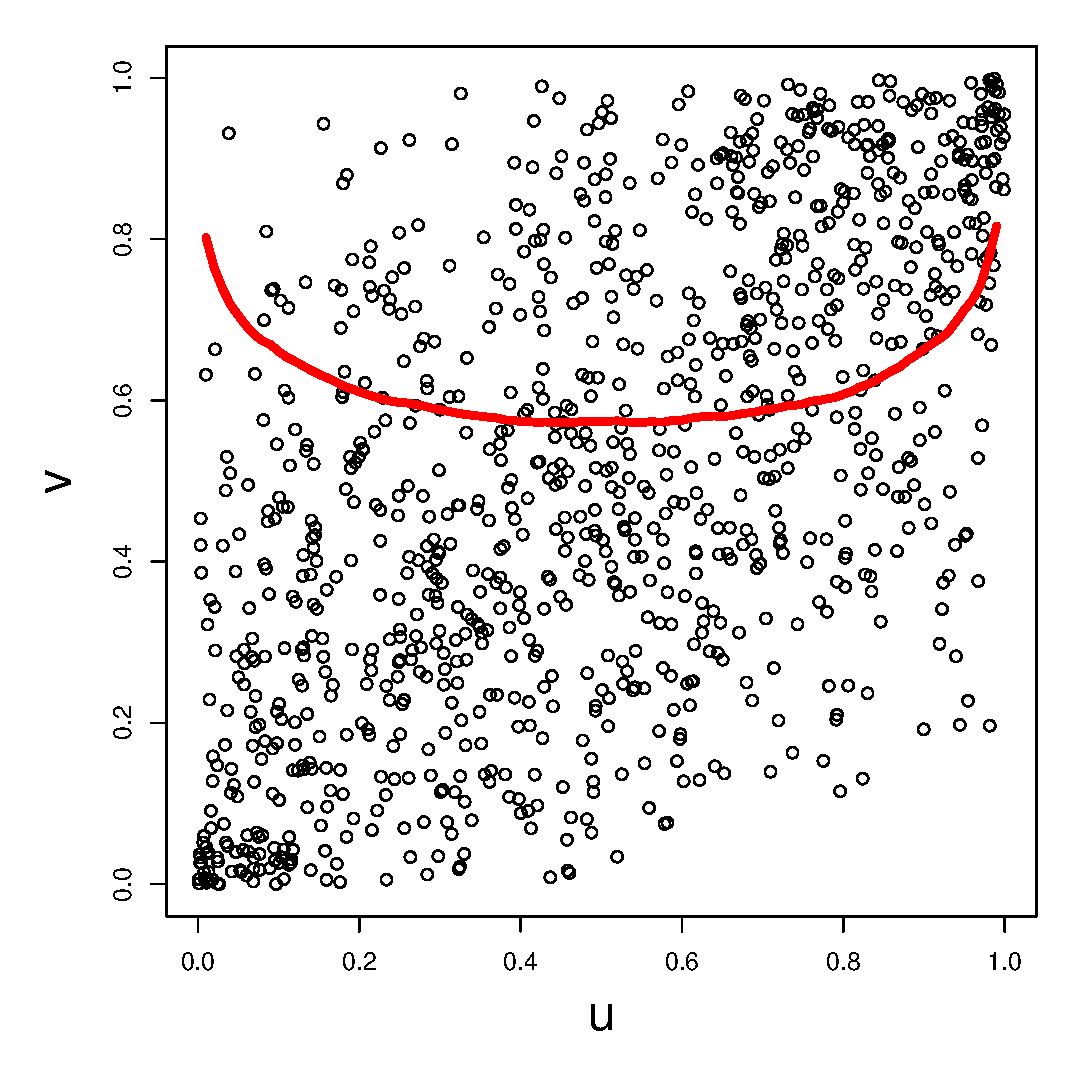
\includegraphics{normal.eps}}
            \resizebox{40mm}{!}{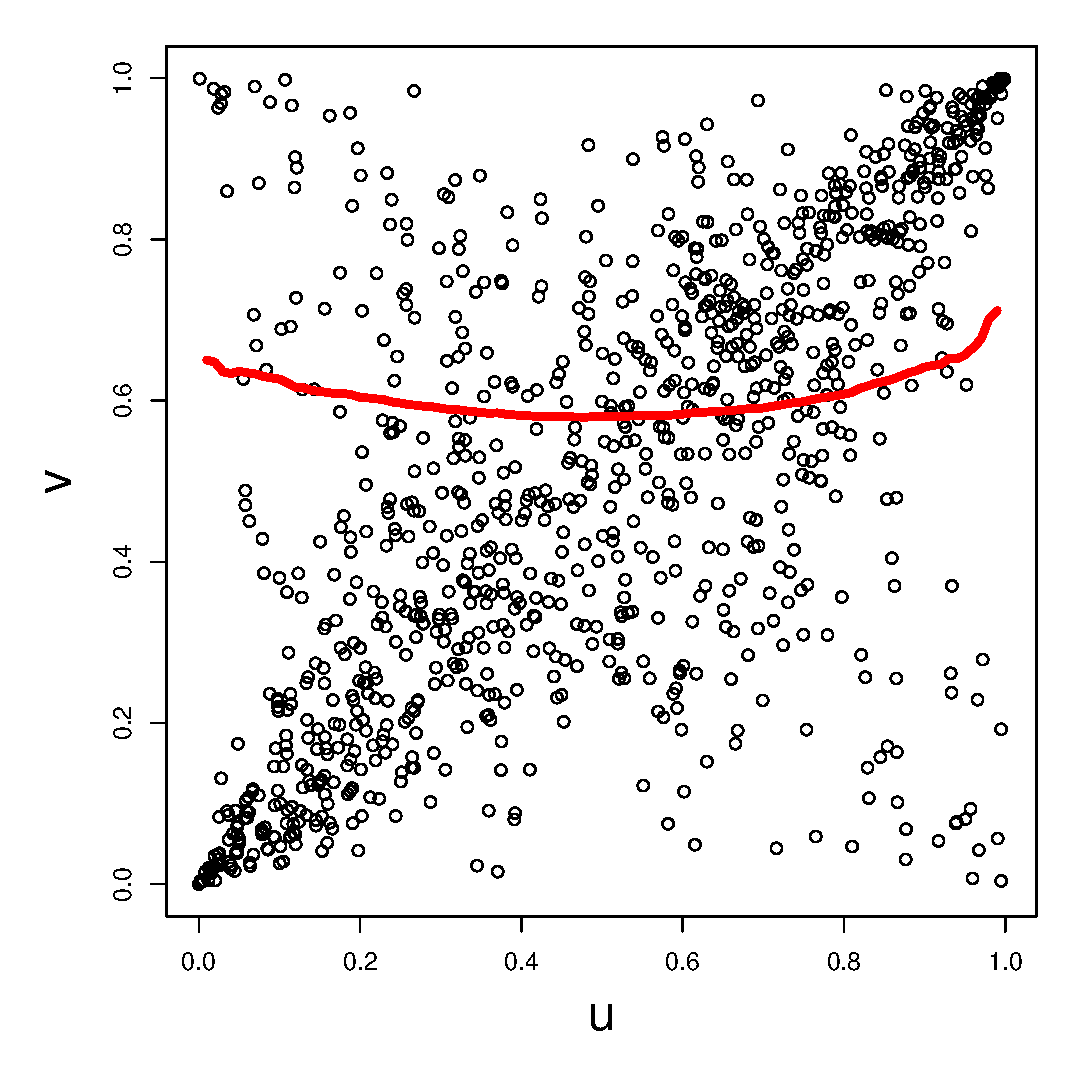
\includegraphics{student.eps}}
      \resizebox{40mm}{!}{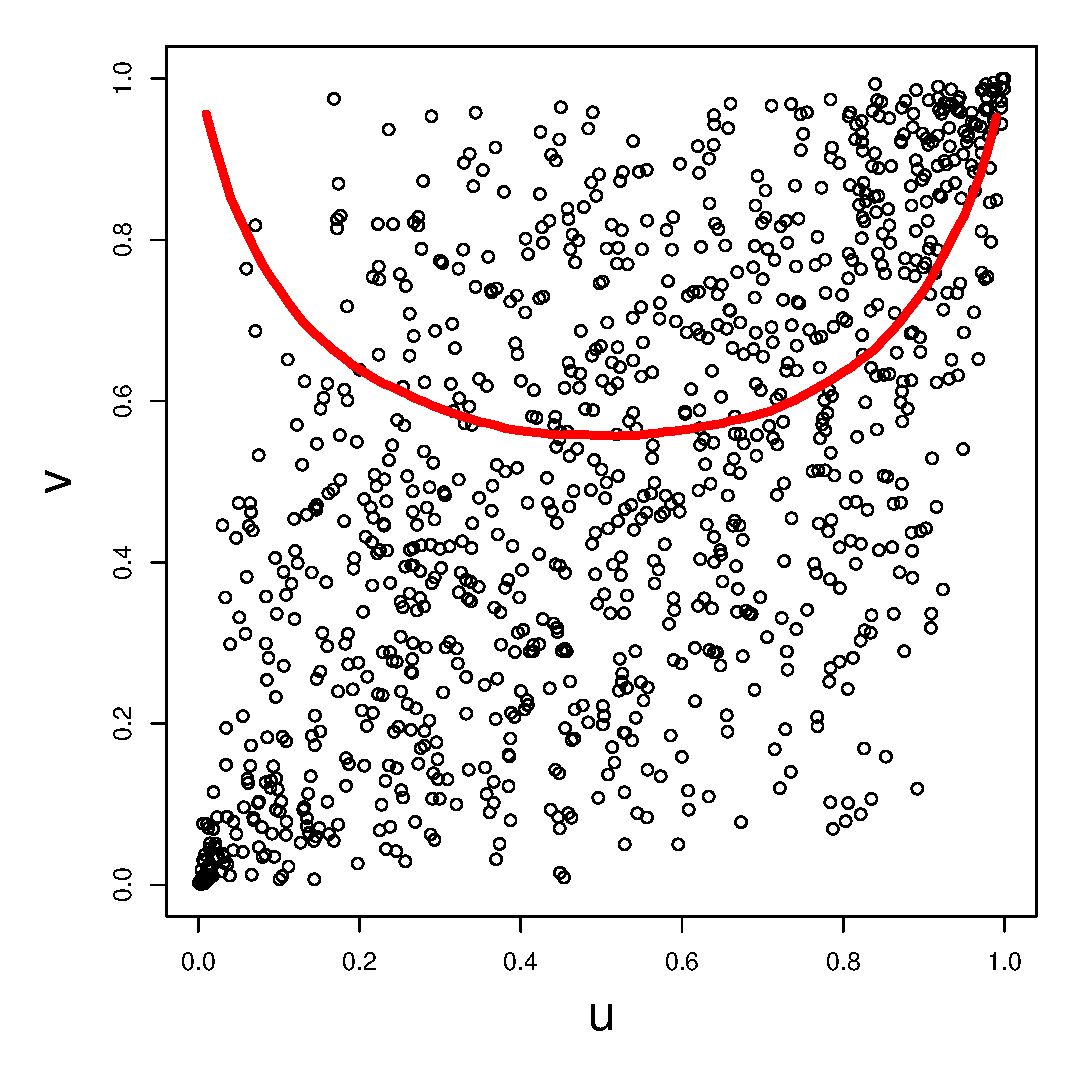
\includegraphics{structural2.eps}} \\
      \resizebox{40mm}{!}{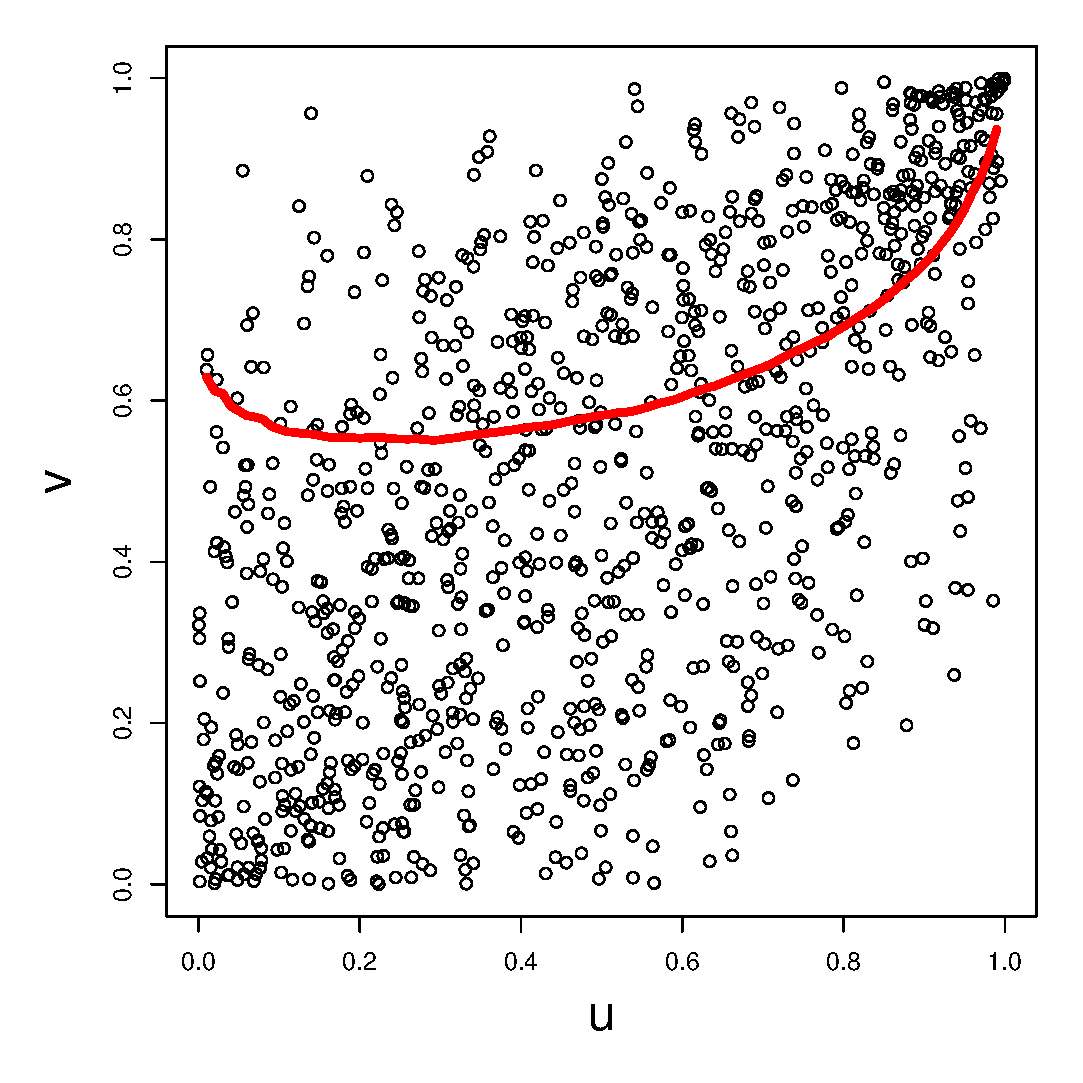
\includegraphics{gumbel.eps}}
            \resizebox{40mm}{!}{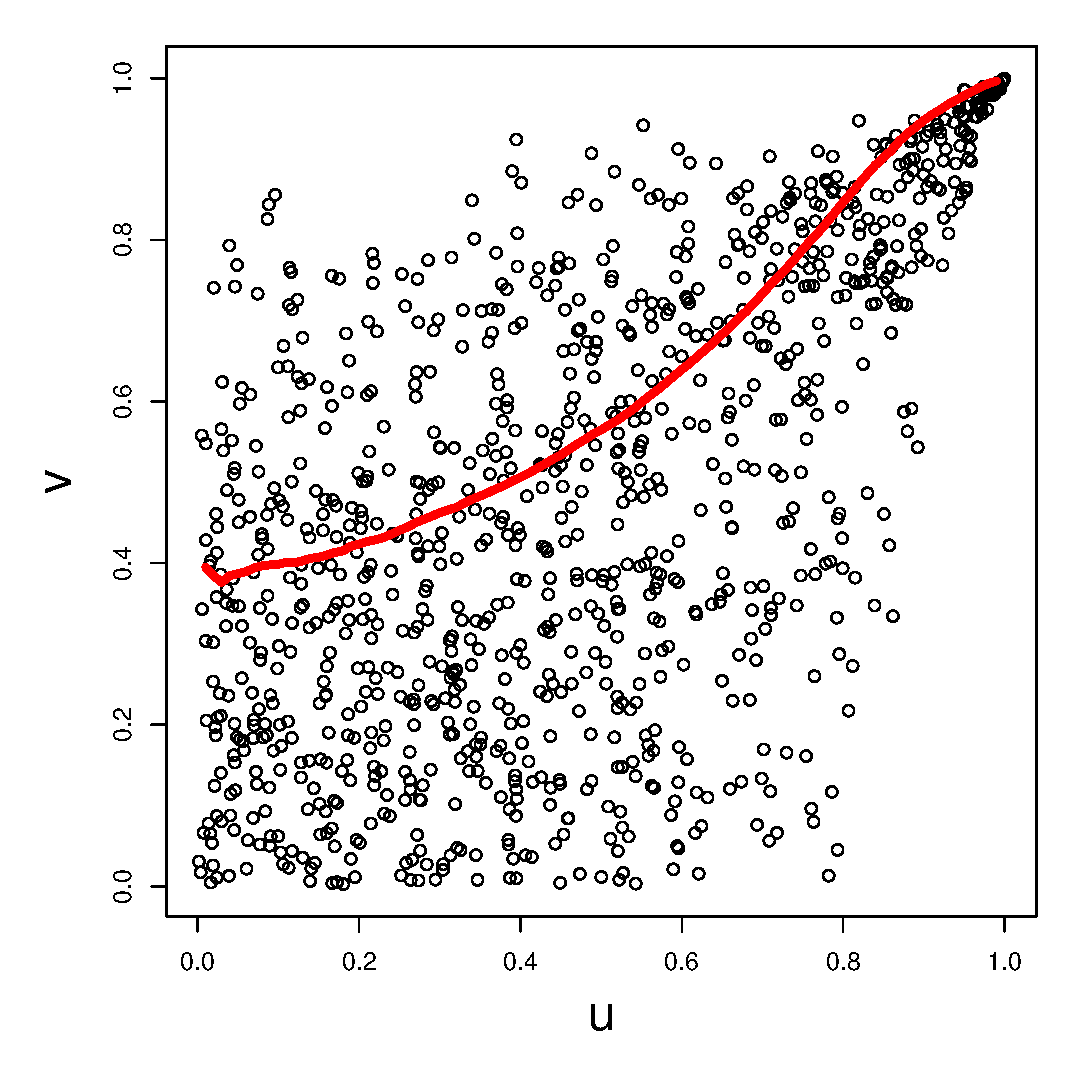
\includegraphics{structural1.eps}}
      \resizebox{40mm}{!}{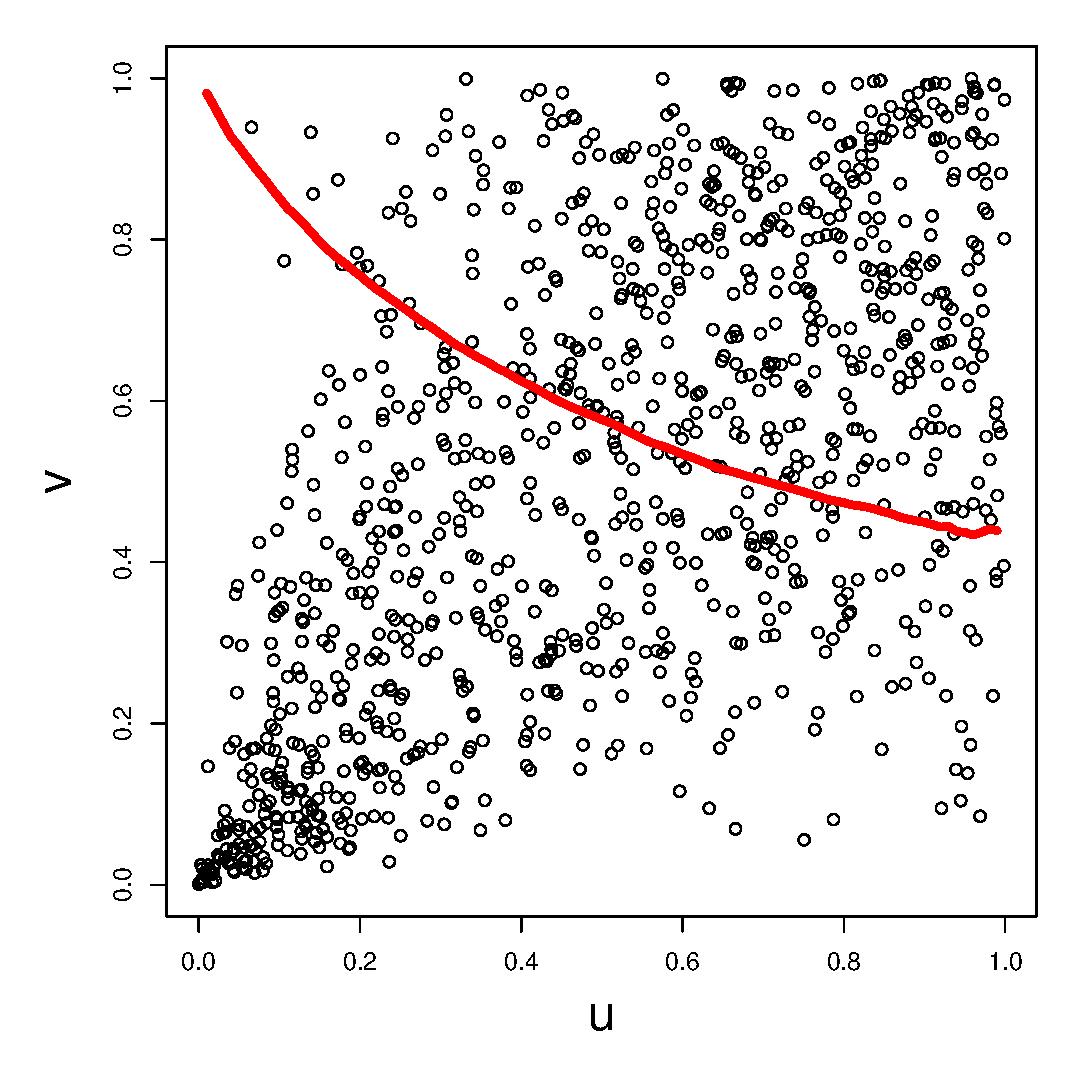
\includegraphics{clayton.eps}} \\
            \resizebox{40mm}{!}{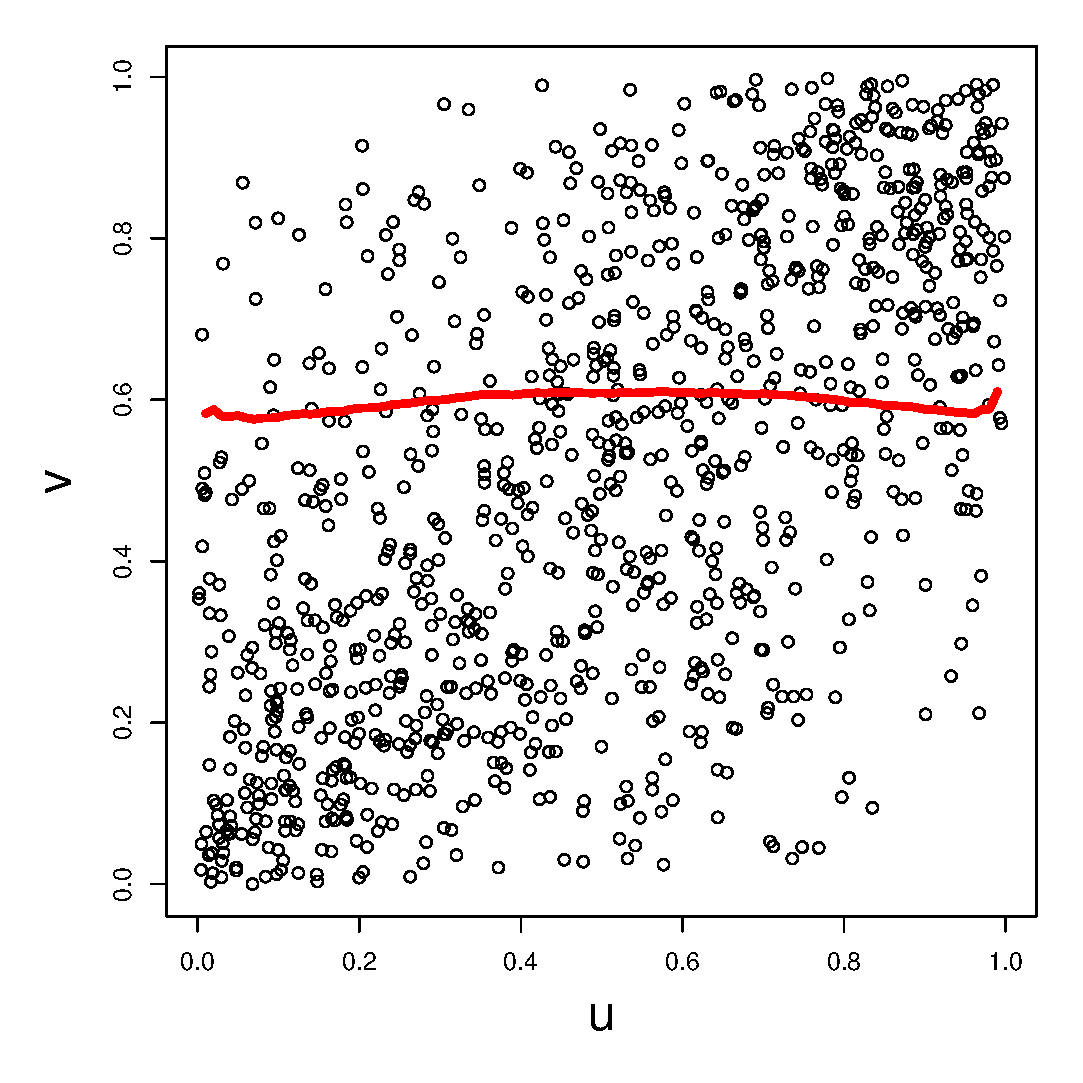
\includegraphics{frank.eps}}
            \resizebox{40mm}{!}{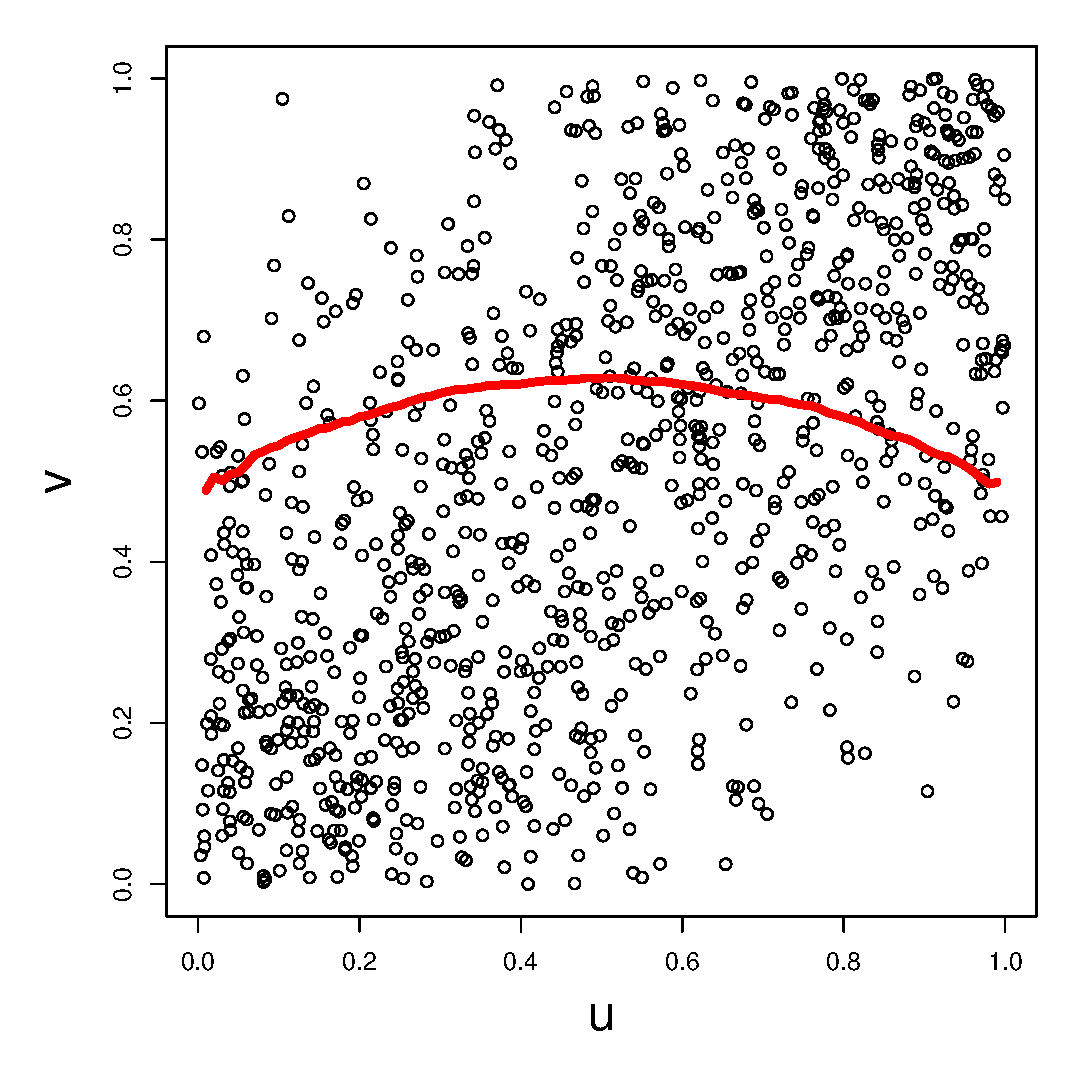
\includegraphics{structural3.eps}}
      \resizebox{40mm}{!}{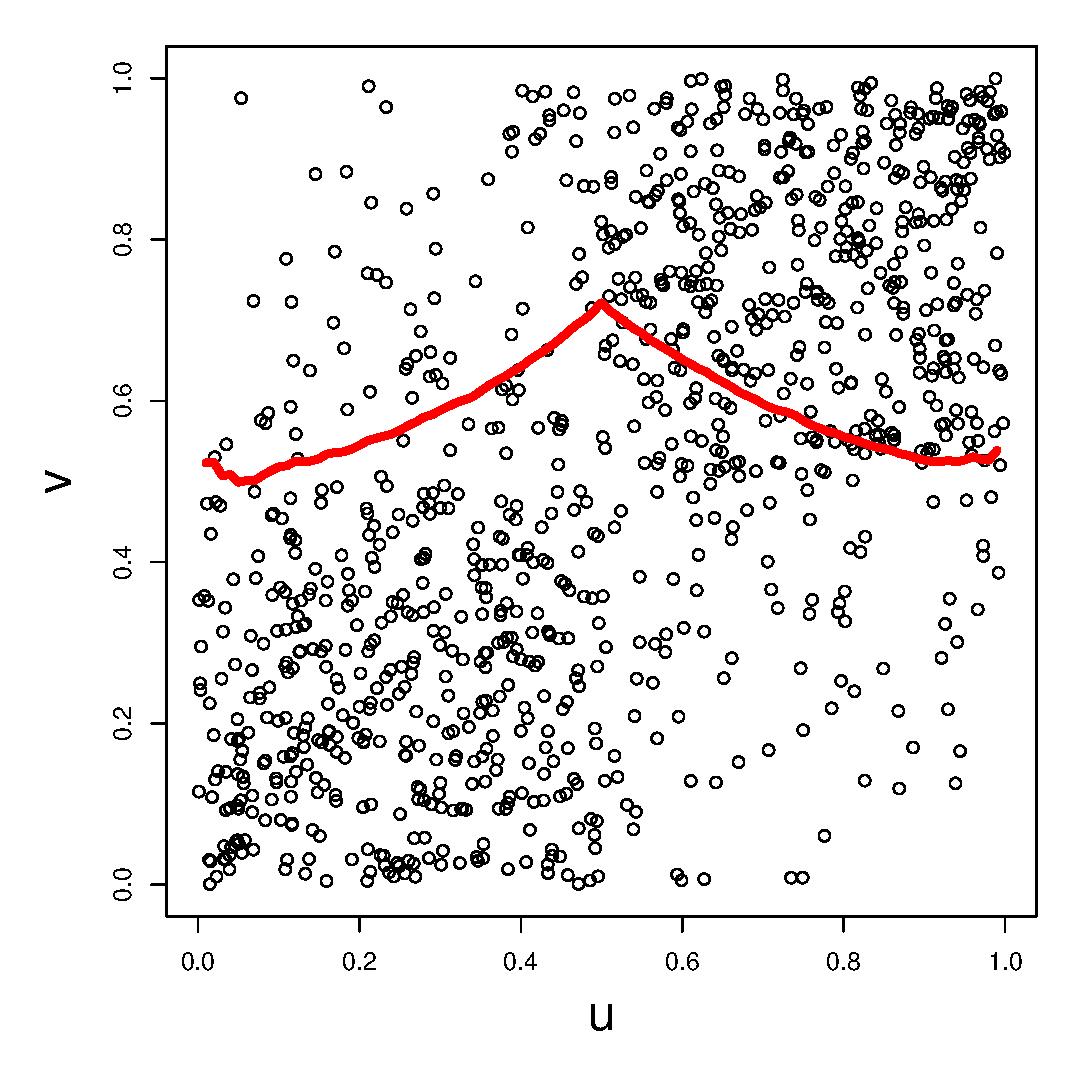
\includegraphics{structural4.eps}} \\
    \end{tabular}
    \caption{Copulas all  with the same  $\rho=0.6$ but different layer dependence curves $\ell_\alpha$ over $0\leq\alpha\le 1$ (red curves). The top 3 copulas display relatively strong tail dependence in both lower and upper tail.  The first two copulas in the middle three have relatively strong upper tail dependence and while the third has a high degree of lower tail dependence.   The bottom three copulas have relatively high local dependence in the middle of the distribution and less correlation in the tails.  Overall the panels illustrate how an overall given level of $\rho$ can mask a  range of local dependence: and that level dependence is an appropriate tool for assessing local dependence.}
    \label{fillustration}
  \end{center}
\end{figure}



\section{Layer dependence, discordance and dispersion}\label{sdecompose}

If a copula is symmetric in $u$ and $v$, then $\ell_\alpha$ is the same if $u$ and $v$ are exchanged.   Further, in this exchangeable case,
 layer dependence $\ell_\alpha$ is closely connected to measures the lack of discordance and dispersion.  In particular
\begin{equation}\label{decomposition}
\ell_\alpha = 1-2(1+\gamma_\alpha) \delta_\alpha \;,
\end{equation}
where
$$
\gamma_\alpha \equiv \cor\{(u\leq\alpha),(v>\alpha)\} =\cor\{(u>\alpha),(v\leq\alpha)\}\;,
$$
$$
\delta_\alpha \equiv\E\left\{(|u-v|)|(u-\alpha)(v-\alpha)<0\right\}  \; .
$$
A proof of \eref{decomposition} is  below.  The correlation $-1\leq\gamma_\alpha\leq 1$ measures the tendency for $(u,v)$ to be discordant at $\alpha$: opposite signs on $u-\alpha$ and $v-\alpha$.  The expectation $0\leq \delta_\alpha\leq 1$ measures the dispersion between discordant points $u$ and $v$ at $\alpha$.

The proof of \eref{decomposition} follows from
$$
\gamma_\alpha
=-\frac{\cov\{(u\leq\alpha),(v\leq\alpha)\}}{\var\{(u\leq\alpha)\}}
=\frac{\alpha^2-C(\alpha,\alpha)}{\alpha(1-\alpha)}   \;,
$$
and
$$
\delta_\alpha = 2 \E\left\{(u-v)(u>v)|(u-\alpha)(v-\alpha)<0\right\}
$$
$$
=  \frac{2\E\{(u-v)(u>v)(u>\alpha)(v\leq\alpha)\}}{2\E\{(u>\alpha)(v\leq\alpha)\}}
= \frac{\E\{(u-v)(u>\alpha)(v\leq\alpha)\}}{\alpha-C(\alpha,\alpha)}
$$
$$
= \frac{\E\{(u-v)(u>\alpha)\}-\E\{(u-v)(u>\alpha)(v>\alpha)\}}{\alpha-C(\alpha,\alpha)}
 = \frac{\E\{(u-v)(u>\alpha)\}}{\alpha-C(\alpha,\alpha)} \;.
$$
Substituting the above expressions for $\gamma_\alpha$ and $\delta_\alpha$ into the right hand side of \eref{decomposition} yields the expression for $\ell_\alpha$ in \eref{gapexp}, completing the proof.

Result \eref{decomposition} explains the behaviour of layer dependence curves in \fref{fillustration}. Layer dependence $\ell_\alpha$ is larger if there are fewer discordant pairs at $\alpha$, and discordant pairs at $\alpha$ are closer to the $45^\circ$ degree line. The former indicates smaller $\gamma_\alpha$ and the latter indicates smaller $\delta_\alpha$. Opposite observations apply for small $\ell_\alpha$. If $\ell_\alpha=1$ then $\gamma_\alpha=-1$ or $\delta_\alpha=0$, implying $u$ and $v$ are simultaneously below or above $\alpha$ and $u=v$ for discordant pairs. If $\ell_\alpha=1$  in an interval, then $u=v$  in the same interval.

\fref{finterpretation} illustrates the relationship between layer dependence, discordance and dispersion in \eref{decomposition} using two copulas with $\ell_\alpha=1$ and $\ell_\alpha=0.86$ at $\alpha=0.75$. When $\ell_\alpha=1$, there is no discordance or dispersion at $\alpha$. As $\ell_\alpha$ decreases from $1$, the number of discordant pairs and their dispersion increases.

\begin{figure}
  \begin{center}
    \begin{tabular}{cc}
      \resizebox{60mm}{!}{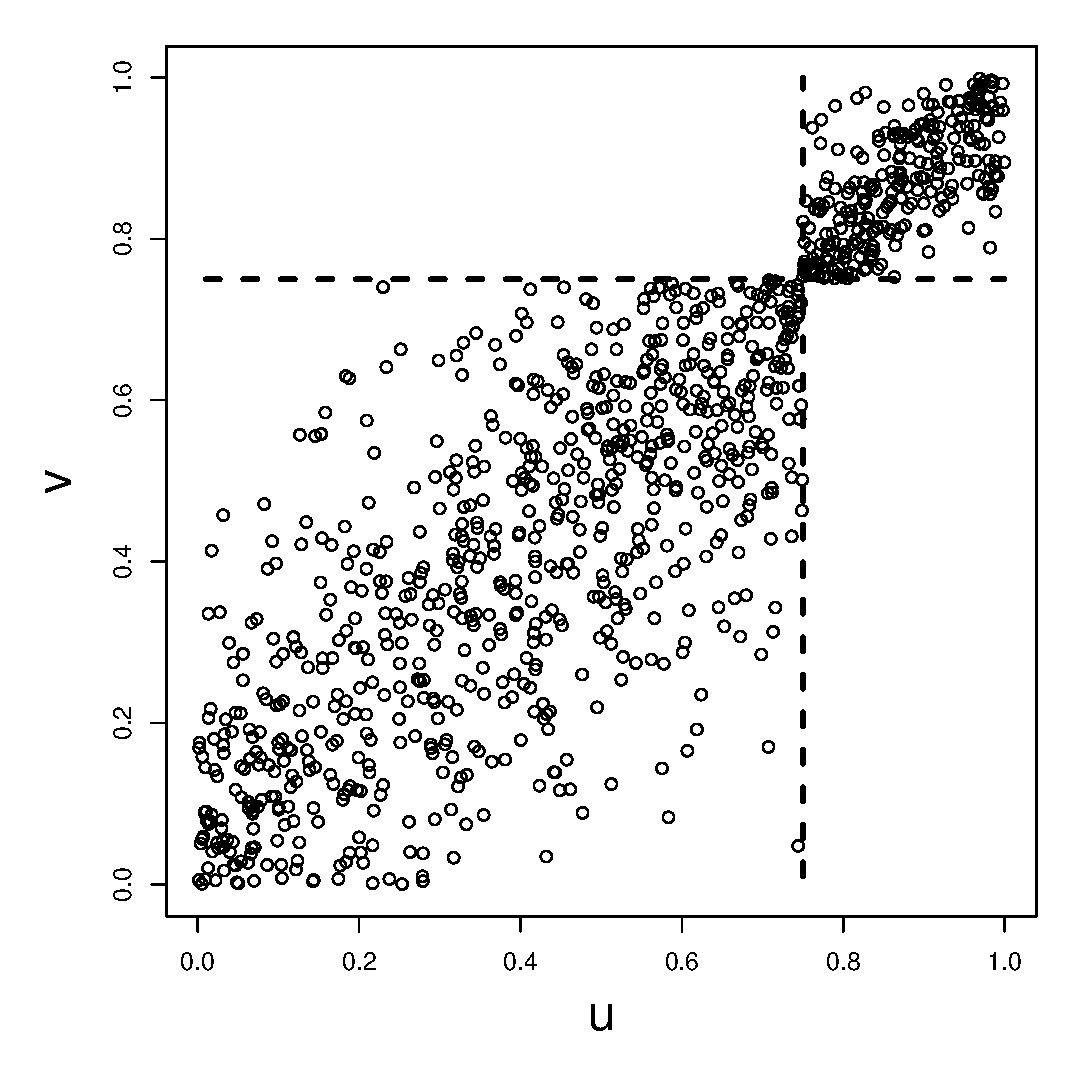
\includegraphics{perfect.eps}}
      \resizebox{60mm}{!}{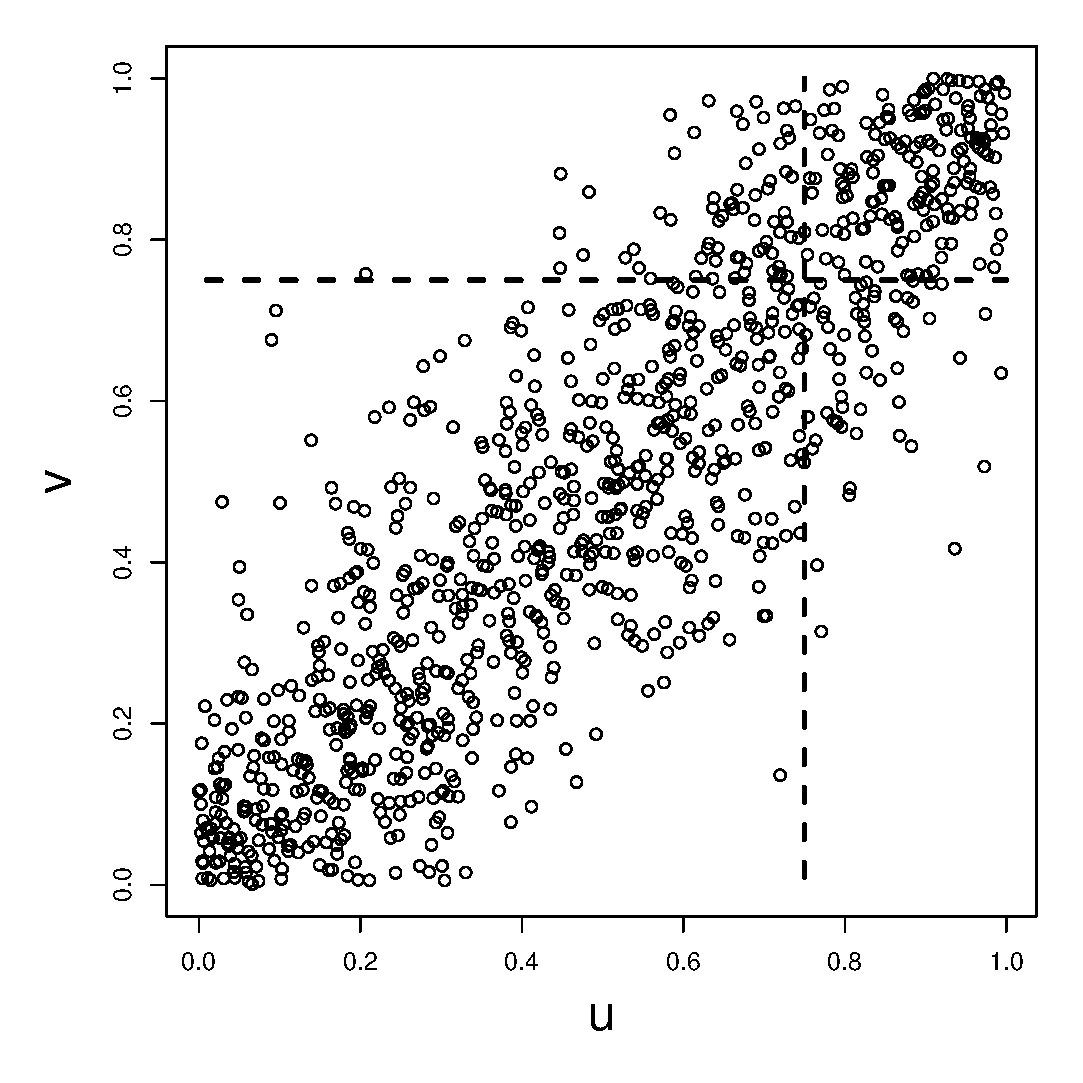
\includegraphics{imperf.eps}} \\
    \end{tabular}
    \caption{The left and right panel  show $\ell_{0.75}=1$ and $\ell_{0.75}=0.86$, respectively. In the left panel, $\gamma_{0.75}=-1$ and $\delta_{0.75}=0$. In the right panel, $\gamma_{0.75}=-0.65$ and $\delta_{0.75}=0.21$.  }
    \label{finterpretation}
  \end{center}
\end{figure}







\begin{comment}

The probability of discordance is
$$
\E[\{(u-\alpha)(v-\alpha)<0\}]
=2\alpha\{(1-\alpha)(\gamma_\alpha+\alpha^2)-1\} \;.
$$


The following illustrates \eref{decomposition} using the income-education example introduced in \sref{sintroduction}. Given $\alpha$, classify individuals as ``concordant" or ``discordant." The former are those with income and education both below or above $\alpha$. The latter are remaining individuals. Scale the proportion of concordant individuals to yield $\gamma_\alpha^*$. Calculate average dispersion $\delta_\alpha$ as twice the average difference between income and education of discordant individuals. Combine $\gamma^*_\alpha$ and $\delta_\alpha$ using \eref{decomposition} to yield $\alpha$-layer dependence $\ell_\alpha$. Layer dependence decreases with the proportion of discordant individuals and their average income-education dispersion.




\fref{fdecomposition} illustrates the decomposition of percentile rank gap by separately showing the standardised concordance probability $\gamma_\alpha^*$ and dispersion $\delta_\alpha$. The same four copulas as in \fref{fillustration} are applied.

\begin{figure}
  \begin{center}
    \begin{tabular}{cc}
      \resizebox{60mm}{!}{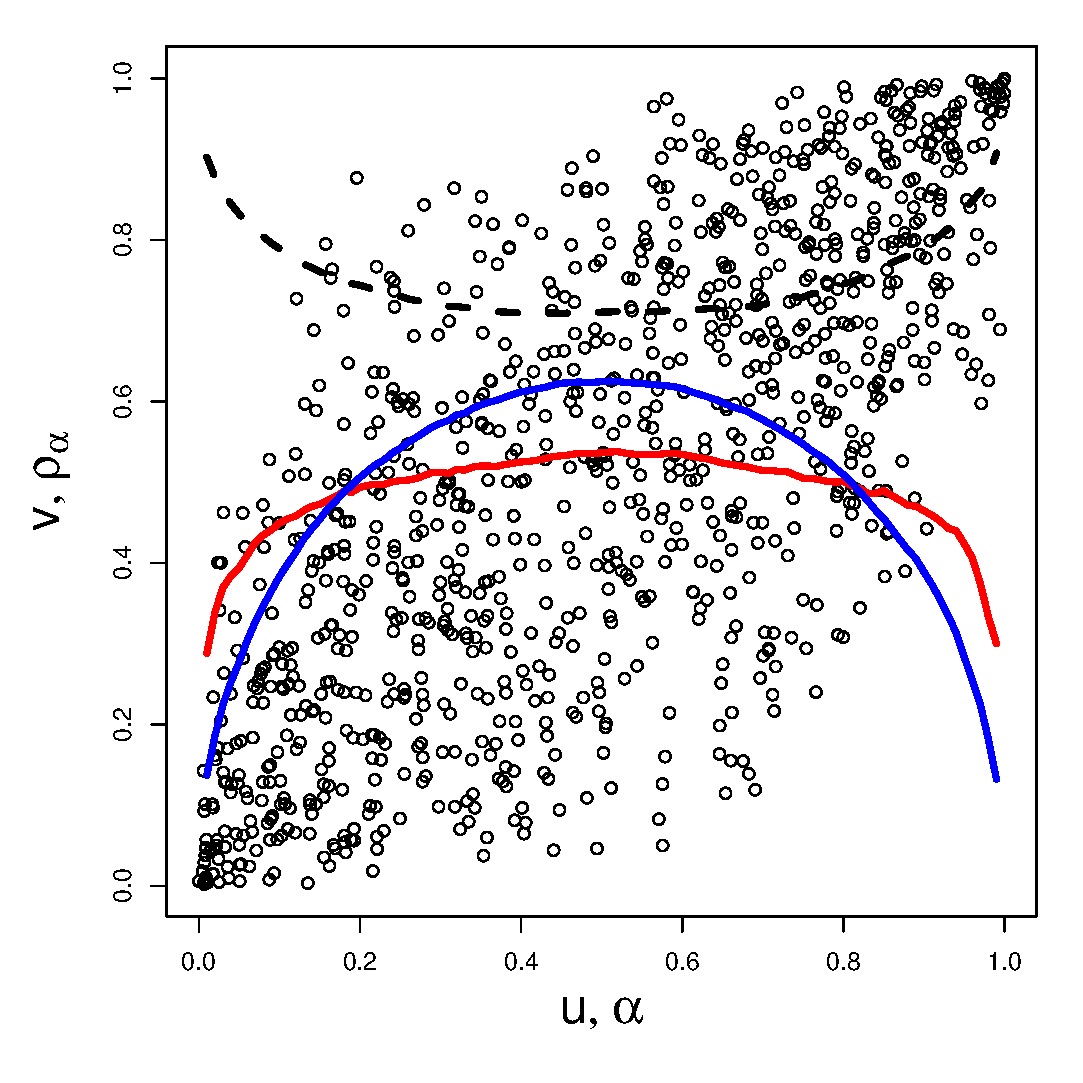
\includegraphics{normaldecom.eps}}
      \resizebox{60mm}{!}{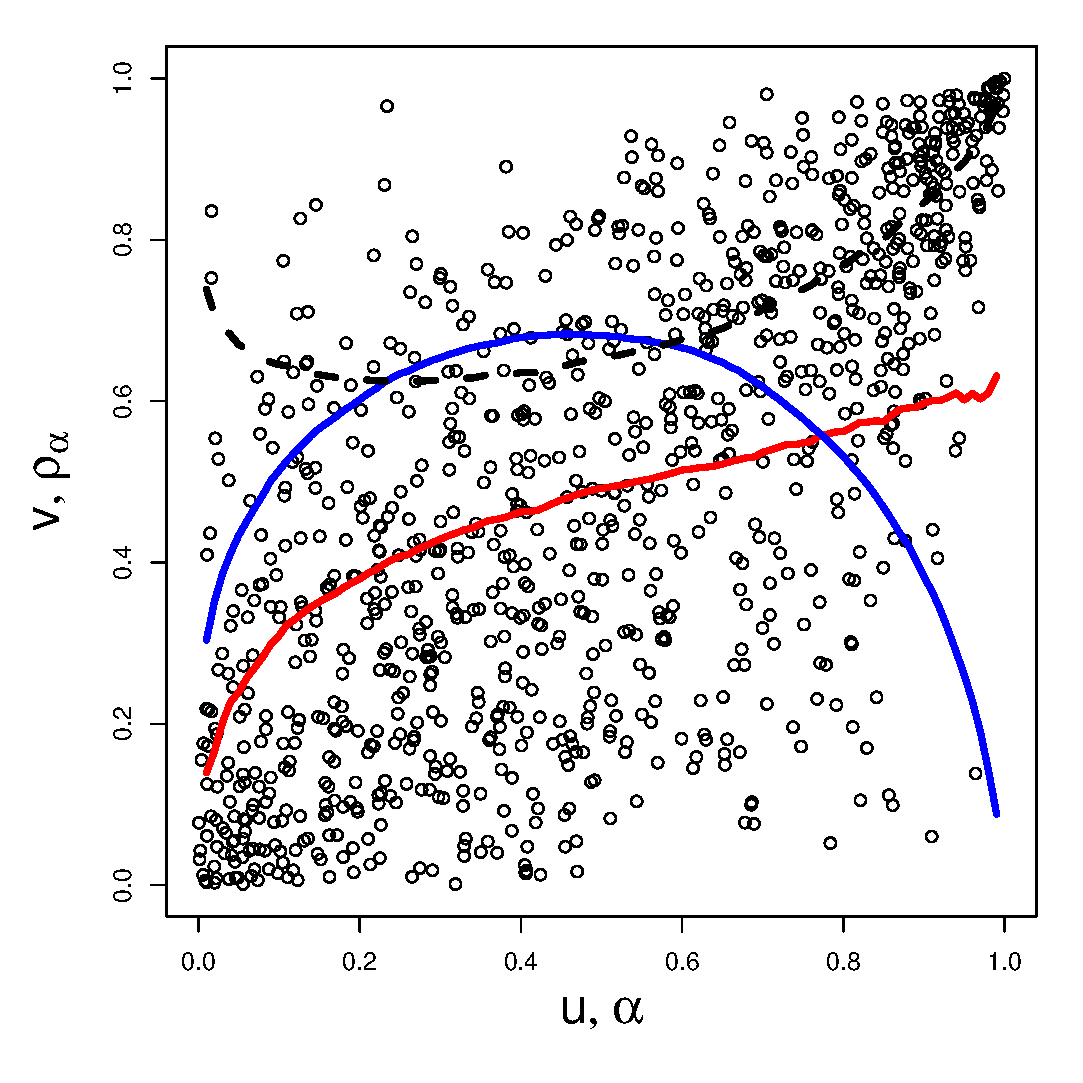
\includegraphics{gumbeldecom.eps}} \\
      \resizebox{60mm}{!}{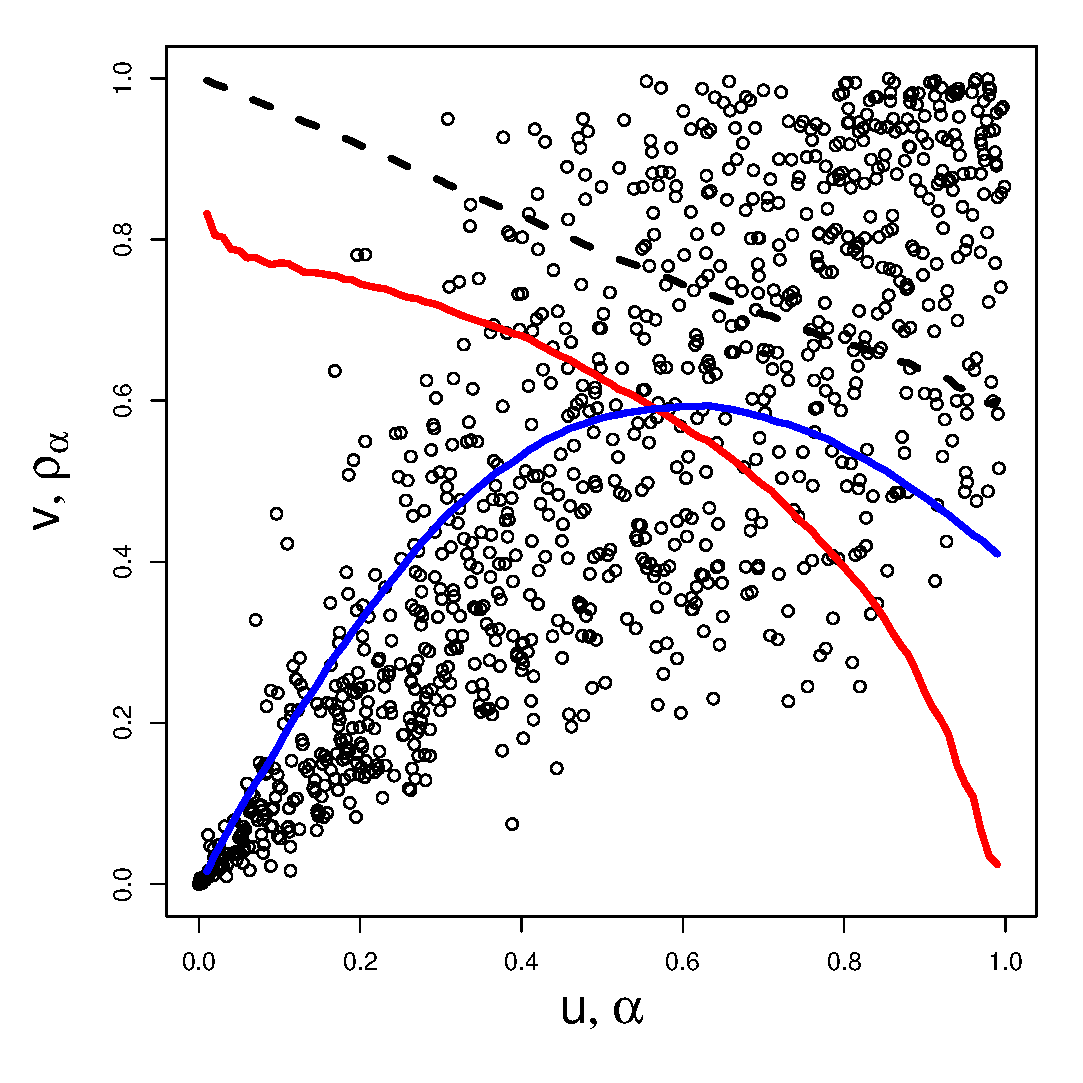
\includegraphics{claytondecom.eps}}
      \resizebox{60mm}{!}{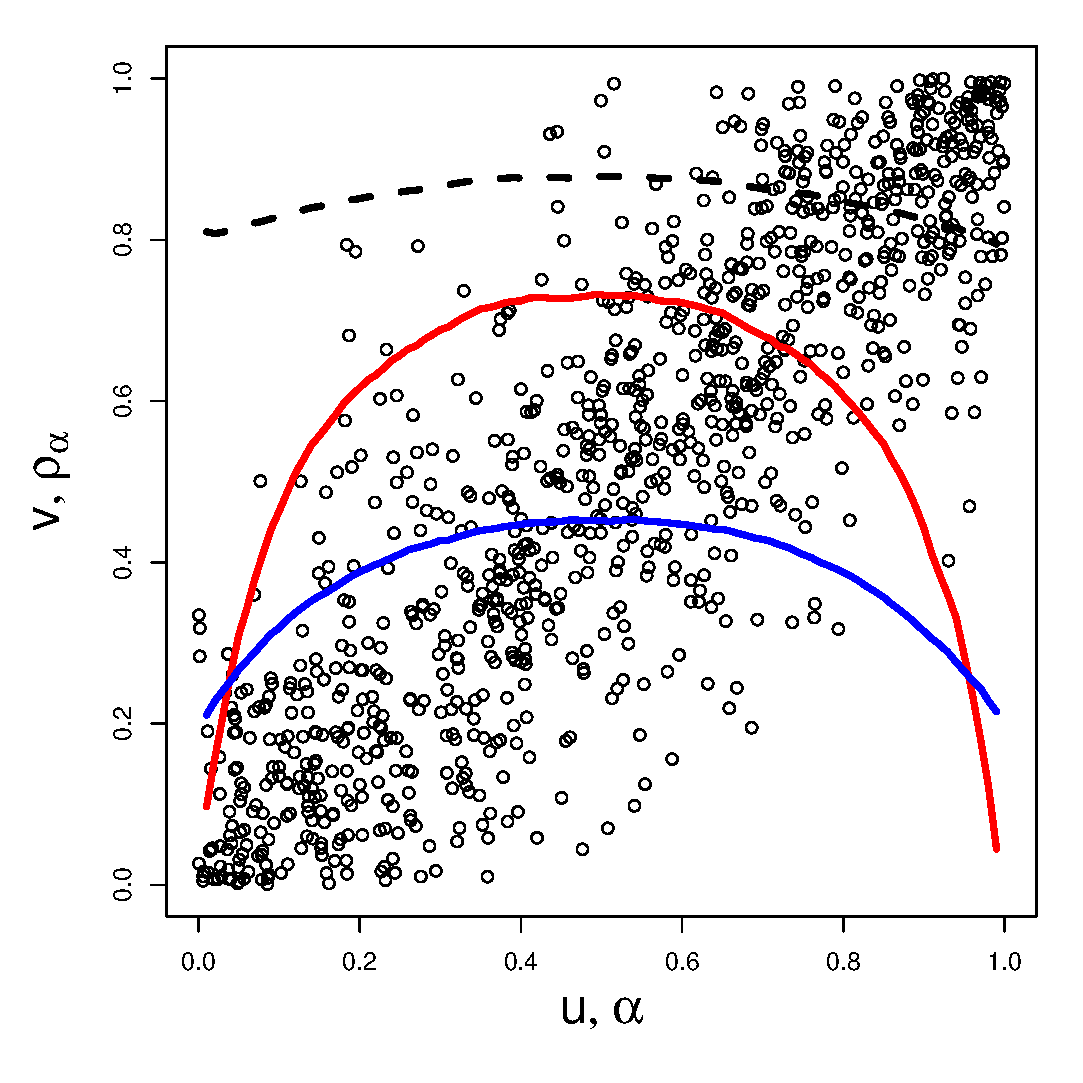
\includegraphics{frankdecom.eps}} \\
    \end{tabular}
    \caption{Standardised concordance probability $\sgamma^*_\alpha$ (red line) and dispersion $\delta_\alpha$ (blue line) for a Gaussian copula (top left), Gumbel copula (top right), Clayton copula (bottom left) and Frank copula (bottom right). Percentile rank gap (dotted black line) is also shown.}
    \label{fdecomposition}
  \end{center}
\end{figure}



Manipulating the expression for $\ell_\alpha$ in \eref{relationship} yields
$$
\ell_\alpha = 1- \frac{\E\{d(u,v) z_\alpha\}}{\alpha(1-\alpha)}  \cq \ell = 1-6\int_0^1 \E\{d(u,v)z_\alpha\} \de \alpha \;.
$$
where the above result for $\ell$ applies $\ell=\int_0^1 w_\alpha \ell_\alpha \de \alpha$, $w_\alpha\equiv 6\alpha(1-\alpha)$. Hence $\rho_S$ is negatively related to the average dispersion between discordant $(u,v)$ over all $\alpha$.






========== Haven't done much below here =============

\subsection{Income-education interpretation}

The following interprets layer dependence using an income-education example. Consider education $(u)$ and income $(v)$ rankings of individuals in a population, with $0$ and $1$ representing lowest and highest, respectively. Given $\alpha$, divide the population into two segments based on education: $u\leq \alpha$ and $u>\alpha$. Measure average income in each segment. From \eref{gapexp}, $\alpha$-layer dependence is twice the gap in average income between the two segments.

Suppose $\ell_\alpha$ is close to one for $\alpha=0.95$. This implies highly educated individuals (top $5\%$) are likely to be high income earners (top $5\%$), and vice versa. Few individuals have top $5\%$ education and income not in top $5\%$ or vice versa, and their average education-income difference is small. Hence there is strong income-education dependence at the $95$th percentile education layer. Dependence is perfect if $\ell_\alpha=1$. If $\ell_\alpha=0$ then average income is equal between individuals with education below and above top $5\%$, implying independence at the $95$th percentile education layer. The same argument applies to $\ell_\alpha$ for other values of $\alpha$.

This paper formulates layer dependence in terms of $u$ and $v$, in this case income and education ranks. Section \sref{soriginal} discusses an analogous definition of layer dependence between observed random variables $x$ and $y$, or original measurements of income and education.

\end{comment}





\section{Coherence properties of layer dependence}\label{scoherence}


Layer dependence $\ell_\alpha$ satisfies five ``coherence" properties. These properties are  extensions of  properties applying to Spearman's $\rho$.
\begin{itemize}

\item \textbf{Bounds}: Layer dependence lies between $-1$ and $1$: $-1 \le\ell_\alpha \le 1$ for all $\alpha$.
Hence layer dependence is bounded in the same way as  $\rho_S$.

\item \textbf{Perfect dependence}: Constant layer dependence of $-1$ or $1$ are equivalent to countermonotonicity and comonotonicity.
Thus $\ell_\alpha=-1$ for all $\alpha$ if and only if  $v=1-u$ while $\ell_\alpha=1$ for all $\alpha$ if and only if  $v=u$.

\item \textbf{Independence}: If $u$ and $v$ are independent then $\ell_\alpha\equiv 0$.   The converse is not true -- zero layer dependence does not imply independence as shown by the following counterexample. Assume $v=u$ and $v=1-u$ with equal probability. Then $\E(v|u=t)=0.5$ for all $0\leq t\leq 1$ implying $\E(v|u>\alpha)=\E(v|u\leq\alpha)=0.5$. Hence $\ell_\alpha=0$ from \eref{gapexp}. However $u$ and $v$ are not independent.

\item \textbf{Symmetry}: Ranking $v$ in the opposite direction switches the sign of layer dependence. Doing the same to $u$ (the random variable decomposed into layers) switches the sign of layer dependence and flips the layer dependence curve $\ell_\alpha$ about $\alpha=0.5$. Changing the ranking order of both $u$ and $v$ only flips the layer dependence curve.

\item \textbf{Ordering}: Higher correlation order \citep{dhaene2009correlation} leads to higher layer dependence. Consider bivariate uniform $(u^*,v^*)$ exceeding $(u,v)$ in correlation order: $C^*(a,b)\geq C(a,b)$ for all $0\leq a,b\leq 1$, where $C^*$ is the joint distribution of $(u^*,v^*)$. Then
$
\ell^*_\alpha \geq \ell_\alpha$,   $0\leq\alpha\leq 1$
where $\ell_\alpha^*$ denotes the $\alpha$--layer dependence of $(u^*,v^*)$. Hence greater dependence leads to higher layer dependence across all percentiles.

\end{itemize}
Independence, symmetry and ordering properties follow from the definition of layer dependence in \eref{definition}. From \eref{gapexp}, constant layer dependence of one implies $\E(v|u>\alpha)=(\alpha+1)/2$ and $\E(v|u=\alpha)=\alpha$, for all $0\leq\alpha\leq 1$, hence $v=u$. Similarly constant layer dependence of minus one implies $v=1-u$. The ordering property holds since higher correlation order implies larger covariances \citep{dhaene2009correlation}. Prove the bounds property by combining ordering and perfect dependence properties, and noting countermonotonicity and comonotonicity represent minimum and maximum correlation order, respectively. Detailed proofs of the coherence properties of layer dependence are discussed in the appendix in section \aref{app1}.


Most of the above layer dependence properties can be expressed using copulas. For the independence property, $C(u,v)=uv$ implies $\ell_\alpha=0$ and for the perfect dependence property, $C(u,v)=\min(u,v)$ is equivalent to $\ell_\alpha=1$ and $C(u,v)=\max(u+v-1,0)$ is equivalent to $\ell_\alpha=-1$. For the symmetry property, the copula of $(u,1-v)$ is $u-C(u,1-v)$ and has layer dependence $-\ell_\alpha$. Similarly the copula of $(v,1-u)$ is $v-C(1-u,v)$ and has layer dependence $-\ell_{1-\alpha}$. Lastly the copula of $(1-u,1-v)$ is the survival copula $u+v-1+C(1-u,1-v)$ of $C$ and has layer dependence $\ell_{1-\alpha}$.



\begin{comment}


\subsection{Copula comparison using percentile gap}

The following compares copulas based on their percentile gap values. The comparison yields a goodness-of-fit test when modeling past data using copulas. \fref{comparison} plots upper conditional tail expectations $\E(v|u>\alpha)=0.5(\alpha\ell_\alpha+1)$ of the copulas in \fref{fillustration} against the Gaussian copula. Given $\alpha$, points above the $45^{o}$ line indicates the copula has percentile gap exceeding that of the Gaussian copula. Vice versa for points below the $45^{o}$ line.


 we can easily simulate $\tau_\alpha$ paths as $(1/2)+\e^{(1-\alpha)}+\eps_\alpha$.

\begin{figure}
  \begin{center}
    \begin{tabular}{ccc}
      \resizebox{40mm}{!}{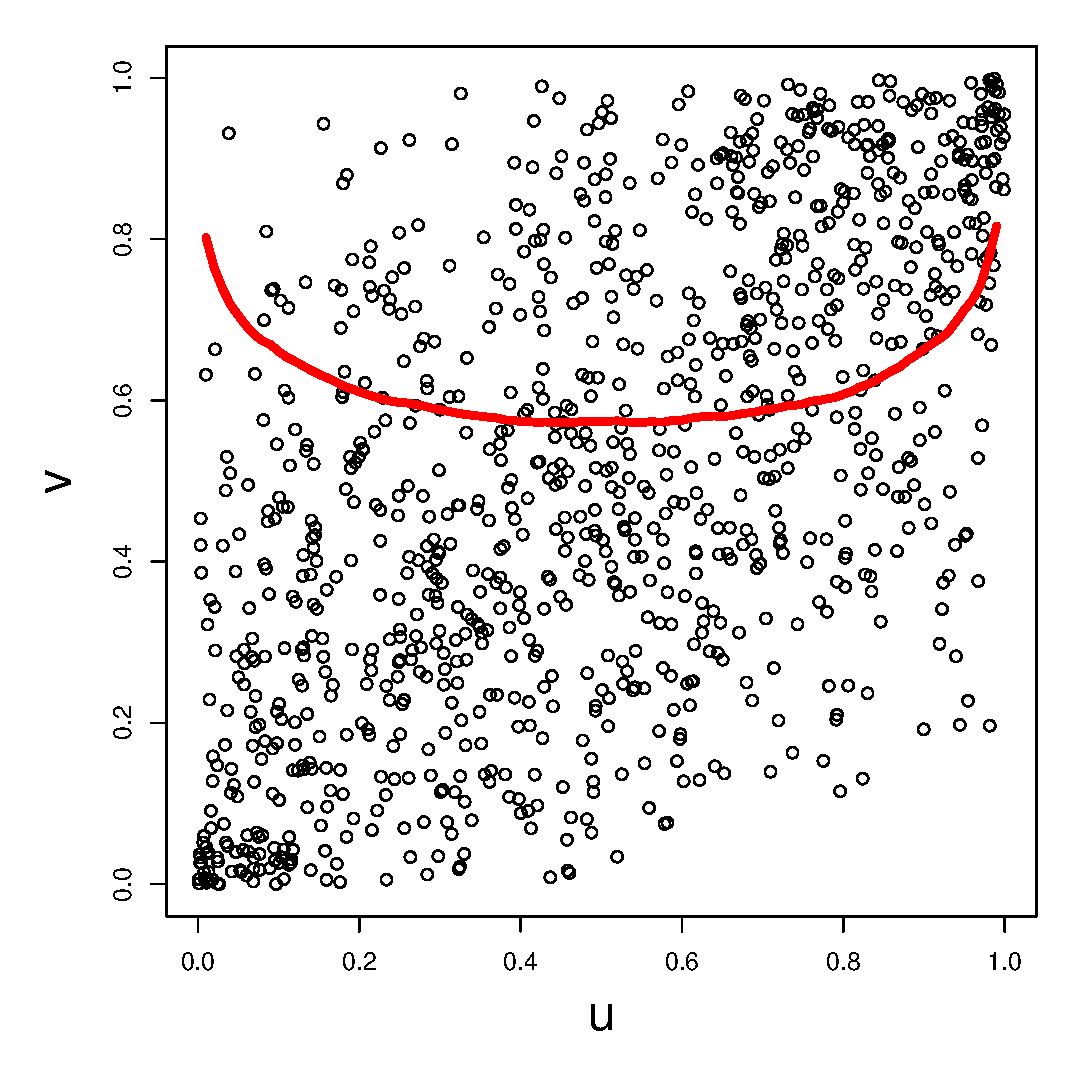
\includegraphics{normal.eps}}
            \resizebox{40mm}{!}{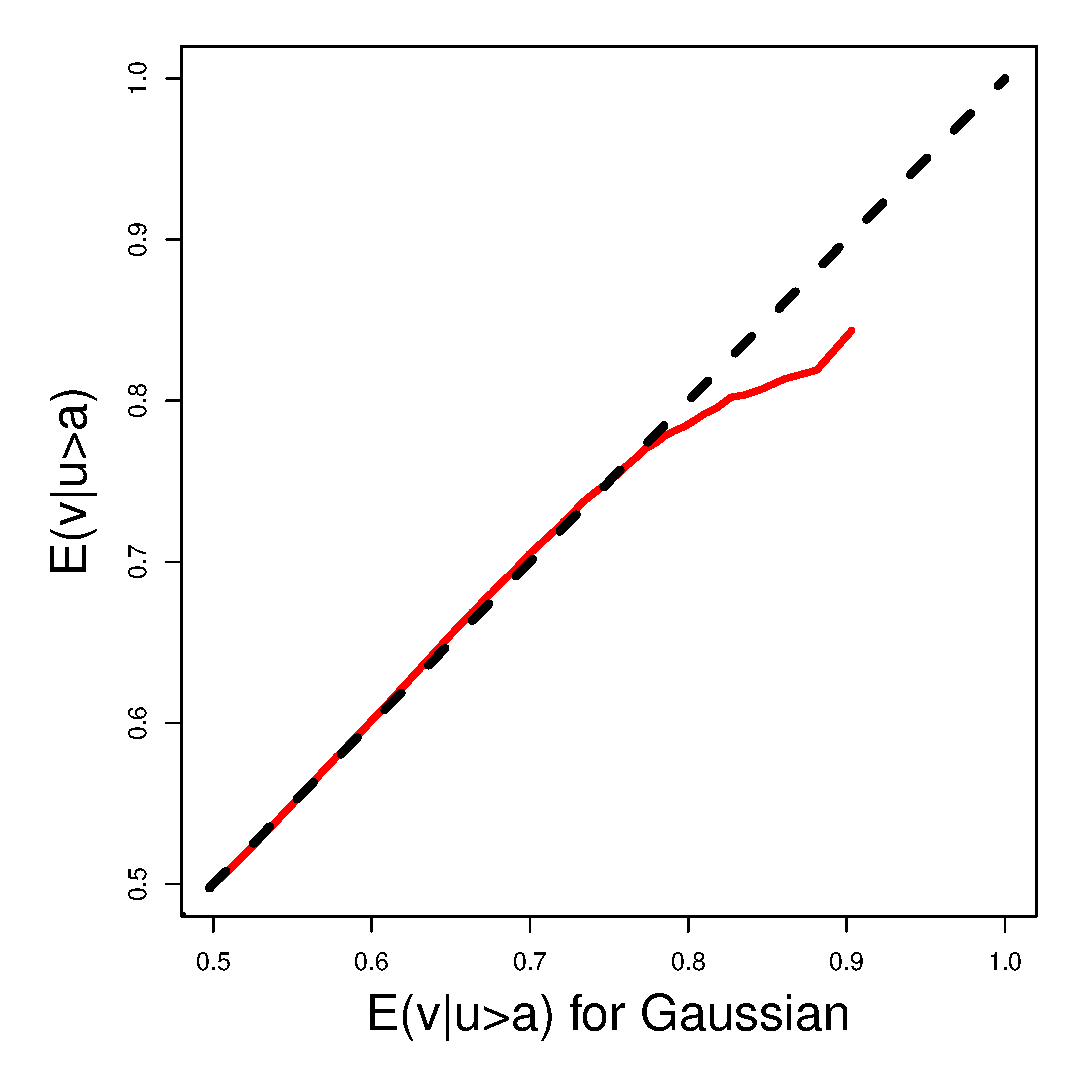
\includegraphics{studentvs.eps}}
      \resizebox{40mm}{!}{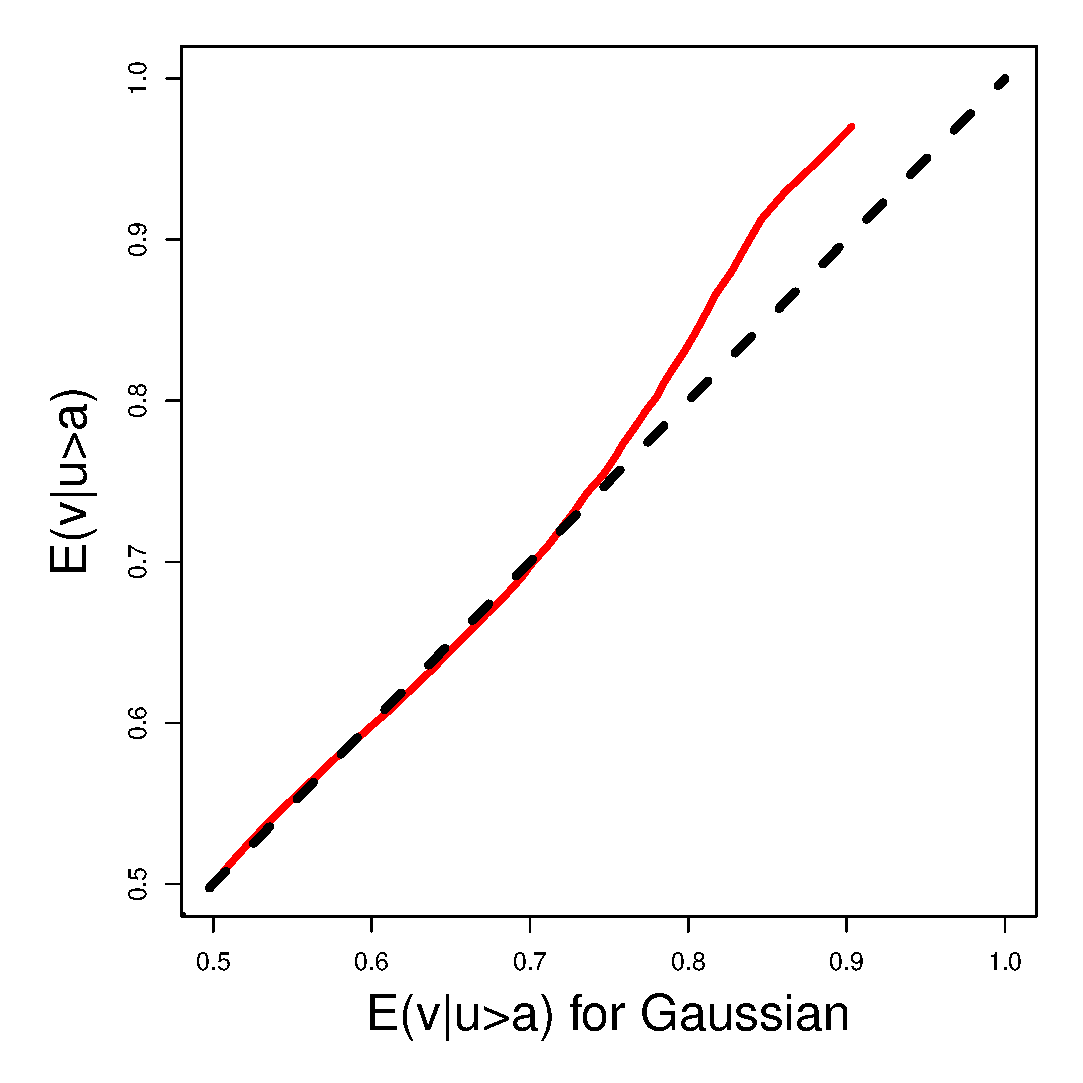
\includegraphics{structural2vs.eps}} \\
      \resizebox{40mm}{!}{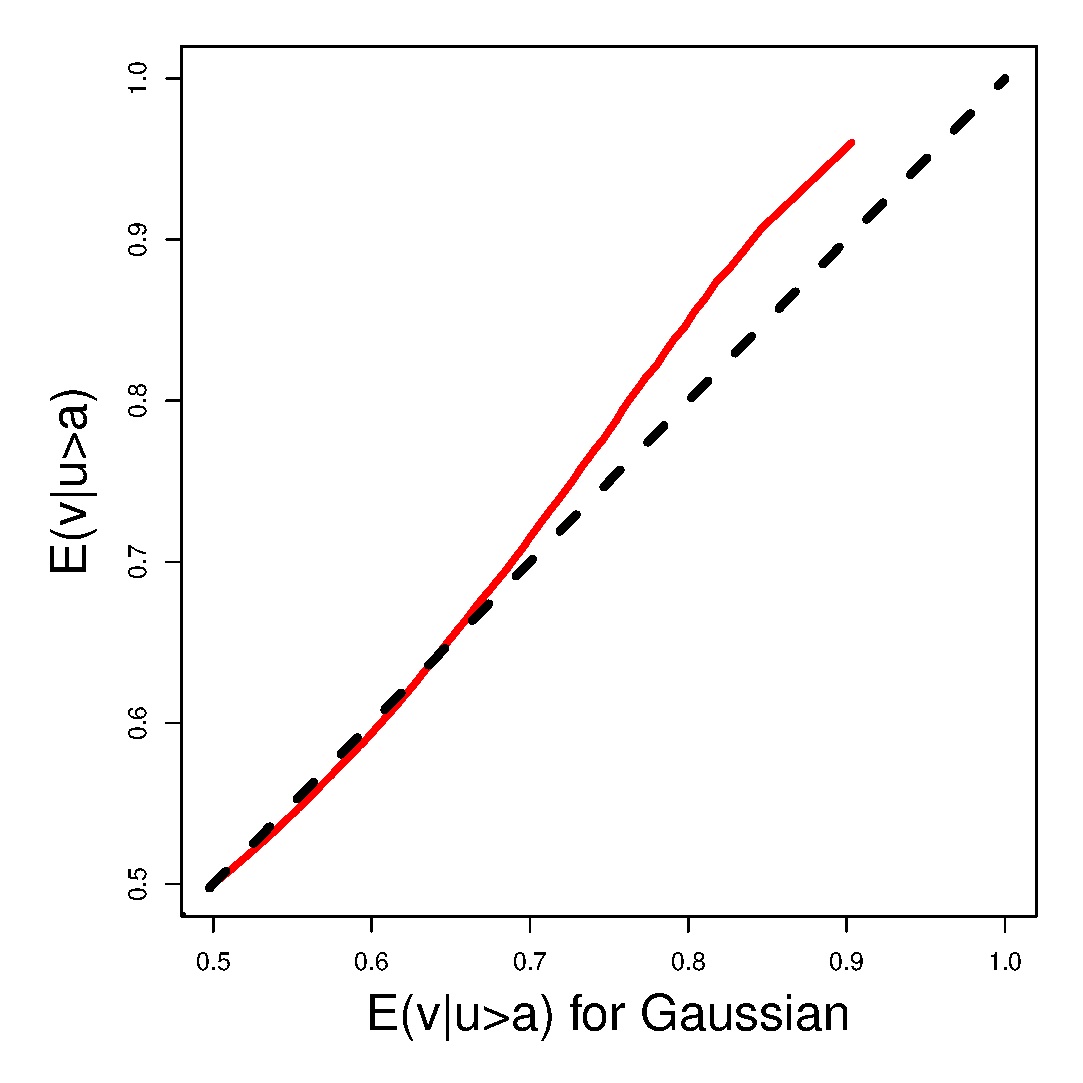
\includegraphics{gumbelvs.eps}}
            \resizebox{40mm}{!}{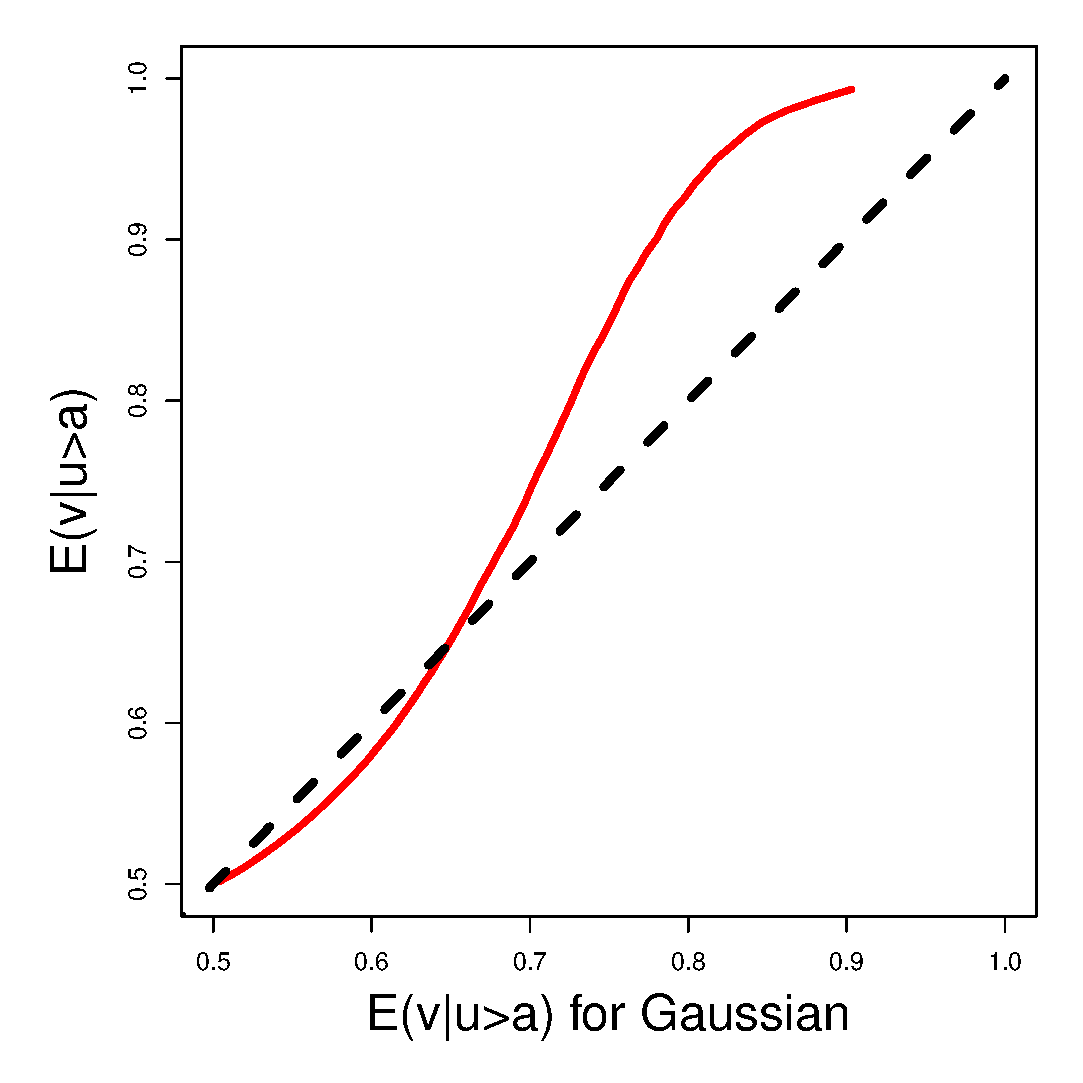
\includegraphics{structural1vs.eps}}
      \resizebox{40mm}{!}{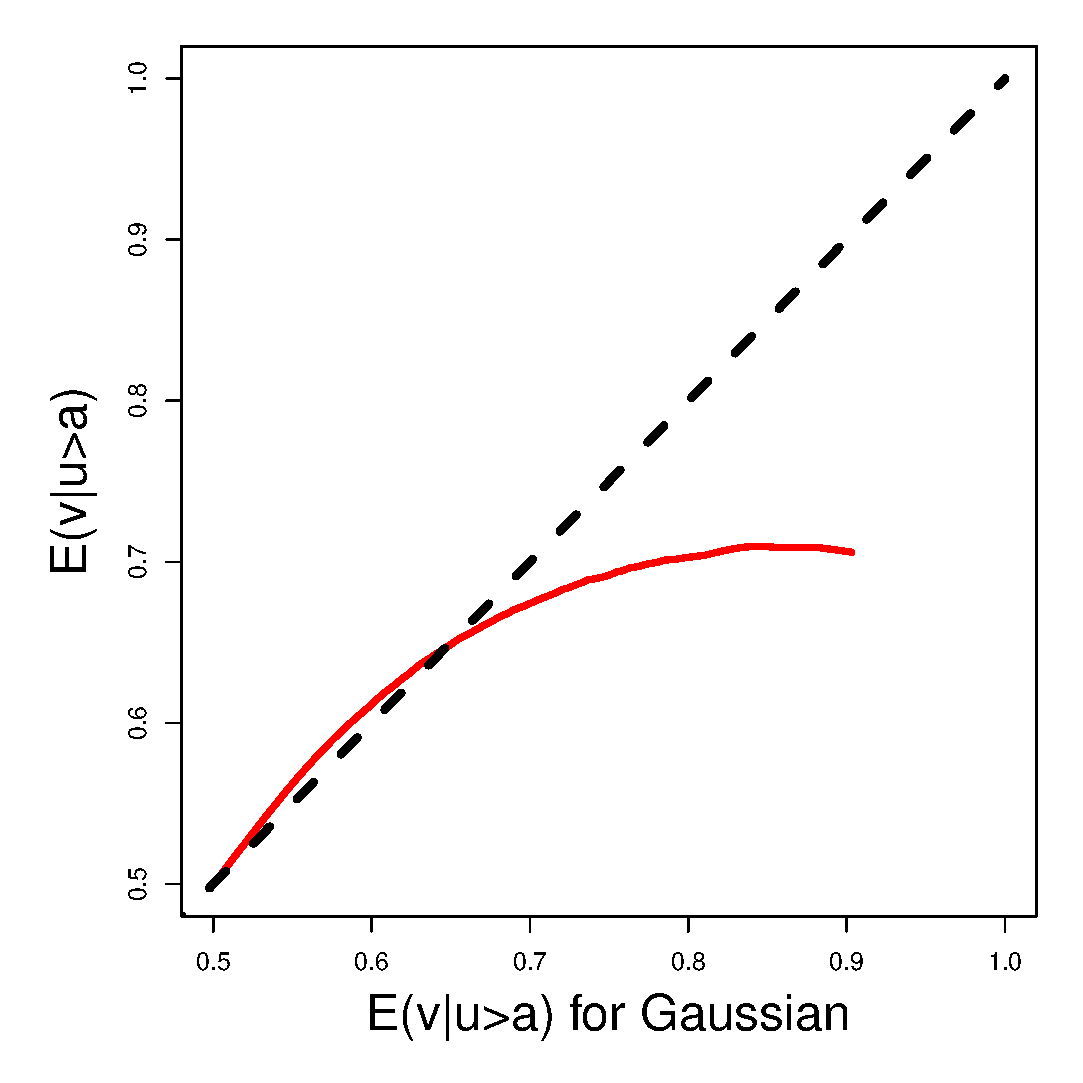
\includegraphics{claytonvs.eps}} \\
            \resizebox{40mm}{!}{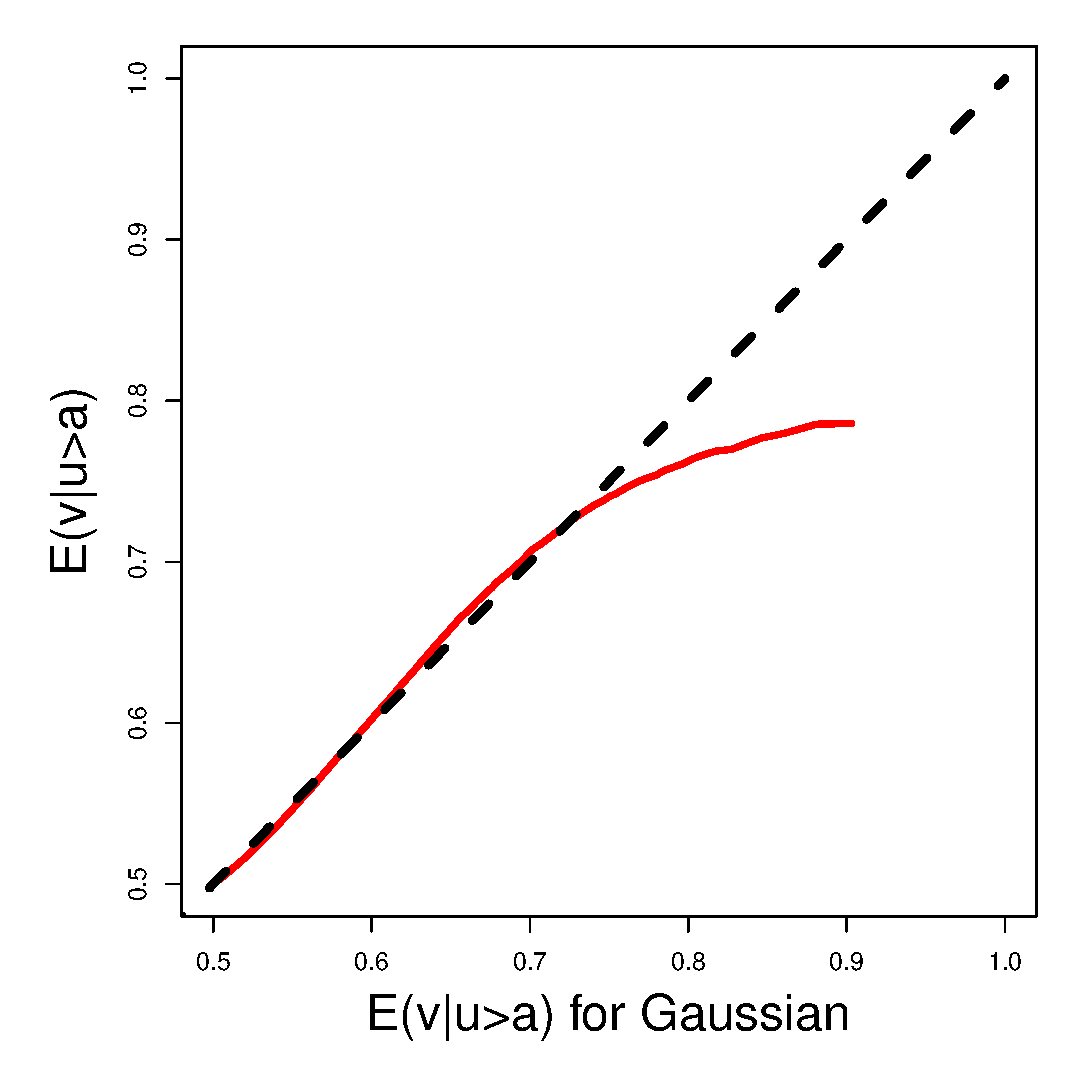
\includegraphics{frankvs.eps}}
            \resizebox{40mm}{!}{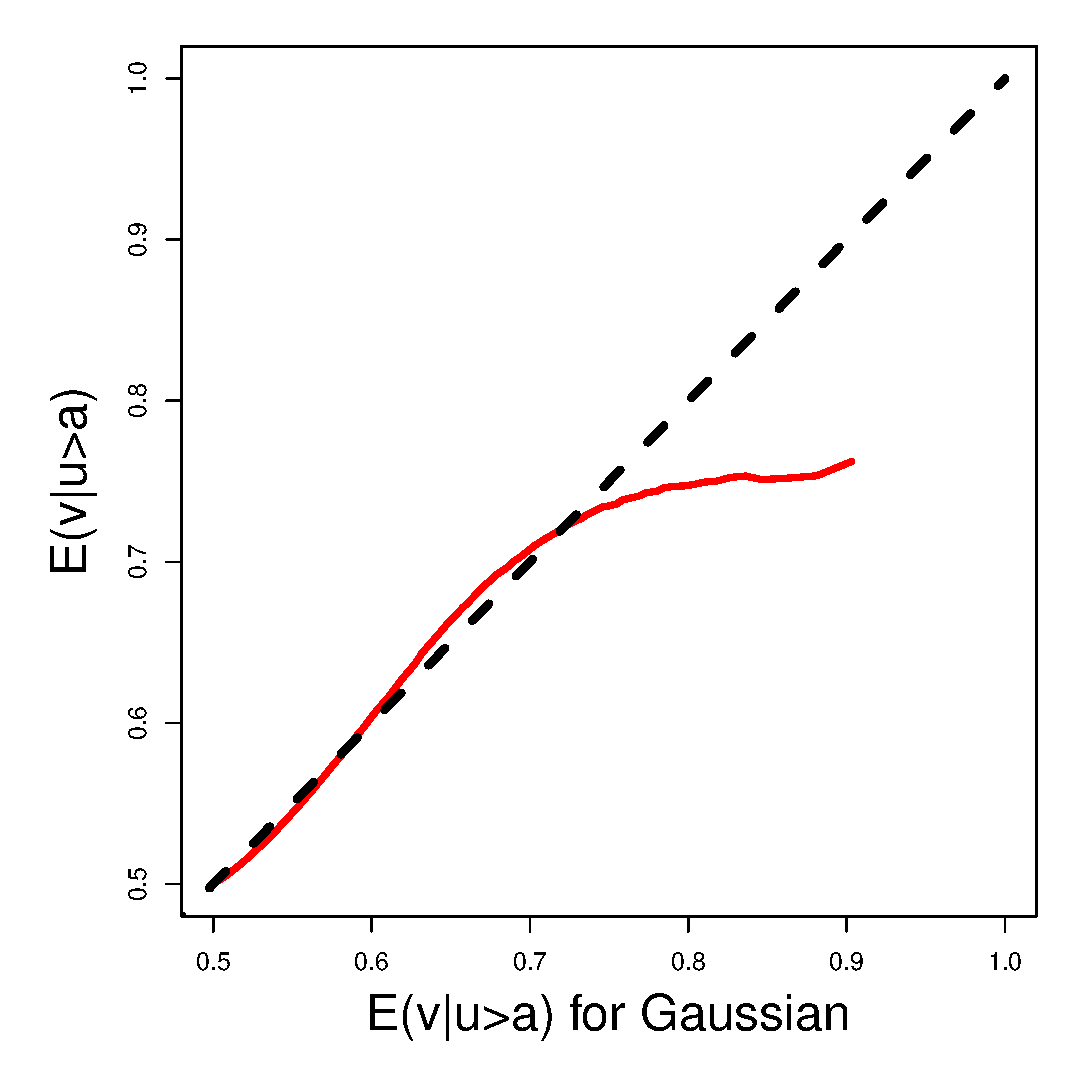
\includegraphics{structural3vs.eps}}
      \resizebox{40mm}{!}{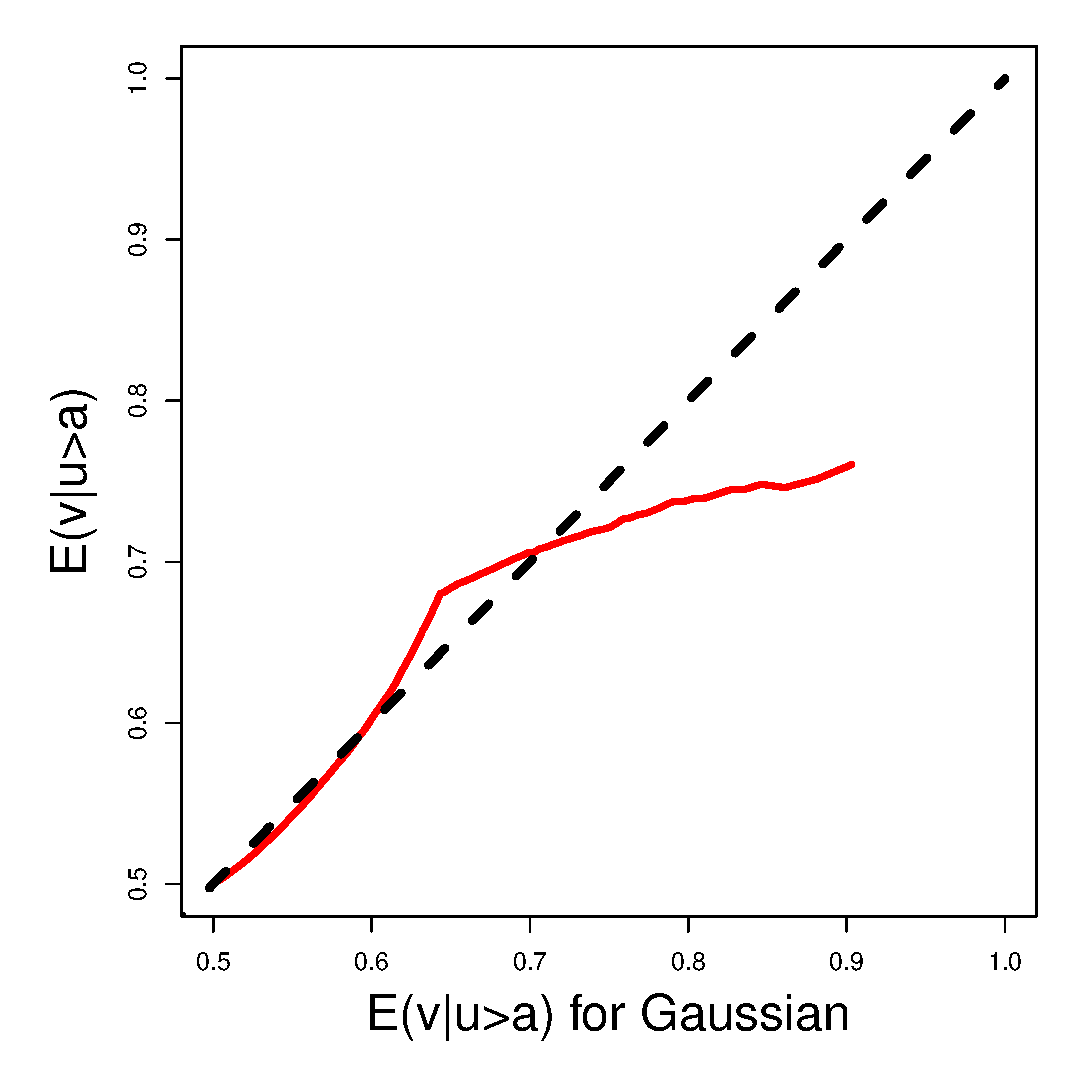
\includegraphics{structural4vs.eps}} \\
    \end{tabular}
    \caption{Plot of upper conditional tail expectations $\E(v|u>\alpha)$ for given copulas against the same for the Gaussian copula.}
    \label{comparison}
  \end{center}
\end{figure}

\fref{fillustration1} expands \fref{fillustration} by graphing layer dependence curves for several parameters of Gaussian, Gumbel, Clayton and Frank copulas. Layer dependence curves summarise essential information (dependence structure) underlying each copula:
\begin{itemize}

\item Gaussian copula: symmetric U-shaped dependence with stronger dependence for larger $\ell$.

\item Gumbel copula: asymmetric U-shaped dependence with stronger dependence for larger $\theta$. Perfect upper tail dependence is always present.

\item Clayton copula: linearly declining dependence with stronger dependence for larger $\theta$. Perfect lower tail dependence is always present.

\item Frank copula: relatively stable dependence with stronger dependence for larger $\theta$.

\end{itemize}
Computing the layer dependence curve is an insightful and important exercise, particularly when the parametric form of a given copula is difficult to interpret, or when the dependence structure underlying an empirical copula is not apparent. Overall dependence measures such as  $\rho_S$ or Kendall's $\tau$ provide information on overall dependence rather than ``local dependence." Section \aref{sliterature} compares layer dependence with existing local dependence measures. It is shown that layer dependence provides a more accurate measure of local dependence. In addition layer dependence possesses coherence properties, further discussed in \sref{scoherence}.

\begin{figure}
  \begin{center}
    \begin{tabular}{cc}
      \resizebox{60mm}{!}{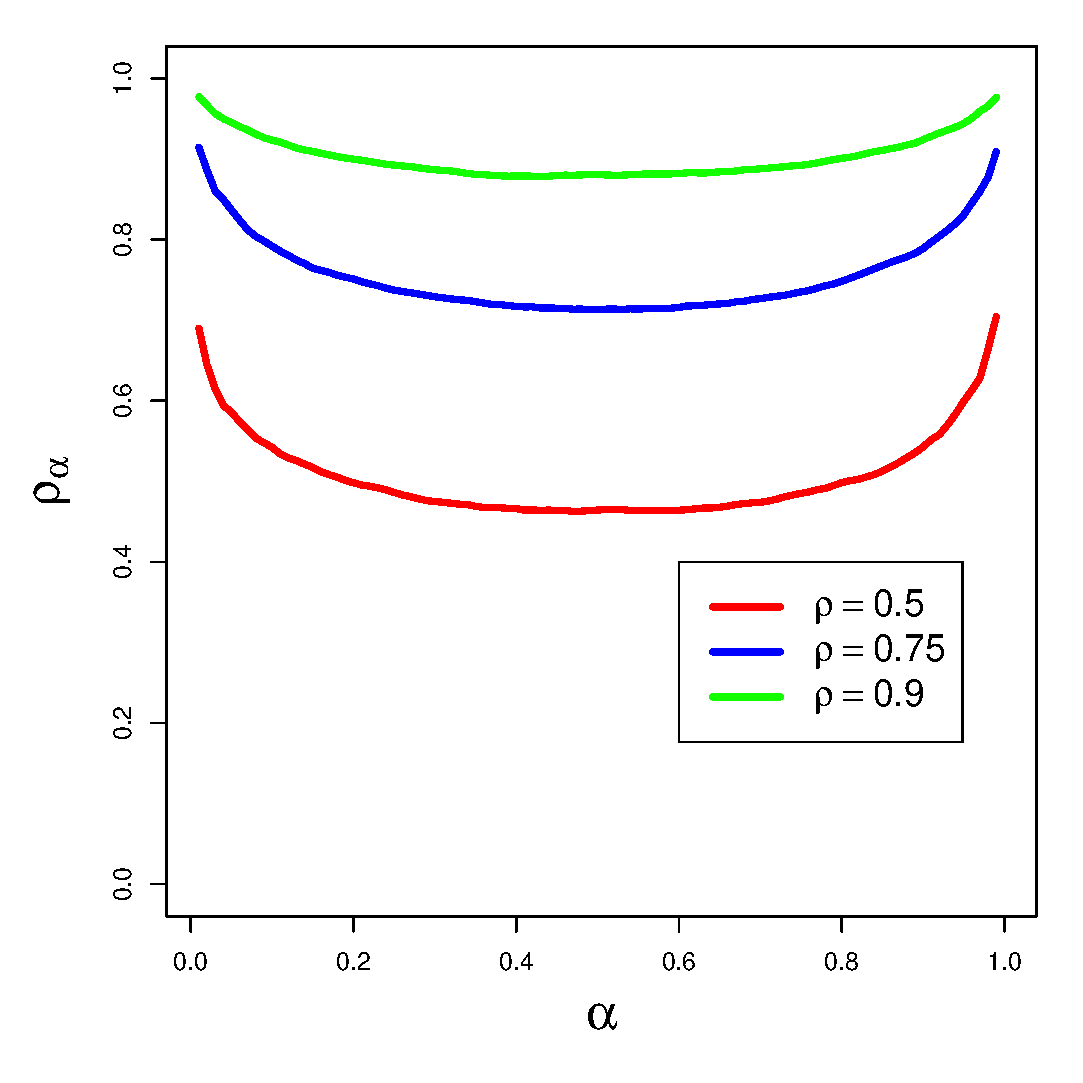
\includegraphics{gaussianmul.eps}}
      \resizebox{60mm}{!}{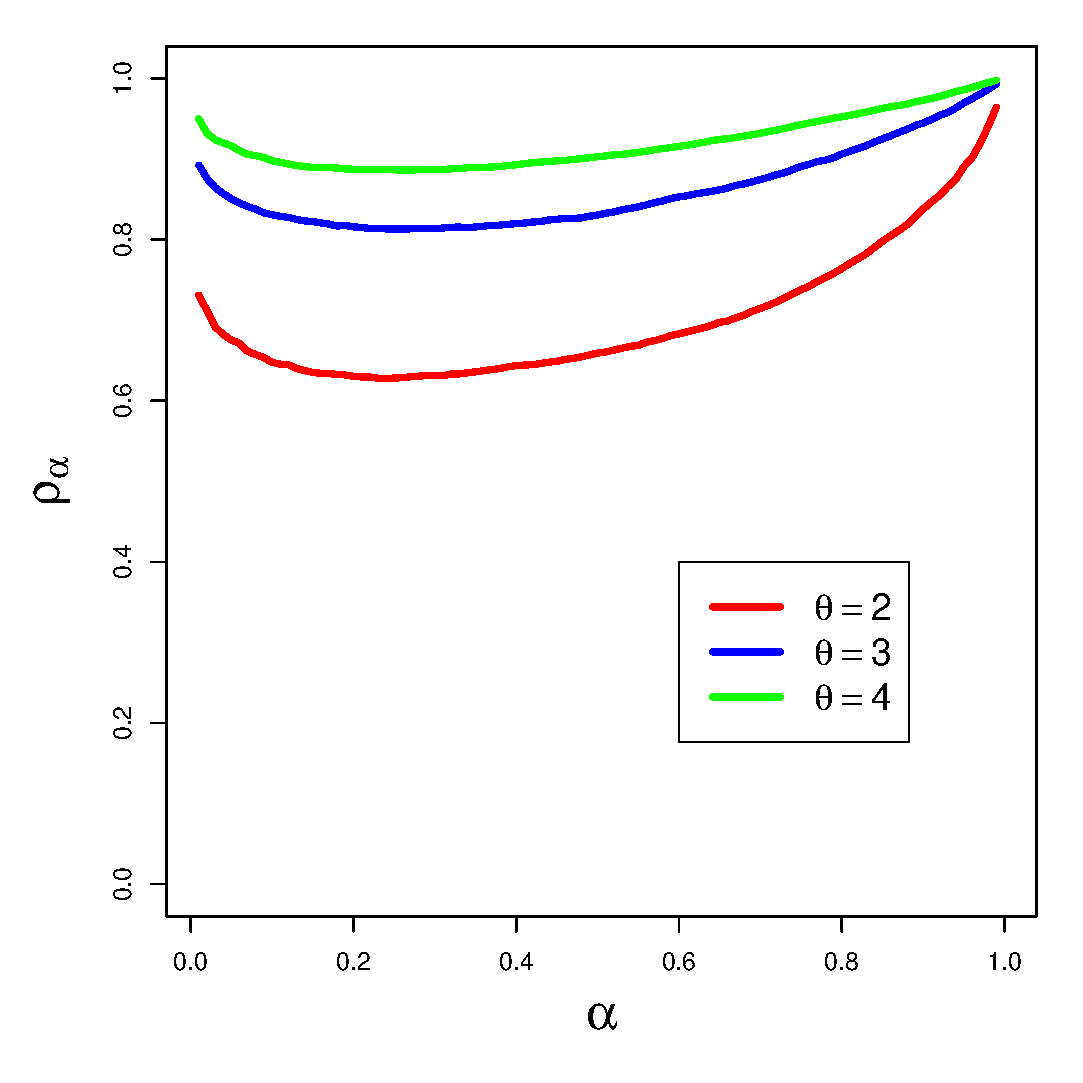
\includegraphics{gumbelmul.eps}} \\
      \resizebox{60mm}{!}{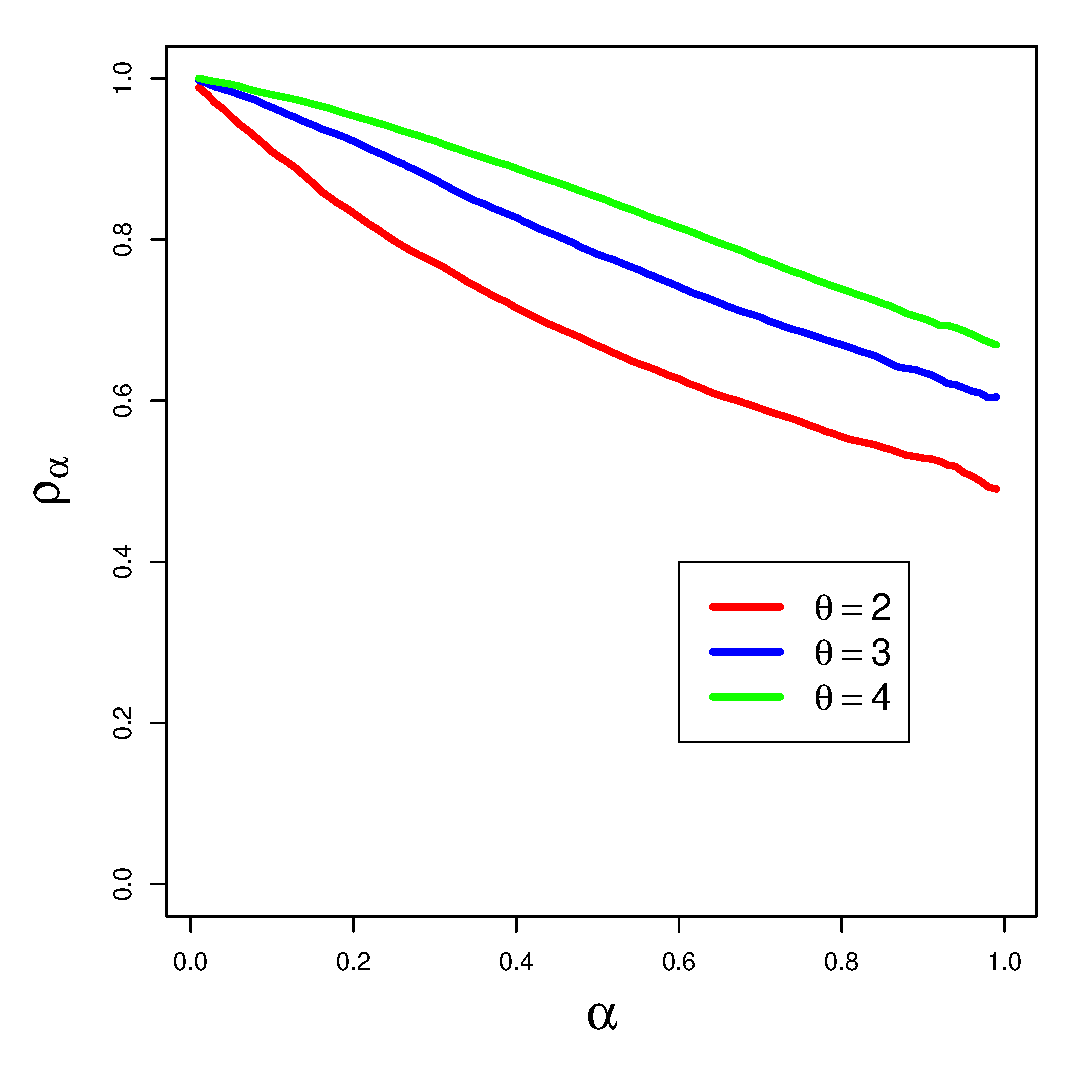
\includegraphics{claytonmul.eps}}
      \resizebox{60mm}{!}{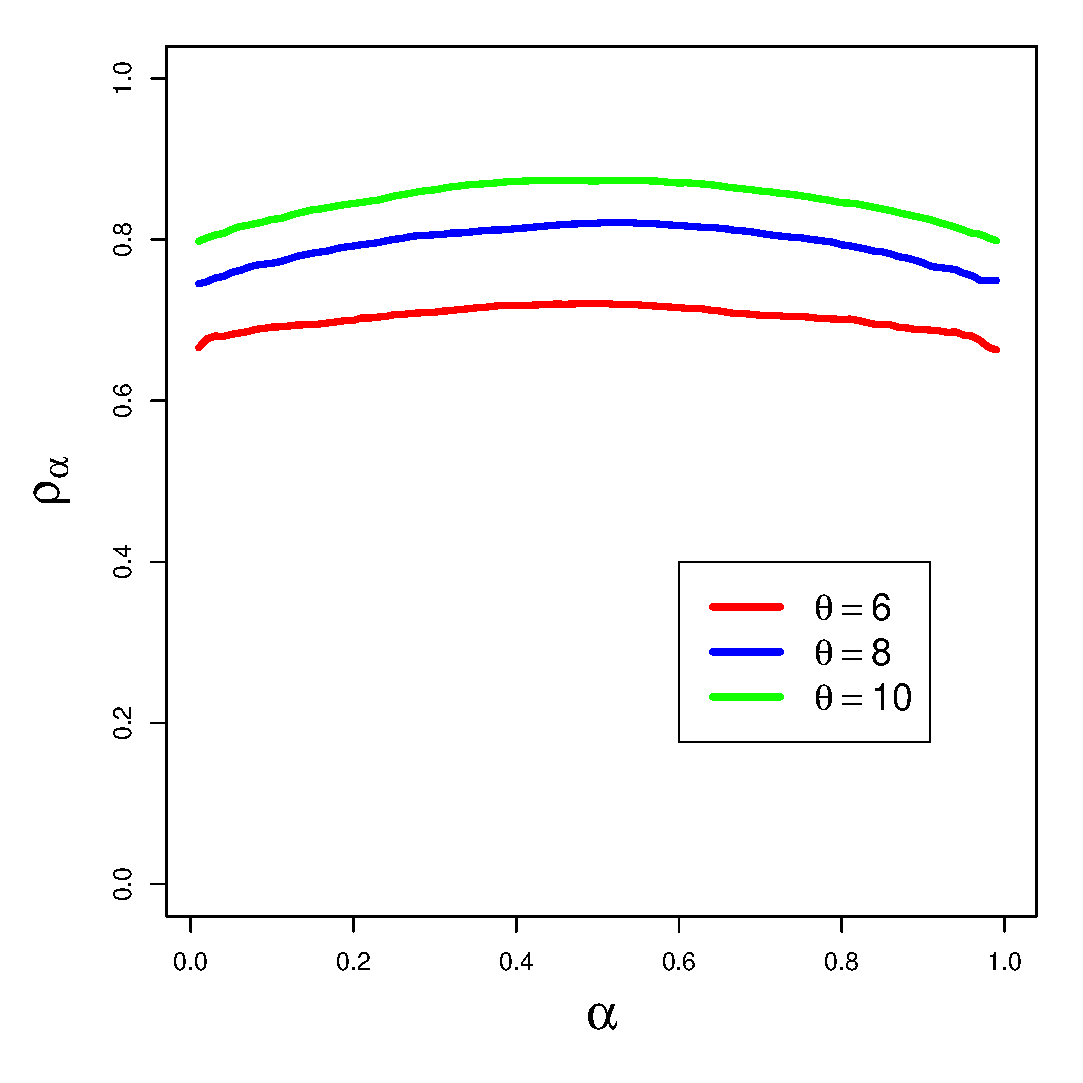
\includegraphics{frankmul.eps}} \\
    \end{tabular}
    \caption{layer dependence curves for various parameters of a Gaussian copula (top left), Gumbel copula (top right), Clayton copula (bottom left) and Frank copula (bottom right). Parameter values are shown in legends.}
    \label{fillustration1}
  \end{center}
\end{figure}





\subsection{``Locality" of layer dependence}

layer dependence $\ell_\alpha$ measures correlation between $u$ in the neighbourhood of $\alpha$ and $v$. This ``locality" property is not apparent from the definition of $\ell_\alpha$. The following is a proof. Define $\ell_{[a,b]}$ as the weighted average
$$
\ell_{[a,b]} \equiv \frac{\int_a^b \ell_\alpha w_\alpha \de \alpha}{\int_a^b w_\alpha \de\alpha}
=\frac{\cov(v,u_{[a,b]})}{\cov(u,u_{[a,b]})}
\cq u_{[a,b]}\equiv \int_a^b (u>\alpha)\de\alpha \;,
$$
where $w_\alpha=6\alpha(1-\alpha)$ and $u_{[a,b]}$ is the ``$[a,b]$ layer" of $u$. Hence the weighted average $\ell_{[a,b]}$ is the scaled correlation between $[a,b]$ layer of $u$ and $v$. Taking the limit $b\rightarrow a^+$ of $\ell_{[a,b]}$ and setting $a=\alpha$ yields $\ell_\alpha$. Rewriting $u_{[a,b]}$ yields
$$
u_{[a,b]}=(u>a)\int_a^{\min(u,b)} \de \alpha = (u>a)\left\{\min(u,b)-a \right\} \;.
$$
Hence the $[a,b]$ layer of $u$ is constant and equal to $0$ when $u\leq a$ and $b-a$ when $u>a$. When $a<u\leq b$, $u_{[a,b]}=u-a$ implying the $[a,b]$ layer of $u$ moves in line with $u$. Therefore the weighted average $\ell_{[a,b]}$ measures correlation between movements of $u$ in the interval $[a,b]$ and $v$. Taking the limit $b\rightarrow a^+$ implies $\ell_\alpha$ measures correlation between $u$ in the neighbourhood of $\alpha$ and $v$. Hence layer dependence measures ``local" dependence.


\subsection{Connection to first-order conditional expectations}

layer dependence in \eref{definition} transforms first order conditional tail expectations into measures of local dependence between $u$ and $v$. Suppose the regression curve of $v$ on $u$, or $\E(v|u=t)$ for all $0\leq t\leq 1$, is given. Then $\alpha$-layer dependence is the integral
$$
\ell_\alpha = 2\left\{\frac{1}{1-\alpha}\int_\alpha^1 \E(v|u=t) \de t - \frac{1}{\alpha}\int_0^\alpha \E(v|u=t) \de t \right\} \;.
$$
Given $\alpha$-layer dependence yields first order conditional expectations:
$$
\E(v|u>\alpha)=\ell_\alpha \E(u|u>\alpha) + 0.5(1-\ell_\alpha)  \;,
$$
$$
\E(v|u=\alpha)=\alpha\ell_\alpha +0.5(1-\ell_\alpha)-0.5\alpha(1-\alpha)\ell'_\alpha \;.
$$
Hence first order conditional expectations are a weighted average of corresponding expectations assuming comonotonicity and independence, with weights $\ell_\alpha$ and $1-\ell_\alpha$, respectively. The conditional expectation $\E(v|u=\alpha)$ requires an additional adjustment term $0.5\alpha(1-\alpha)\ell'_\alpha$ based on the derivative $\ell'_\alpha$.


\end{comment}






\section{Connections to existing measures of tail dependence}\label{sliterature}

Measures have been proposed to capture the degree of tail dependence. Tail dependence is dependence between extreme values of random variables, in this case values of $u$ and $v$ near 0 or 1. Strong tail dependence creates catastrophic events such as  multiple bank failures and  market crashes. Layer dependence is intimately connected to two existing tail dependence measures -- coefficient of tail dependence and tail concentration function. \cite{sweeting2013calculating} and \cite{durante2014copulas} further discusses tail dependence measures.

\subsection{Tail dependence}

\cite{joe1997multivariate} defines coefficients of lower and upper tail dependence in terms of the limiting tail probabilities
 $$
\lambda_L \equiv \lim_{\alpha\rightarrow 0} \p(v\leq \alpha |u\leq \alpha) \cq
\lambda_U \equiv \lim_{\alpha\rightarrow 1} \p(v>\alpha |u>\alpha) \;.
$$
Unit coefficients indicate perfect positive tail dependence, and occur if and only if $u$ and $v$ converge simultaneously to 0 (lower tail) or 1 (upper tail). Coefficients of negative tail dependence replace $v\leq \alpha$ and $v>\alpha$ in the above expressions with $v>1-\alpha$ and $v\leq 1-\alpha$, respectively.  \cite{sweeting2013calculating} discusses the drawback of these coefficients and suggests a modification by weakening the limits, yielding links to tail concentration functions discussed below.

The following shows $\lambda_L=1$ is equivalent to $\ell_0=1$ and $\lambda_U=1$ is equivalent to $\ell_1=1$. Similar links apply to negative tail dependence. Hence \cite{joe1997multivariate} and layer dependence characterise perfect tail dependence equivalently. From \eref{gapexp}, $\ell_1=2\E(v|u=1)-1$ implying $\ell_1=1$ if and only if $\E(v|u=1)=1$.  Hence $\ell_1=1$ if and only if $u=1$ implies $v=1$, which is equivalent to $\lambda_U=1$. In addition $\ell_0=1$ if and only if $u=0$ implies $v=0$, which is equivalent to $\lambda_L=1$. Similar proofs apply to perfect negative tail dependence. 



\subsection{Tail concentration function}

Tail concentration \citep{venter2002tails} is a local dependence measure formed by combining lower and upper conditional tail probabilities at $\alpha$:
$$
\tau_\alpha \equiv (\alpha\leq 0.5) \p(v\leq \alpha|u\leq \alpha) + (\alpha>0.5)\p(v>\alpha|u>\alpha) \;.
$$
Higher tail concentration $\tau_\alpha$ implies $u$ and $v$ are more likely to fall in the same lower tail ($\alpha\leq 0.5$) or upper tail ($\alpha>0.5$). In addition taking the limits $\alpha\rightarrow 0$ or $\alpha\rightarrow 1$ yields coefficients of tail dependence $\lambda_L$ and $\lambda_U$ discussed above. Properties of tail concentration and its applications to distinguish families of copulas are further discussed in \cite{durante2014copulas}.


To display the connection of layer dependence to tail concentration, rewrite the latter  in terms of the copula $C$ of $(u,v)$:
$$
\tau_\alpha = (\alpha\leq 0.5)\frac{C(\alpha,\alpha)}{\alpha}+(\alpha>0.5)\frac{1-2\alpha+C(\alpha,\alpha)}{1-\alpha} \;.
$$
Standardising $\tau_\alpha$ by subtracting the value under independence and dividing by the departure from independence under comonotonicity yields
$$
\tau_\alpha^* \equiv \frac{\tau_\alpha - \{\alpha(\alpha\leq 0.5)+(1-\alpha)(\alpha>0.5)\}}{1-\{\alpha(\alpha\leq 0.5)+(1-\alpha)(\alpha>0.5)\}}
=\frac{C(\alpha,\alpha)-\alpha^2}{\alpha(1-\alpha)} = -\gamma_\alpha \;,
$$
where $\gamma_\alpha$ is defined below \eref{decomposition}.

Hence, using \eref{decomposition}, $\ell_\alpha=1-2\delta_\alpha(1-\tau_\alpha^*)$ where $\delta_\alpha$ is the average dispersion between points $(u,v)$ discordant at $\alpha$. Note $\ell_\alpha$ and $\tau_\alpha^*$ have the same sign. Hence layer dependence refines tail concentration by standardising it and including further information on dispersion.


\section{Further properties of layer dependence}\label{sproperties}

This section lists and explores further properties and results of layer dependence.




\subsection{Copula integration}

Layer dependence $\ell_\alpha$ can be written as a standardised integral of the copula 

\begin{equation}\label{copula}
\ell_\alpha = \frac{\int_0^1 \cov\{I_\alpha(u),I_\beta(v)\} \de\beta }{\alpha(1-\alpha)/2}
= \frac{2 \int_0^1 C(\alpha,\beta) \de \beta- \alpha}{\alpha(1-\alpha)} \;.
\end{equation}
Note $\cov\{(u>\alpha),(v>\beta)\}=C(\alpha,\beta)-\alpha\beta$ and apply \eref{decompose} to $v$, to derive

Thus $\ell_\alpha$ integrates copulas to reduce their dimension from two and one, and scales the result to ensure it lies between $\pm 1$.

With Archimedean copulas \citep{mcneil2005qrm} $C(\alpha,\beta) =\psi^-\left\{\psi(\alpha)+\psi(\beta)\right\}$ where $\psi$ is the generator function and $\psi^-$ its inverse. In this case closed form expressions for the integrals and hence for $\ell_\alpha$ do not exist.



\subsection{Layer dependence preserves convex combination}

A direct consequence of the copula integration result \eref{copula} is layer dependence preserves convex combinations of random variables, as follows.

Suppose $(u^*,v^*)$ is bivariate uniform with $\alpha$--layer dependence $\ell_\alpha^*$ and copula $C^*$. Then a convex combination of $(u,v)$ and $(u^*,v^*)$ yielding the copula $\pi C+(1-\pi)C^*$ where $0\le \pi\le 1$ is constant has layer dependence $\pi\ell_\alpha+(1-\pi)\ell_\alpha^*$. The proof follows directly from \eref{copula}.

This result generalises to multiple and continuous convex combinations of bivariate uniform random variables and their copoulas. 



\subsection{One-sided conditional tail expectations}


Since $\E(v)=\alpha\E(v|u\leq \alpha)+(1-\alpha)\E(v|u>\alpha)$ it is straightforward to show from \eref{gapexp} that
$$
\ell_\alpha = \frac{\E(v|u> \alpha)-\E(v)}{\E(u|u> \alpha)-\E(u)} = \frac{\E(v|u\leq \alpha)-\E(v)}{\E(u|u\leq \alpha)-\E(u)} \;,
$$
the gap between upper or lower conditional tail expectations of $v$ and the unconditional expectation. Denominators are again scaling factors ensuring $\ell_\alpha=1$ if $u$ and $v$ are comonotonic and $\ell_\alpha=-1$ if countermonotonic.

\begin{comment}
Rewriting conditional tail expectations in \eref{gapexp} in terms of ``pointwise" conditional expectations yields
$$
\ell_\alpha = 2\left\{\frac{1}{1-\alpha}\int_\alpha^1 \E(v|u=t) \de t - \frac{1}{\alpha}\int_0^\alpha \E(v|u=t) \de t \right\} \;,
$$
hence $\alpha$-layer dependence is the difference between average points on the regression curve of $v$ on $u$ over $u>\alpha$ and $u\leq\alpha$.
\end{comment}



\subsection{Layer dependence does not uniquely characterise a copula}


Layer dependence curves extract and summarise dependence information in a copula. Therefore layer dependence curves do not uniquely specify the copula, as shown in the following counterexample.

Suppose $v=u$ and $v=1-u$ with equal probability. The former and latter imply layer dependence of $=1$ and $-1$, respectively. Hence $\ell_\alpha=0$ for all $\alpha$ since layer dependence preserves convex combinations as discussed above. The copula of $(u,v)$ is $C(u,v)=0.5\{\min(u,v)+\max(u+v-1,0)\}$. However $\ell_\alpha=0$ is also the case if $u$ and $v$ are independent: $C(u,v)=uv$. Hence layer dependence curves are not unique to the copula.

Non-uniqueness is seen from another perspective using \eref{gapexp}: $\ell_\alpha$ only captures first-order conditional tail expectations. Hence two copulas with equal first-order conditional tail expectations have equal layer dependence.

\begin{comment}

\subsection{Non-exchangeability}

layer dependence retains coherence and dependence-measuring properties when the joint distribution of $(u,v)$ is non-exchangeable. However the calculation of layer dependence differs according to the conditioning variable:
$$
2\left\{\E(v|u>\alpha)-\E(v|u\leq \alpha)\right\} \neq
2\left\{\E(u|v>\alpha)-\E(u|v\leq \alpha)\right\} \;.
$$
The left expression measures local dependence with respect to $u$. The right expression measures local dependence with respect to $v$, and is not necessarily equal to the left. A similar concept applies in regression, where the regression coefficient depends on the assignment of explanatory and dependent variables.

\end{comment}




\subsection{Layer dependence for a non-exchangeable copula}

If $u$ and $v$ are exchangeable, such as in Archimedean copulas \citep{mcneil2005qrm}, then layer dependence is invariant when $u$ and $v$ are switched:
$$
\frac{\cov\{v,(u>\alpha)\}}{\cov\{u,(u>\alpha)\}}
=\frac{\cov\{u,(v>\alpha)\}}{\cov\{v,(v>\alpha)\}} \cq 0\le\alpha\le 1\;.
$$ 
Hence it does not matter whether $u$ or $v$ is decomposed into layers.
 
If $u$ and $v$ are not exchangeable then layer dependence differs when layers of $v$ instead of $u$ are applied, that is dependence between $v$ and $\alpha$--layer of $u$ differs from dependence between $u$ and $\alpha$--layer of $v$.

An analogous property applies to least squares regression: regressing $v$ on $u$ is the same as  regressing $u$ on $v$, if the joint distribution is  exchangeable. The two regressions differ otherwise.










\section{Alternate measures of overall dependence}\label{saltoverall}


Equation \eref{wtdaverage} expresses Spearman's $\rho$ as a weighted average of  $\ell_\alpha$ over $0\le\alpha\le 1$ using weights $w_\alpha=6\alpha(1-\alpha)$ integrating to 1. As mentioned below \eref{wtdaverage}, $w_\alpha$ may be inappropriate since it dismisses tail dependence. Averaging $\ell_\alpha$ using different weights $w^*_\alpha$ yields alternate measures of overall rank dependence:
$$
\rho^*\equiv  \int_0^1 w^*_\alpha \ell_\alpha \de \alpha = \int_0^1 w^*_\alpha \frac{ \cov\{v,(u>\alpha)\}}{\cov\{u,(u>\alpha)\}} \de \alpha=\cov\{W^*(u),v\} \;,
$$
where
$$
W^*(u)\equiv 2\int_0^u \frac{w^*_\alpha}{\alpha(1-\alpha)}\de\alpha \;,
$$
is the weighted cumulative of $w^*_\alpha$. Hence the alternate $\rho^*$ is also a covariance, between $v$ and a transformation of $u$.  For Spearman's $\rho$, $w^*_\alpha=6\alpha(1-\alpha)$ thus $W^*(u)=12u$ yielding $\rho^*=\cov(12u,v)=\cor(u,v)=\rho$. Weights $w^*_\alpha$ indicate the importance of local dependence at various layers of $u$.

Since $\rho^*$ averages $\ell_\alpha$, coherence properties of layer dependence described in section \aref{scoherence} apply to $\rho^*$ for any $0\le w^*_\alpha\le 1$ integrating to one. These properties are $-1\le\rho^*\le 1$,  $\rho^*=-1$, $0$ and $1$ under countermonotonicity, independence and comonotonicity, respectively, $\rho^*$ switching its sign when $u$ or $v$ is replaced by its complement, and higher $\rho^*$ when the correlation order of $(u,v)$ increases.
Identical properties apply to Spearman's $\rho$.

The following are examples of $w_\alpha^*$ yielding rank dependence measures alternate to Spearman's $\rho$:
\begin{itemize}

\item Suppose dependence at different percentiles are equally important.   Then $w^*_\alpha$ is uniform yielding
$$
\rho^*_1 =2\cov\left\{v,\log\left(\frac{u}{1-u}\right)\right\}
= \sqrt{\frac{2}{3}}\ \cor\left\{v,\log\left(\frac{u}{1-u}\right)\right\} \;,
$$
\begin{comment}
\int_0^1 \frac{\cov\{v,(u>\alpha)\}}{\cov\{u,(u>\alpha)\}} \de \alpha
=\cov\left[v,\int_0^1 \frac{(u>\alpha)}{\cov\{u,(u>\alpha)\} }\de \alpha\right]
$$
$$
=\cov\left\{v,\int_0^u \frac{1}{0.5\alpha(1-\alpha) }\de \alpha\right\}
\end{comment}
a multiple of the correlation between $v$ and the logit of $u$. If tail dependence is pronounced, $\rho_1^*>\rho$ since $\rho^*_1$ weights tail dependence more heavily compared to $\rho$. An illustration is shown below.

\item If $w^*_\alpha=3\alpha^2$  then dependence at higher percentiles are considered more important. This formulation is applicable when upper tail dependence is critical, for example the simultaneous occurrence of large insurance losses in different lines of business. Then
$$
\rho_2^* = 6\cov\left\{v,\log\left(\frac{\e^{-u}}{1-u}\right) \right\}
=\sqrt{3} \cor\left\{v,-\log(1-u)\right\}-\frac{\rho}{2}\;.
$$
If dependence is higher over percentiles above the median then $\rho_2^*>\rho$.

\item If dependence over percentiles below the median is more important then for example  $w^*_\alpha=3(1-\alpha)^2$ yielding
$$
\rho_3^* = 6\cov\left\{v,\log \left( u \e^{-u}\right) \right\}
= \sqrt{3}\cor(v,\log u )-\frac{\rho}{2}  \ .
$$


\item Suppose $w^*_\alpha$ is derived from $V_\alpha$, the inverse marginal distribution of $x$ with derivative $V_\alpha'$:
$$
w^*_\alpha = \frac{\cov\{u,(u>\alpha)\}V_\alpha'}{\int_0^1 \cov\{u,(u>\alpha)\}V_\alpha' \de\alpha}
=\frac{\alpha(1-\alpha)V_\alpha'}{\cov(V_u,u)}
=\frac{\alpha(1-\alpha)V_\alpha'}{\cov(x,u)} \;,
$$
where $x=V_u$. This yields the Gini correlation  \citep{schechtman1999proper}
$$
\rho_3^*=\frac{\cov(V_u,v)}{\cov(V_u,u)} = \frac{\cov\{x,G(y)\}}{\cov\{x,F(x)\}} \;,
$$
where $F\equiv V^-$ and $G$ are distribution functions of $x$ and $y$, respectively.  In this example the weights $w^*_\alpha$ depend on the marginal distribution of $x$. More skewness in $x$ leads to more steeply increasing $w^*_\alpha$ hence greater emphasis on upper tail dependence.

\end{itemize}


\subsection{Illustration of alternates to Spearman's $\rho$}


\fref{falternate} illustrates the first three proposed alternates to Spearman's $\rho$ listed above. \fref{falternate} reuses the nine copulas in \fref{fillustration} with equal Spearman's $\rho=0.6$. Spearman's $\rho$ summarises lower and upper dependence symmetrically and dismisses tail dependence. These drawbacks are addressed by the alternate measures. 


For example xxx...




\begin{figure}
  \begin{center}
    \begin{tabular}{ccc}
      \resizebox{40mm}{!}{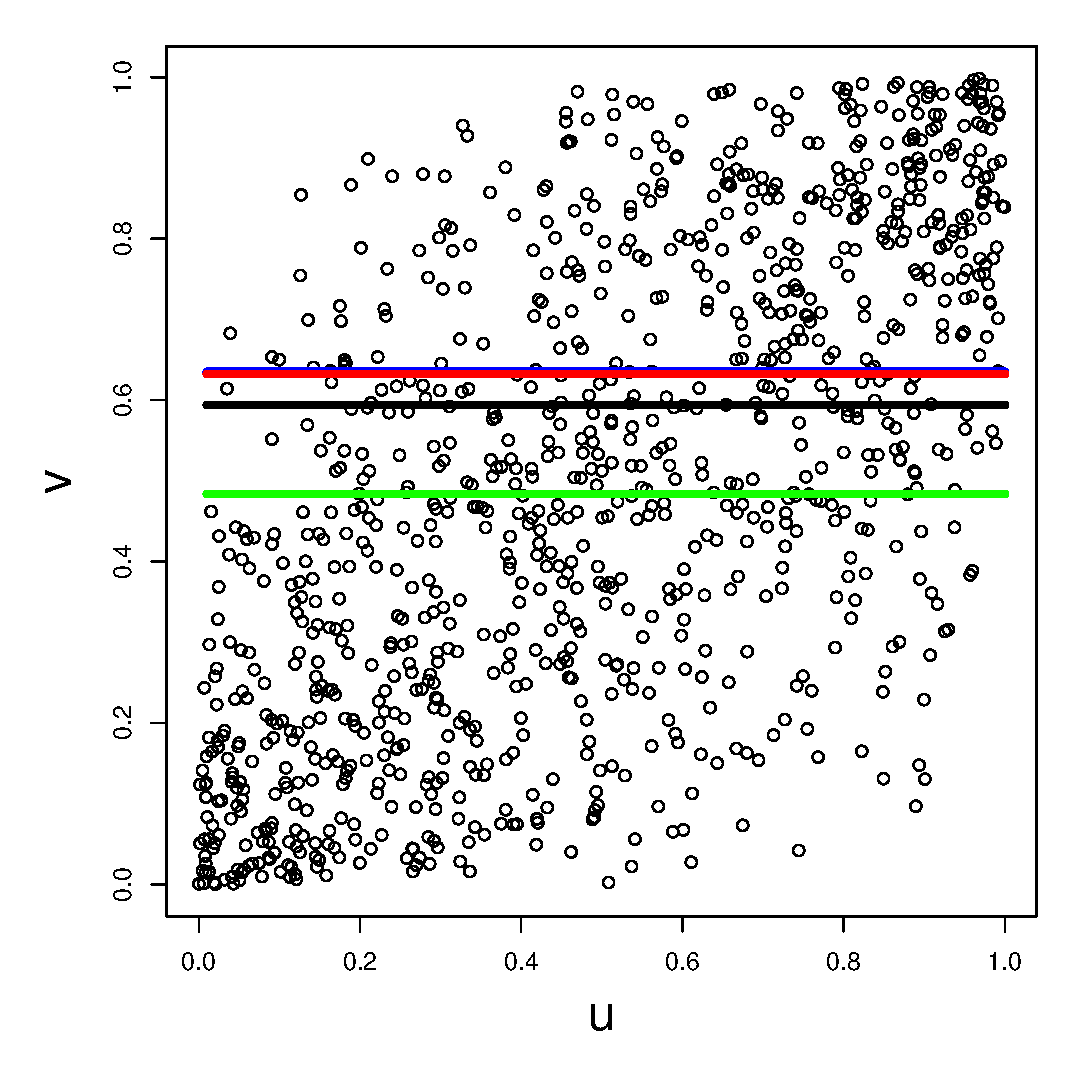
\includegraphics{normal1.eps}}
            \resizebox{40mm}{!}{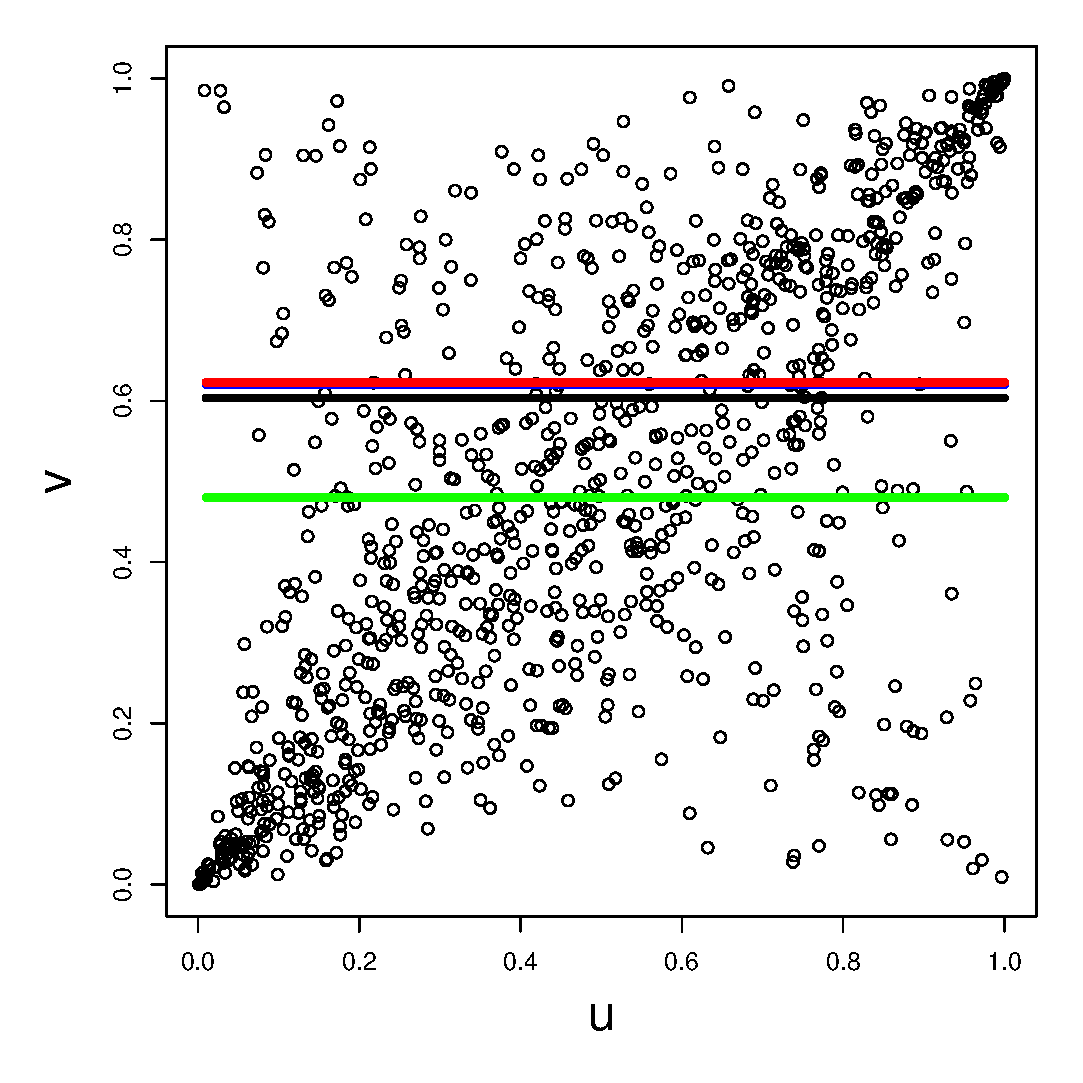
\includegraphics{student1.eps}}
      \resizebox{40mm}{!}{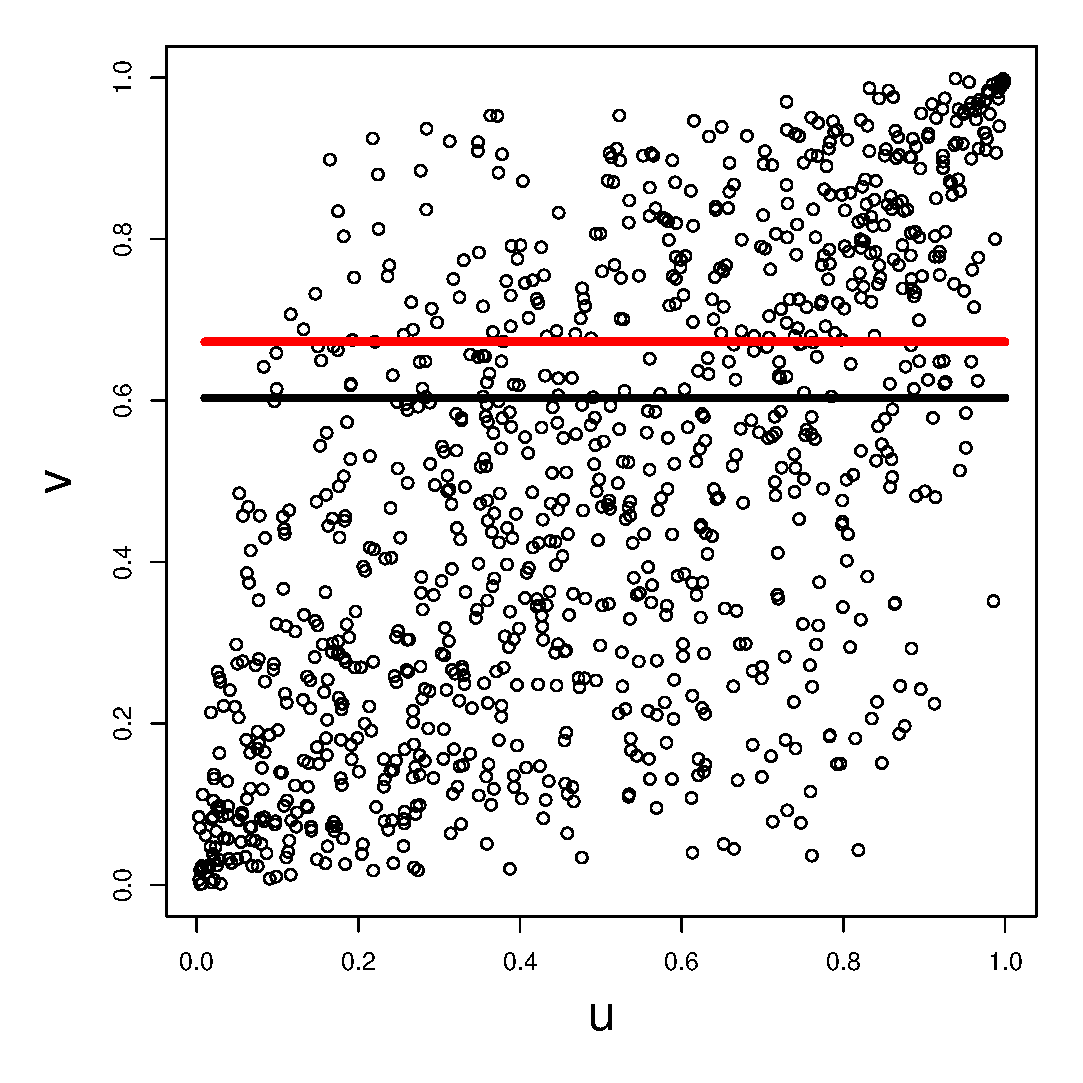
\includegraphics{structural21.eps}} \\
      \resizebox{40mm}{!}{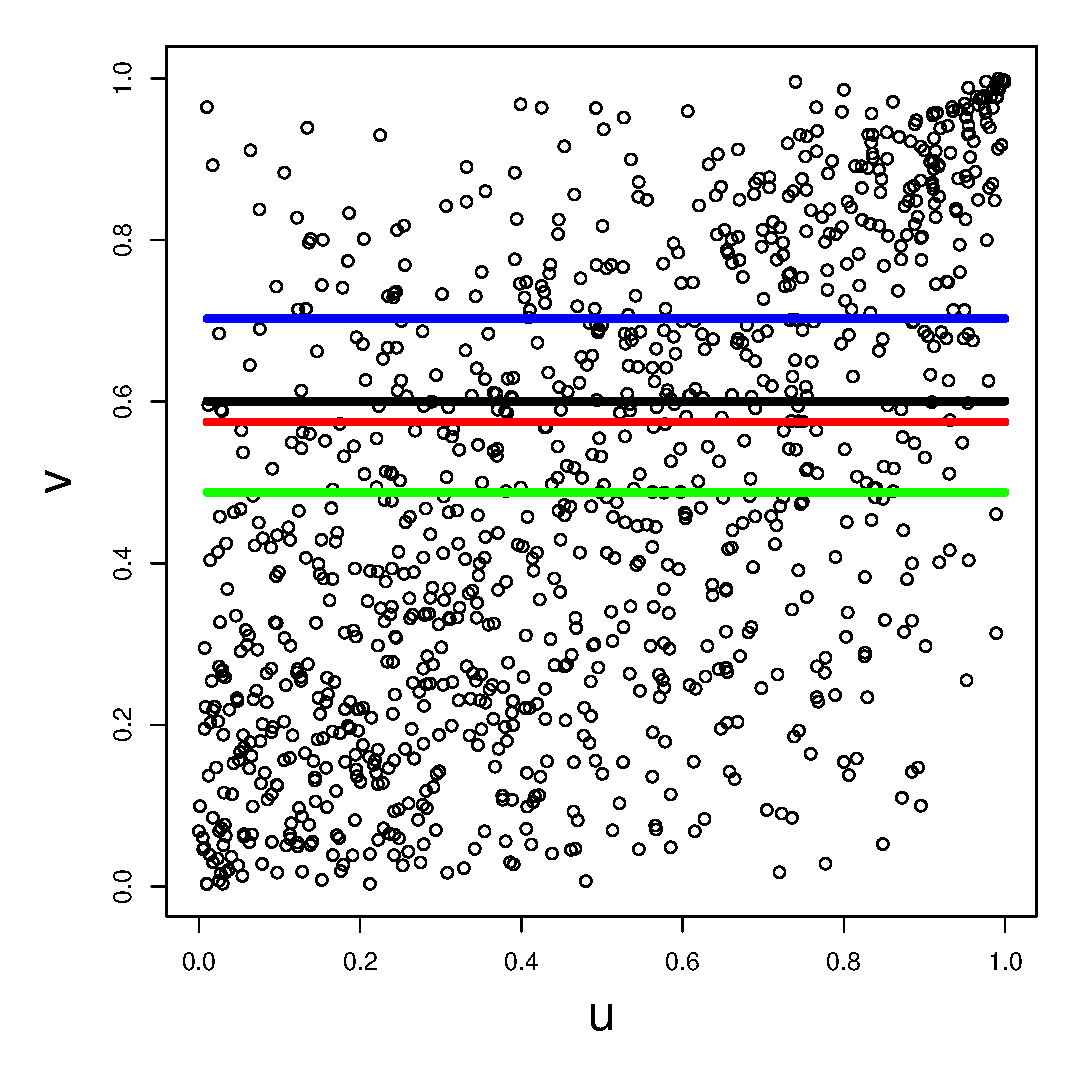
\includegraphics{gumbel1.eps}}
            \resizebox{40mm}{!}{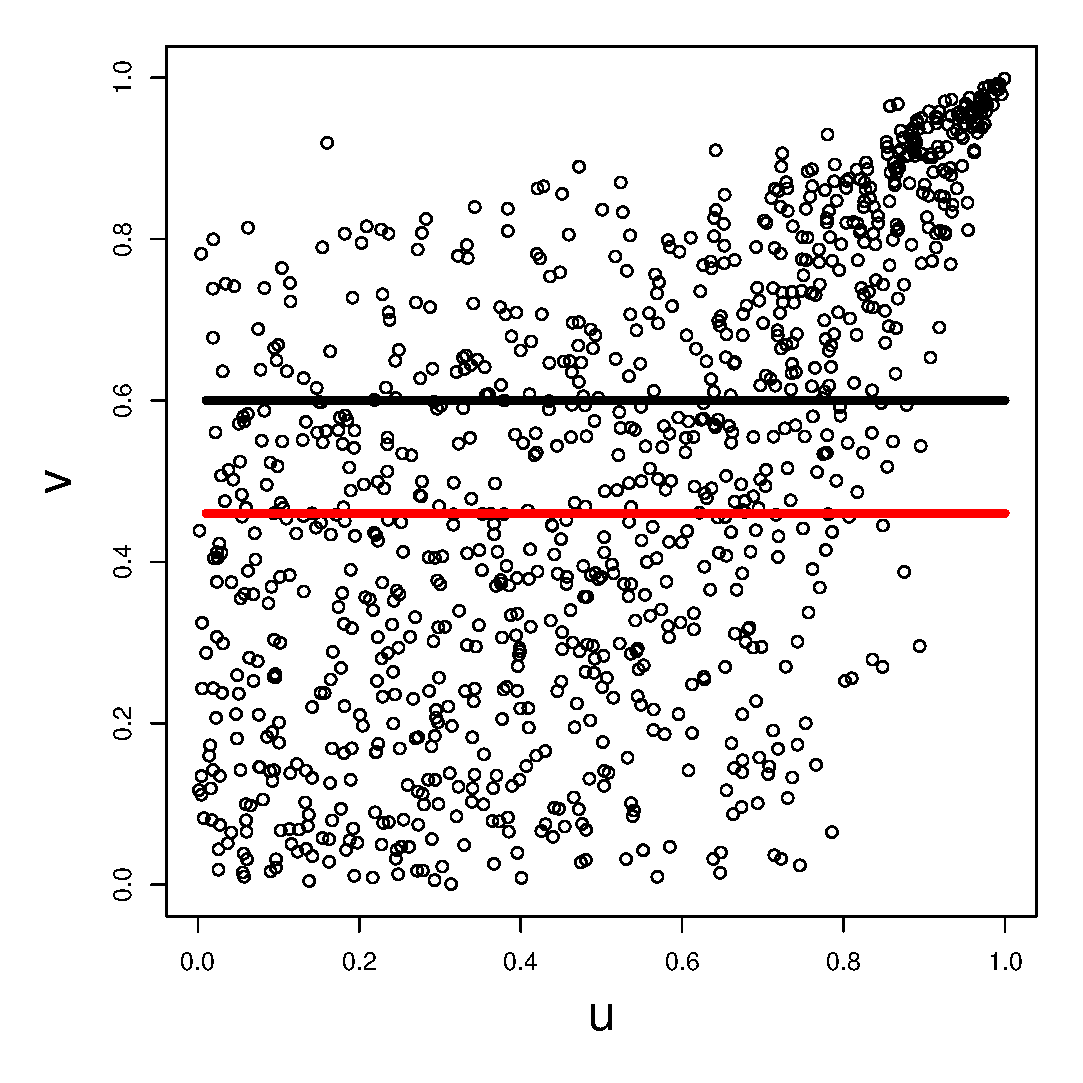
\includegraphics{structural11.eps}}
      \resizebox{40mm}{!}{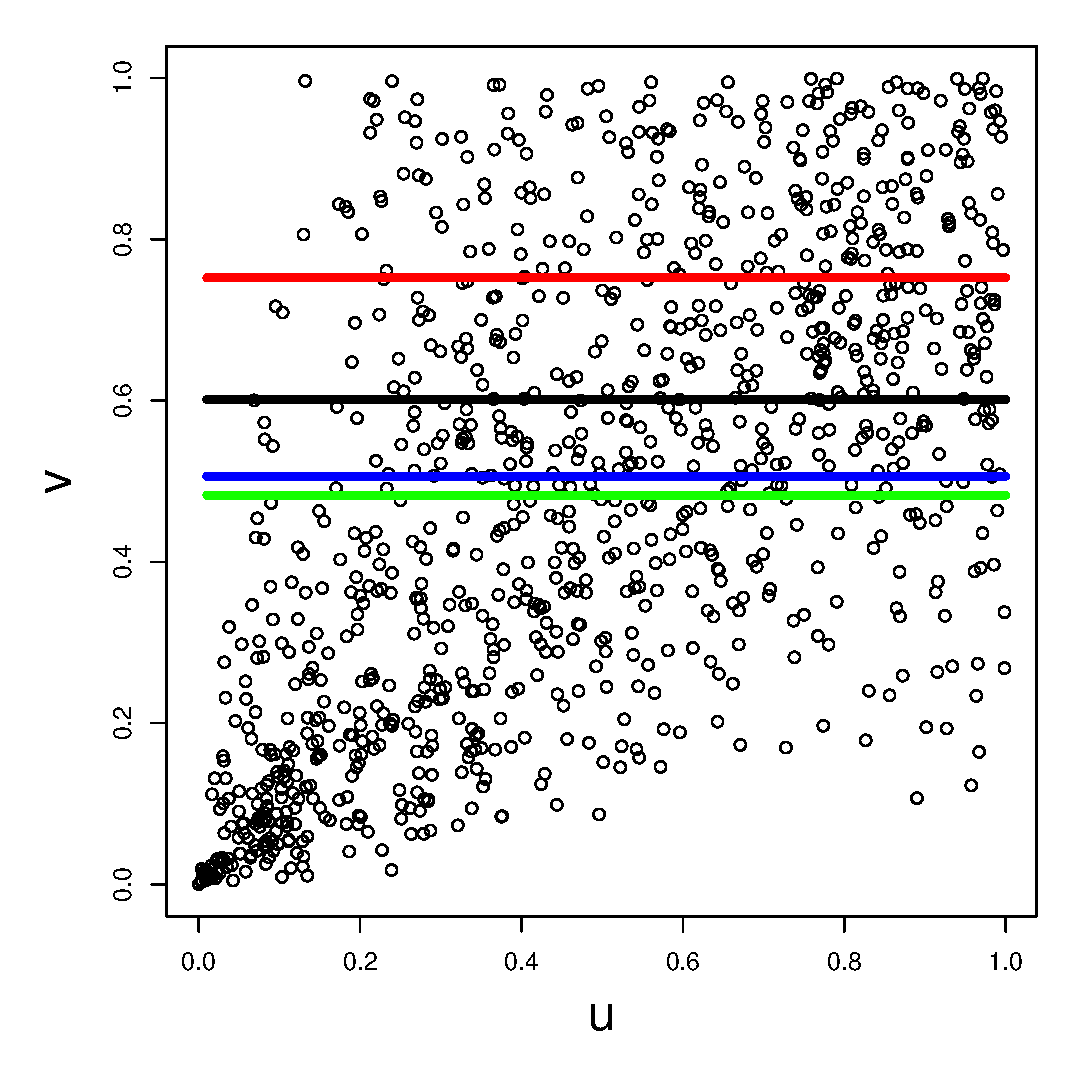
\includegraphics{clayton1.eps}} \\
            \resizebox{40mm}{!}{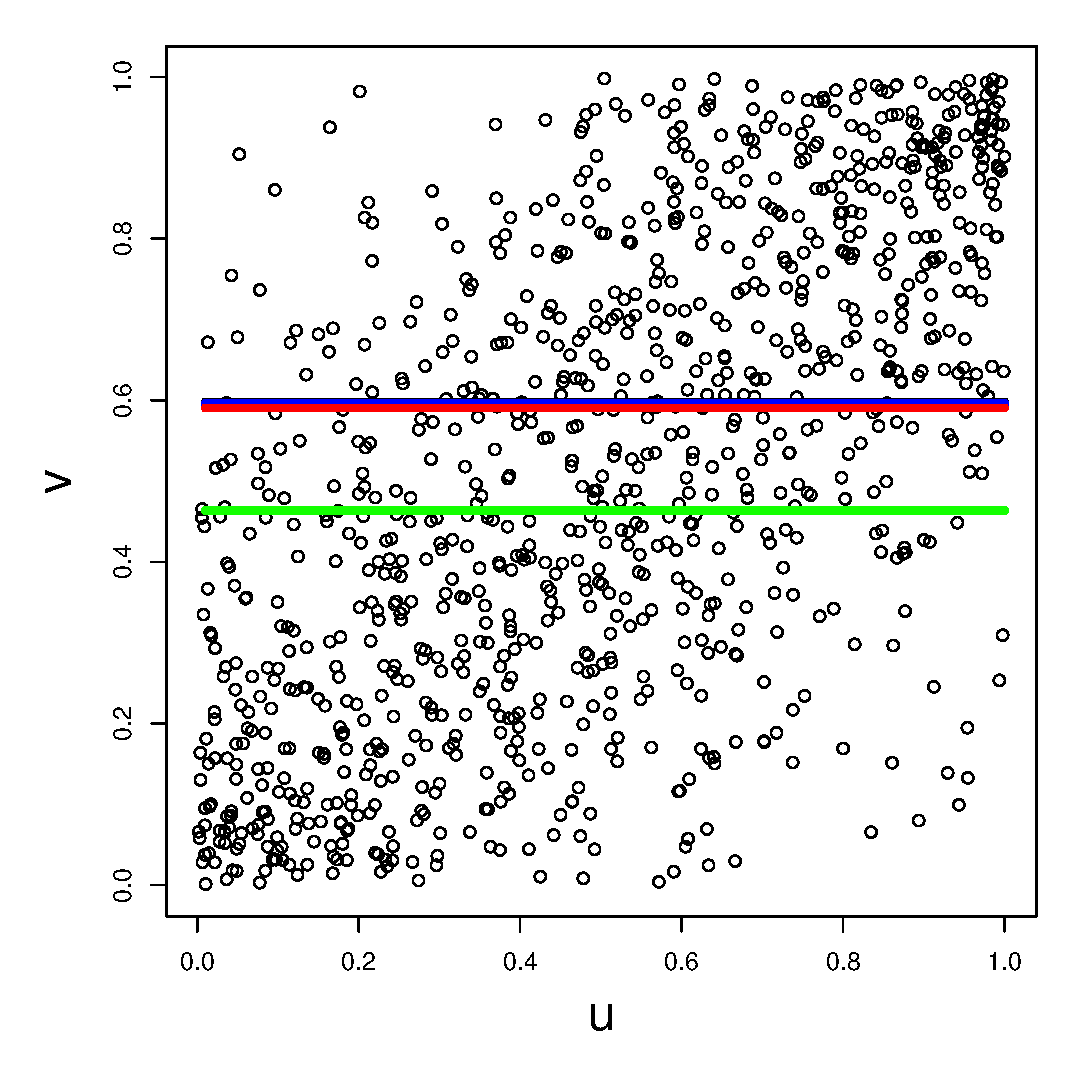
\includegraphics{frank1.eps}}
            \resizebox{40mm}{!}{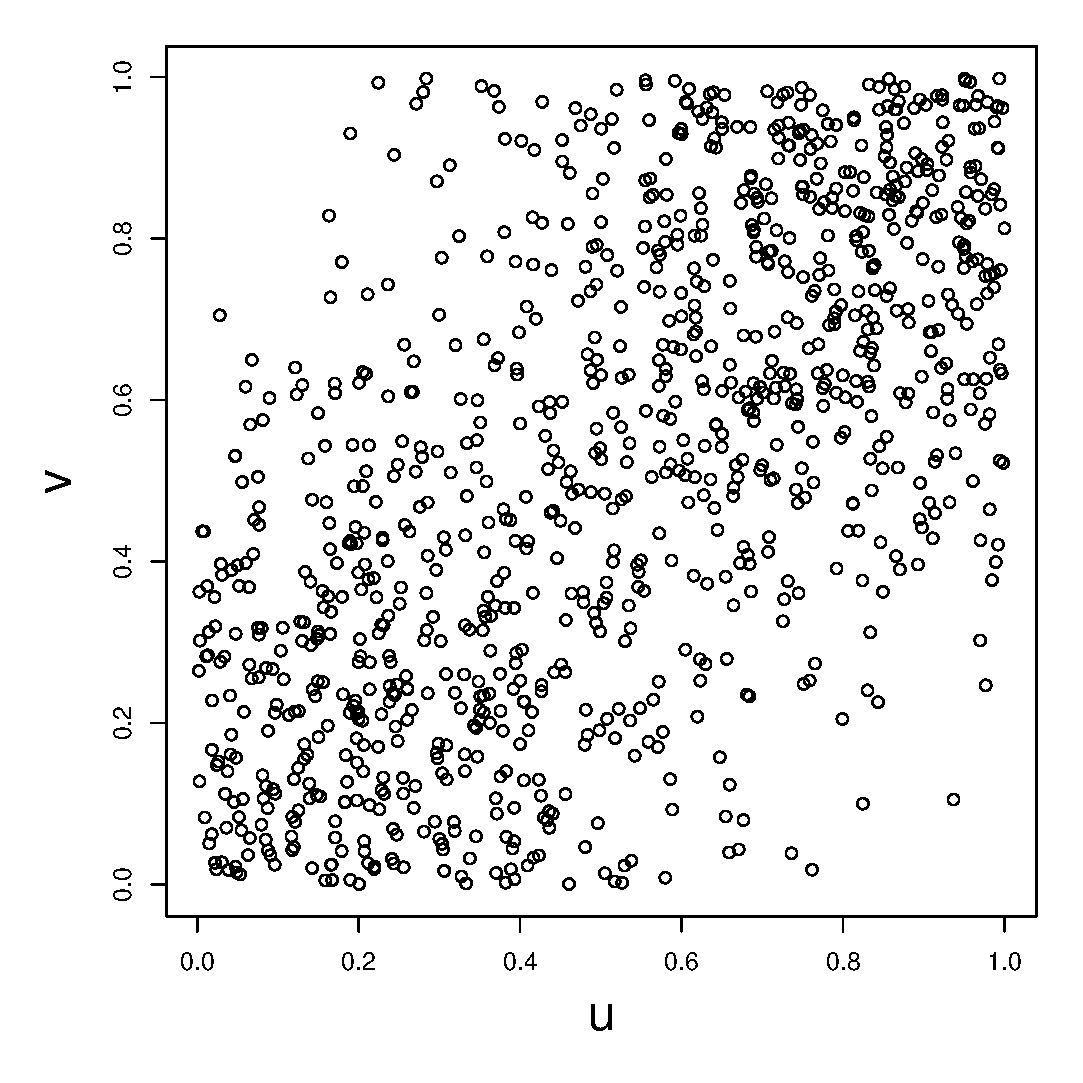
\includegraphics{structural31.eps}}
      \resizebox{40mm}{!}{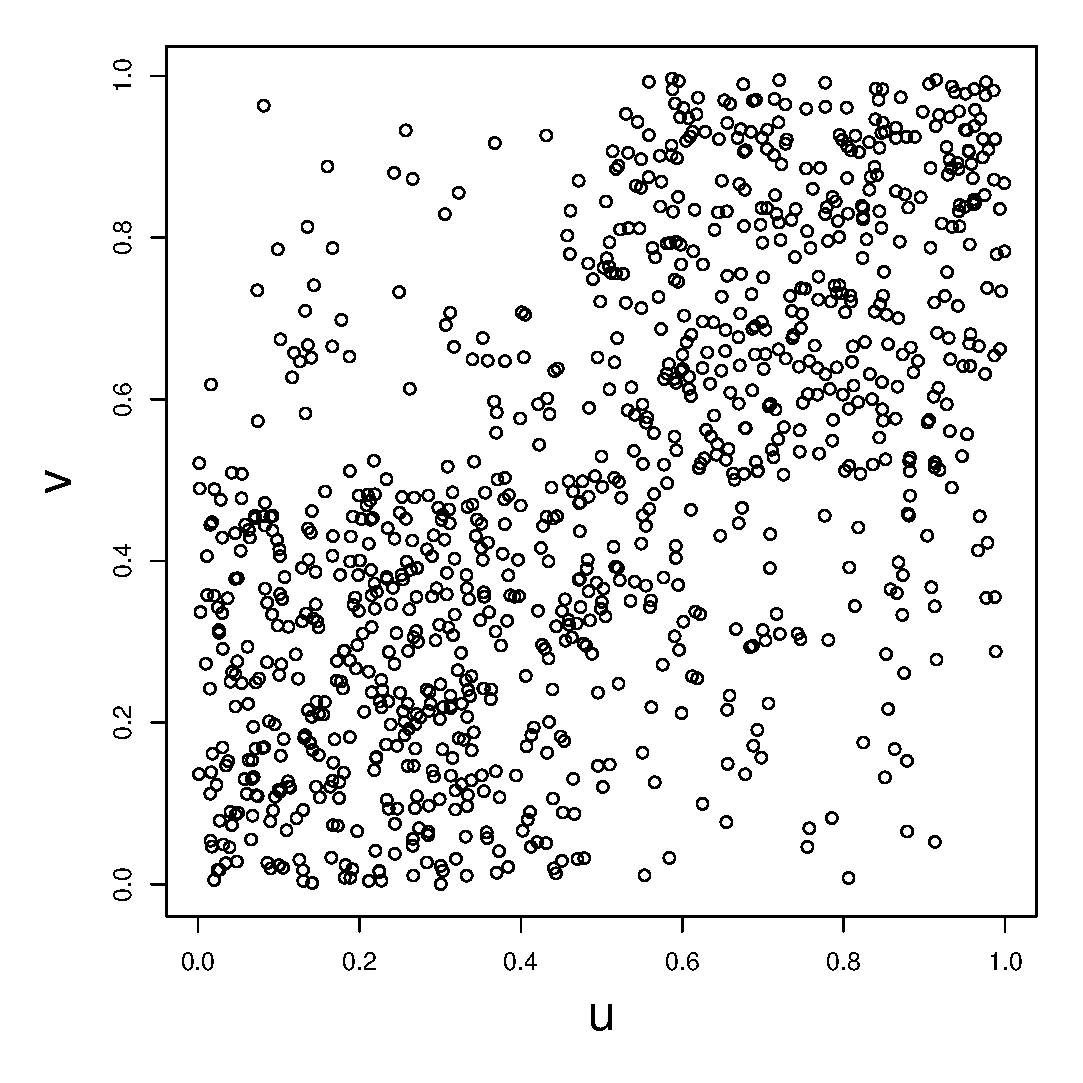
\includegraphics{structural41.eps}} \\
    \end{tabular}
    \caption{Copulas from \fref{fillustration} with equal Spearman's $\rho=0.6$ (black line) and different $\rho_1^*$ (green), $\rho_2^*$ (blue) and $\rho_3^*$ (red).  }
    \label{falternate}
  \end{center}
\end{figure}



\section{Discussion of copula fitting using layer dependence}\label{sfitting}

This section proposes fitting a copula  to data using layer dependence. The approach can  incorporate expert opinion on the dependence structure. The approach is illustrated using historical NASDAQ and FTSE stock returns.

\subsection{Fitting steps}

A copula fitting procedure based on layer dependence is as follows:

\begin{enumerate}
\item Calculate layer dependence curve with desired granularity from percentile rank data.

\item Smooth calculated layer dependence curve either parametrically or semi-parametrically.

\item Refine layer dependence using expert knowledge, such as existence and level of tail dependence, and overall dependence.

\item Fit a copula given the fitted layer dependence curve, for example using the factor copula model described in the next subsection.
\end{enumerate}
The layer dependence approach offers two advantages over fitting parametric copulas. Firstly layer dependence reflects the dependence structure exhibited in past data, whereas parametric copulas, with their relatively restricted dependence structures, may not properly fit past data. Secondly, layer dependence accommodates expert knowledge of local dependence, whereas parametric copulas permit limited changes to the dependence structure once a parametric form is selected.


In comparison to empirical copulas, layer dependence is more robust and less affected by data inadequacies. Layer dependence summarises past data into linear functions of conditional tail means, with a parametric curve fitted to calculated values. Hence layer dependence captures advantages of parametric and empirical copulas -- the fitted copula utilises a smooth layer dependence curve, and the dependence structure underlying the fitted copula mirrors past data.



\begin{comment}

\subsection{Factor copula model}

The following describes an approach to fit and simulate a copula given layer dependence $\ell_\alpha$ for all $0\leq\alpha\leq 1$. The copula is not unique to $\ell_\alpha$ since $\ell_\alpha$, from \eref{gapexp}, relates to first-order conditional expectations rather than the entire conditional distribution associated with the copula.


Suppose $s$ is a random variable. The factor copula model is
\begin{equation}\label{factor}
u=F(s+\eps) \cq
v=F(s+\eta)    \cq \eps, \eta \sim N(0,1) \ ,
\end{equation}
where $s$, $\eps$ and $\eta$ are independent and $F$ is the  distribution of the random variables in the brackets. Then both $u$ and $v$ are uniform and the joint distribution of $(u,v)$ is exchangeable. Exchangeability is assumed since most commonly used copulas, such as Archimedean copulas \citep{mcneil2005qrm}, are exchangeable. The factor copula model in \eref{factor} is made non-exchangeable for example by dropping either $\eps$ or $\eta$.

The common factor $s$ in \eref{factor} generates and controls layer dependence between $u$ and $v$. For example if $s$ is highly volatile and right skewed relative to noise terms $\eps$, $\eta$, then $u$ and $v$ are more dependent particularly in the upper tail. The two panels in \fref{ffactor} simulate factor copulas and their layer dependence curves assuming $s$ has standard normal and $\chi^2_1$ distributions. Standard normal $s$ generates a Gaussian copula, while a $\chi^2_1$ distribution implies movements in $u$ and $v$ close to $1$ are generated and controlled by $s$, implying upper tail dependence.

\begin{figure}
  \begin{center}
    \begin{tabular}{cc}
      \resizebox{60mm}{!}{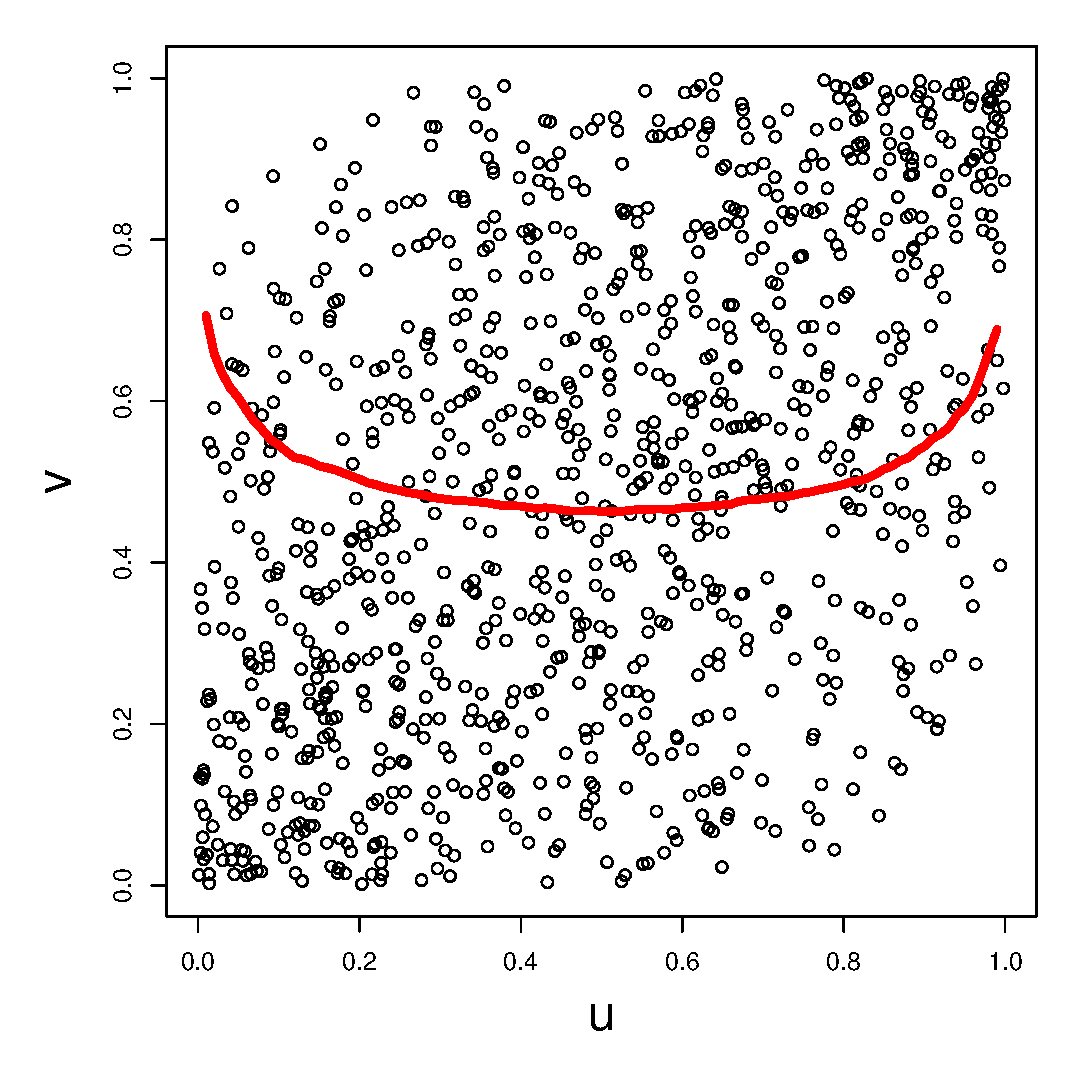
\includegraphics{factor1.eps}}
      \resizebox{60mm}{!}{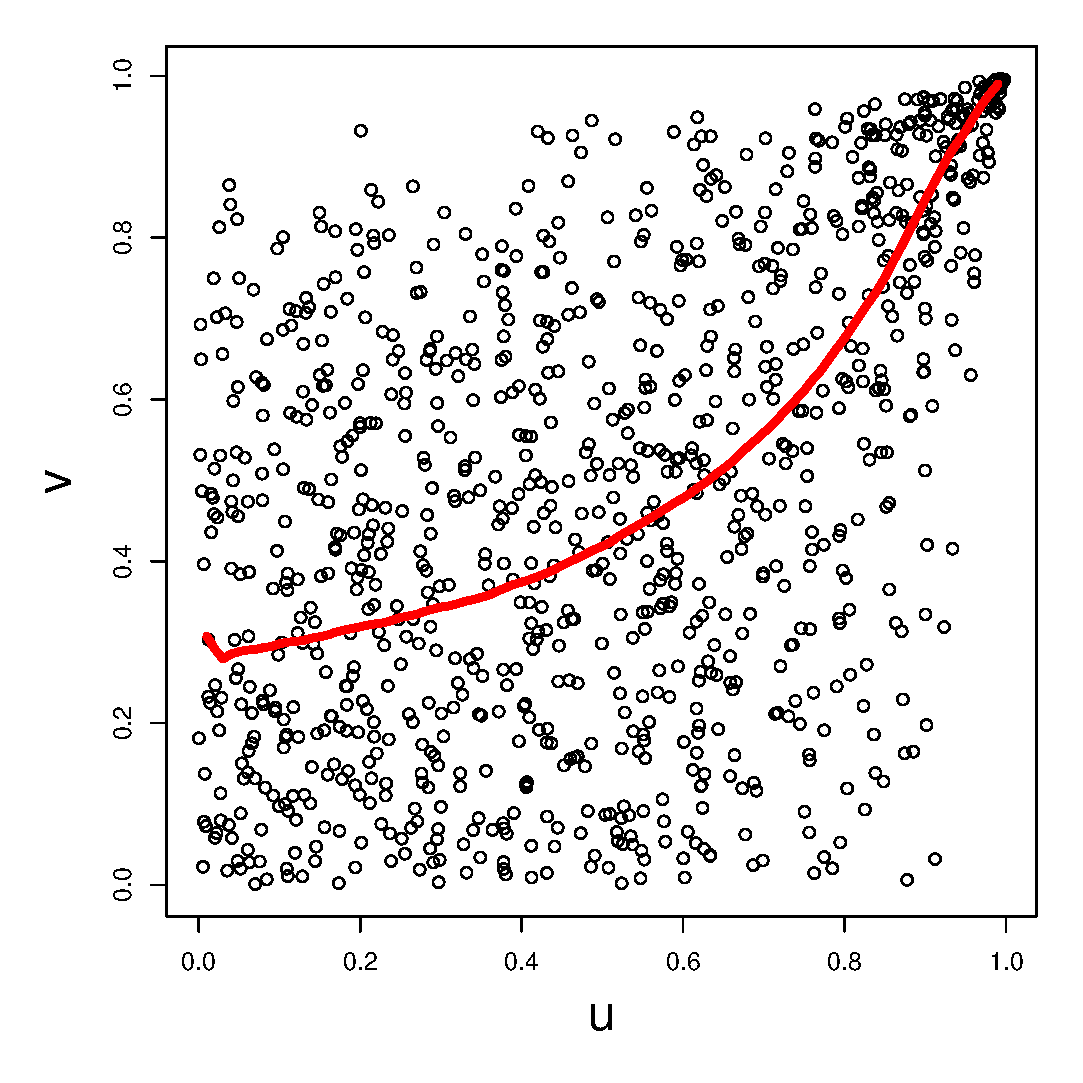
\includegraphics{factor2.eps}} \\
    \end{tabular}
    \caption{Simulated factor copulas and layer dependence curves assuming $s$ is standard normal (left panel) and $\chi^2_1$ (right panel).  }
    \label{ffactor}
  \end{center}
\end{figure}



The factor copula model generates positive layer dependence. Negative layer dependence is created by first simulating the corresponding positive layer dependence, and then taking complements of either percentile rank.

To generate a sample of $(u,v)$ of size $n$ from the factor copula model with layer dependence $\ell_\alpha$, $0\le\alpha\le 1$,  first simulate $\eps_i,\eta_i\sim N(0,1)$ for $i=1,\ldots,n$.  Arbitrarily initialise $s_i$ for $i=1,\ldots,n$ by setting it equal to a normal sample with standard deviation chosen such that $s_i+\eps_{i}$ and $s_i+\eta_{i}$ have Spearman's correlation consistent with $\ell_\alpha$. Then repeat:
\begin{enumerate}

\item Compute ``fitted"  $\hat\ell_{j/n}$ between  $(u_i,v_i)$ for $j=1,\ldots,n$, where $u_i$ and $v_i$ are calculated from the percentile ranks of $s_i+\eps_{i}$ and $s_i+\eta_{i}$, respectively.

\item Keep $s_1$ unchanged and update  $s_2,\ldots,s_n$ according to
$$
s_{i+1}  \leftarrow s_{i}+  \left(\frac{\ell_{i/n}}{\hat \ell_{i/n}}\right)^a(s_{i+1}-s_i)\cq a>0\;,
$$
in turn yielding an updated sample of $(u_i,v_i)$.

\item Go to 1 unless $\|\ell_{i/n} -  \hat\ell_{i/n} \|$ is less than some pre-specified small amount.

\end{enumerate}
Step 1 can be simplified by computing $\hat \ell_{j/n}$ over a fewer number of points and then fitting a parametric curve to computed values. The resulting sample $(u_i,v_i)$ for   $i=1,\ldots,n$ once the iteration is complete has  layer dependence $\hat\ell_\alpha\approx\ell_\alpha$.




\subsection{Illustration using stock returns}

The following illustrates layer dependence copula fitting using NASDAQ and FTSE returns. The top left panel in \fref{fmarketindex} plots percentile ranks of daily NASDAQ and FTSE returns from $1985$ and $2014$. Layer dependence  at every integer percentile and Spearman's correlation are shown in the same panel. Spearman's correlation is $0.4$, indicating moderate dependence between NASDAQ and FTSE returns. Layer dependence increases towards both tails, but more so in the lower tail. Hence major corrections in NASDAQ and FTSE tend to occur simultaneously, and negative corrections are more strongly dependent than positive corrections.

The top right panel in \fref{fmarketindex} fits a factor copula to a smooth layer dependence curve passing through empirical values\footnote{The smoothing is performed by fitting a polynomial of order 4 using least squares estimation.}. Simulated values of the fitted factor copula are shown in the same panel. The bottom left panel fits a Gaussian copula to past data by matching Spearman's correlation. The Gaussian copula has a symmetric layer dependence curve, and hence does not capture the stronger lower tail dependence exhibited in NASDAQ and FTSE data.  Student-$t$ and other elliptical copulas would suffer from the same inadequacy.

The bottom right panel in \fref{fmarketindex} plots the density of the common factor $s$ generating the fitted factor copula. Also shown is the density implicit in the fitted Gaussian copula. The density of $s$ is more peaked and left skewed, reflecting the stronger lower tail dependence and weak dependence in the centre.


\begin{figure}
  \begin{center}
    \begin{tabular}{cc}
      \resizebox{60mm}{!}{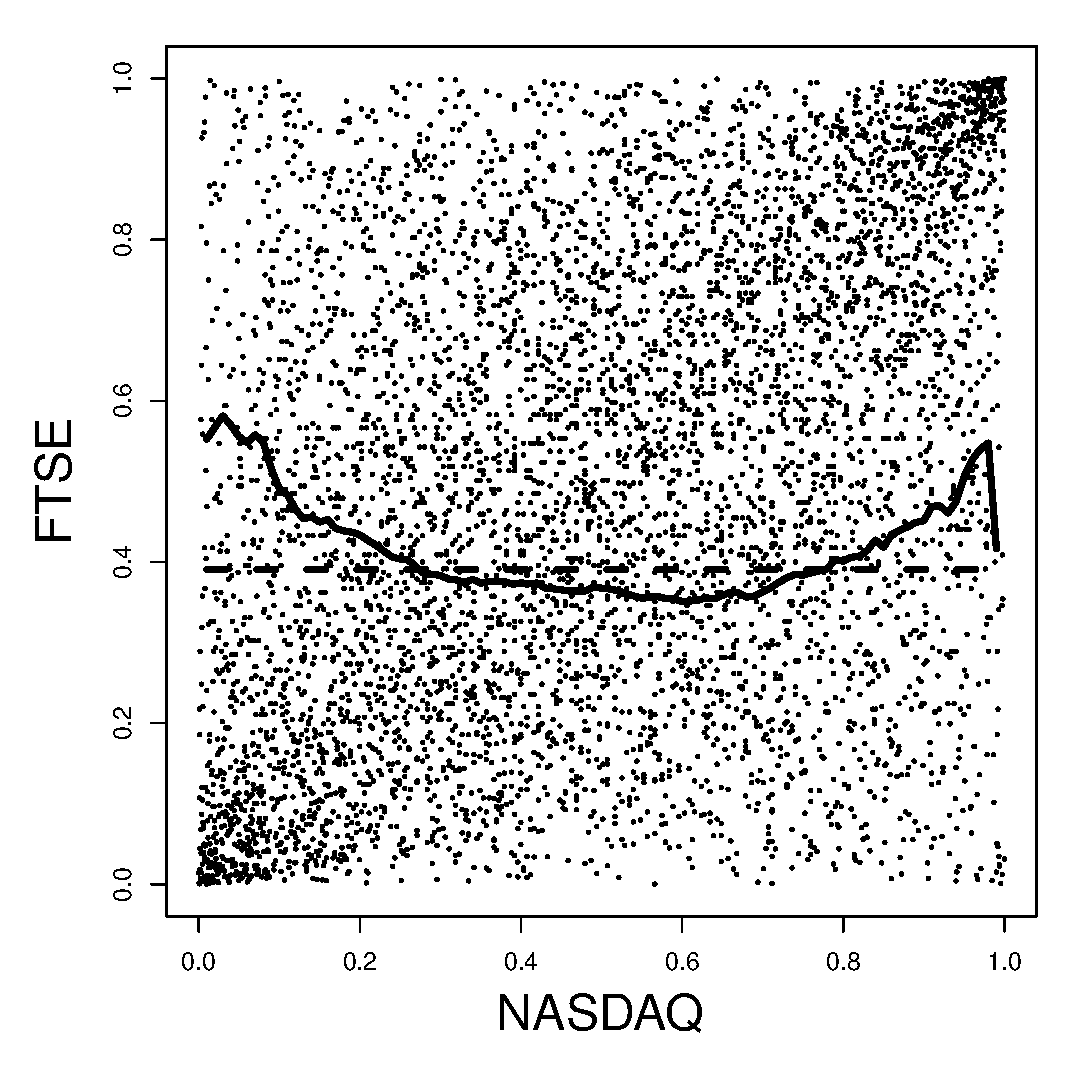
\includegraphics{NASDAQvsFTSE.eps}}
      \resizebox{60mm}{!}{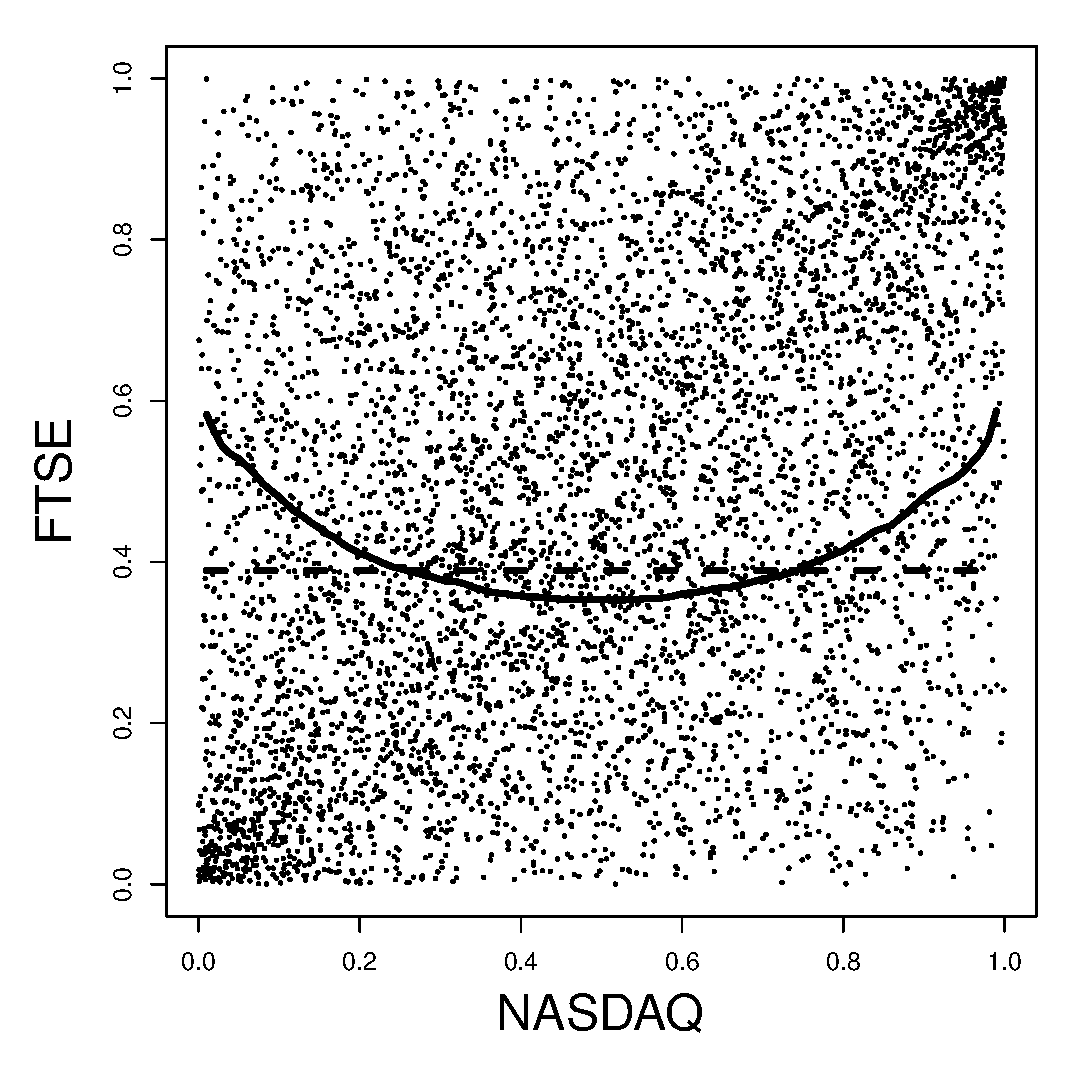
\includegraphics{NASDAQvsFTSE_fitted.eps}} \\
      \resizebox{60mm}{!}{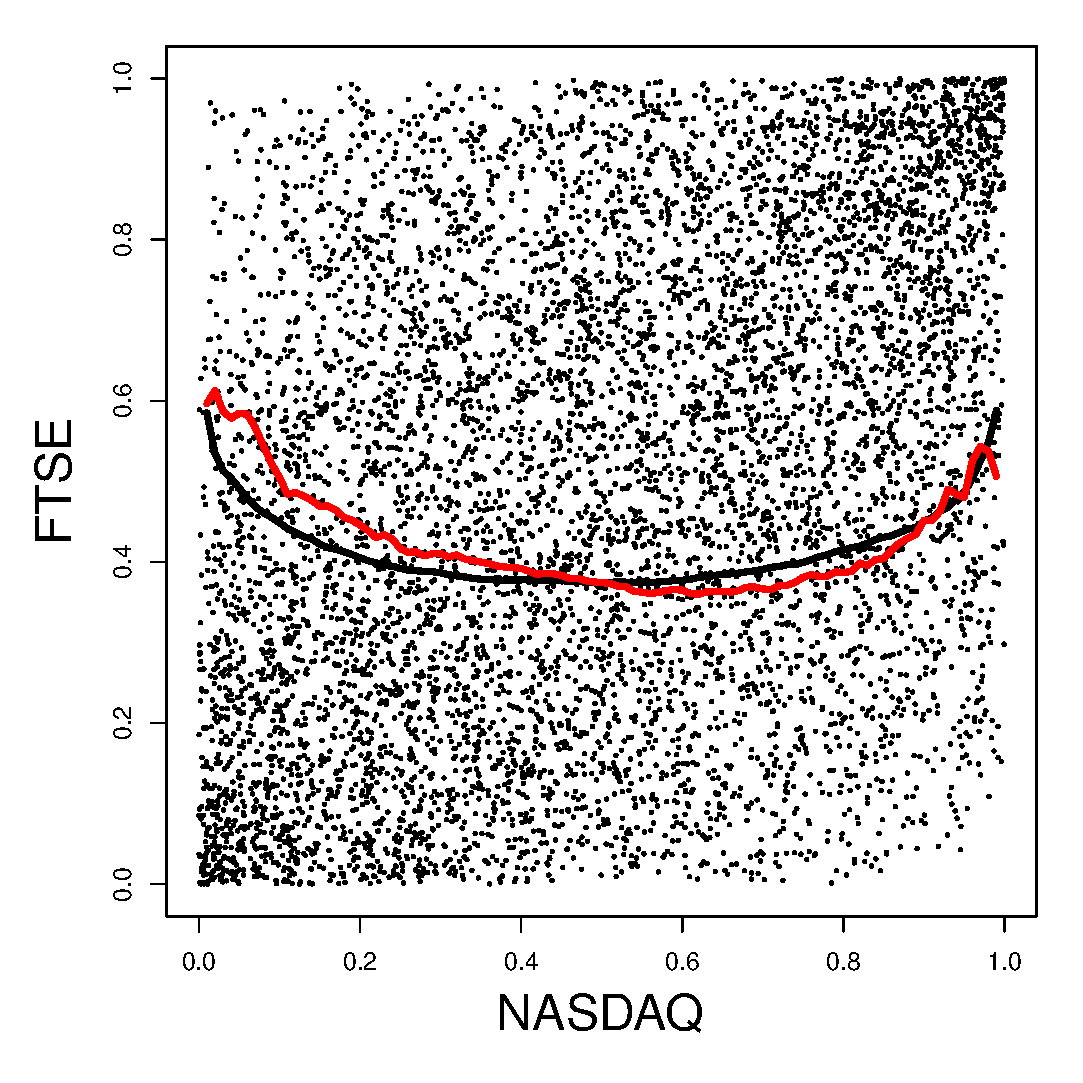
\includegraphics{gaussianfitted.eps}}
      \resizebox{60mm}{!}{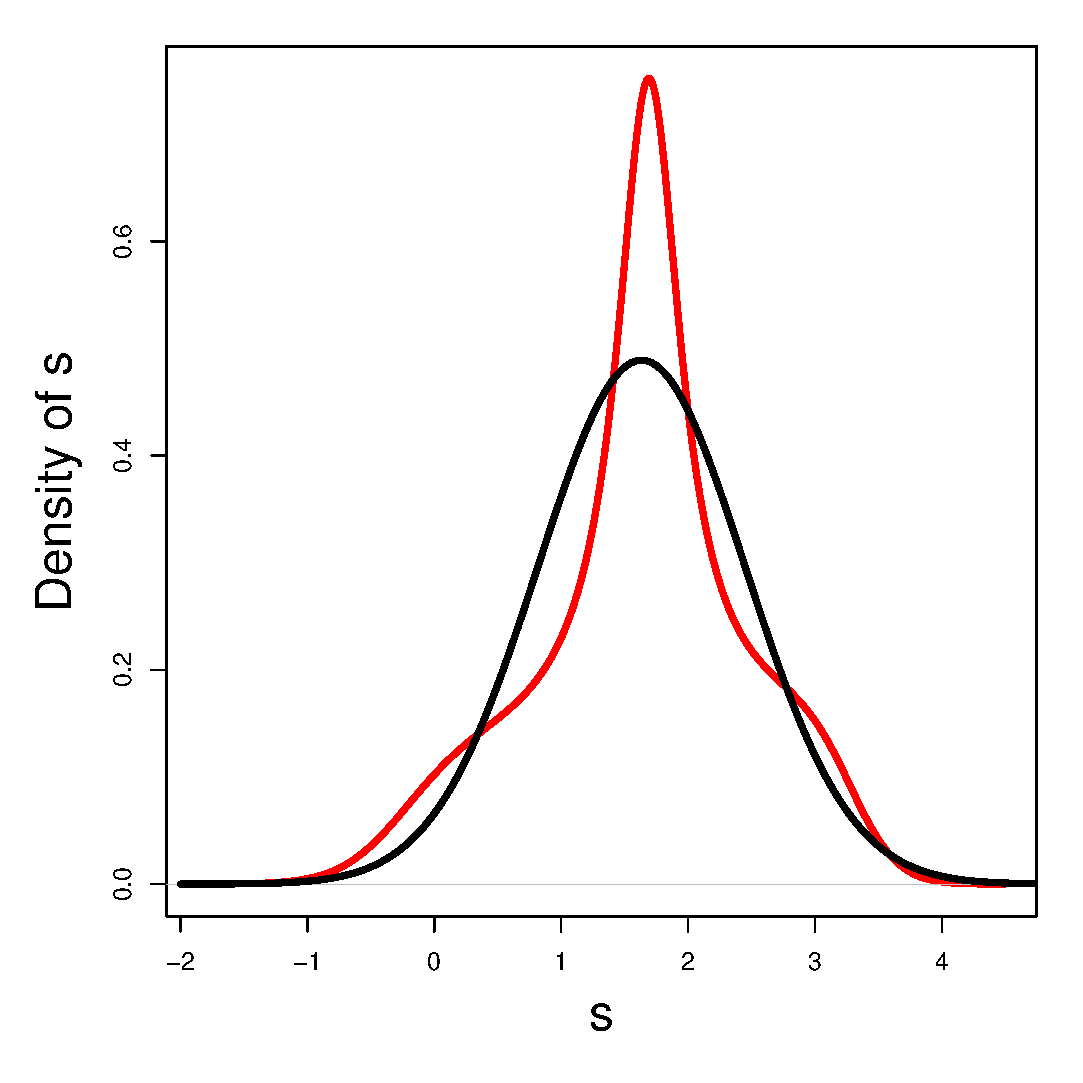
\includegraphics{densities.eps}} \\
    \end{tabular}
    \caption{The top left panel plots percentile ranks of NASDAQ and FTSE daily returns from 1985 to 2014, and the empirical layer dependence curve. The top right panel plots a parametrically smoothed layer dependence curve and a fitted factor copula. The bottom left panel plots a Gaussian copula and its layer dependence curve. The Gaussian copula is fitted by matching Spearman's correlation. The red empirical layer dependence curve is plotted in both panels containing fitted factor and Gaussian copulas. The bottom right panel graphs the density of $s$ underlying the fitted factor copula (red), and the implied density of $s$ underlying the Gaussian copula (black).}
    \label{fmarketindex}
  \end{center}
\end{figure}



\end{comment}


\begin{comment}
\subsection{Regression model}

The second approach exploits the relation $\tau_\alpha=(1+\alpha\ell_\alpha)/2$ where $\tau_\alpha$ is the upper conditional tail expectation $\E(v|u>\alpha)$.  Then
$$
\tau'_\alpha \equiv\frac{\de\E(v|u>\alpha)}{\de\alpha}= \frac{\de}{\de \alpha} \frac{\E\left\{v(u>\alpha)\right\}}{1-\alpha}
= \frac{\tau_\alpha-\mu_\alpha}{1-\alpha}\cq \mu_\alpha\equiv \E(v|u=\alpha)\;,
$$
where $\mu_\alpha$ is the regression curve of $v$ on $u$. Hence $\mu_\alpha=\tau_\alpha-(1-\alpha)\tau'_\alpha$
and $\tau_\alpha$ is monotonic if $\mu_\alpha$ is monotonic.

Suppose $\ell_\alpha$ and hence $\tau_\alpha$ is given for $\alpha=i/n$, $i=1,\ldots,n$ with values denoted $\tau_1,\tau_1,\ldots,\tau_{n}$.   Then  $C(u,v)$ with layer dependence $\ell_\alpha$ is simulated using
$$
v_i=F\{F^-(\mu_i)+\sigma\eps_i\}\ ,\ \mu_{i}=\tau_i - (n-i)(\tau_{i}-\tau_{i-1})\ ,\ \eps_i\sim N(0,1)\ ,\  i=1,\ldots,n\ ,
$$
with $\tau_0=1/2$ and $\sigma$ chosen so that Spearman's $\rho$ for the each sample is expected to match $\rho_S$ implied by $\ell_\alpha$ as in \eref{wtdaverage}.  Here $F$ is an appropriate distribution such as the normal or  logit:  $F^-(\mu_i)=\ln\{\mu_i/(1-\mu_i)\}$.  In the logic case setting $\sigma=1$ appears to ensure a match between the theoretical and empirical $\rho_S$.  To enforce the $v_1,\ldots,v_n$ are empirically uniform the final $F$ transformation $F$ is replaced by computing  empirical percentiles.
\end{comment}


\begin{comment}

\subsection{Measuring dependence asymmetry}

Dependence asymmetry is the difference between dependence in the upper tail compared to lower tail. Dependence asymmetry is important for example when modeling the sum of two random variables. Strong upper tail dependence relative to lower tail increases the right skewness of the sum since large outcome of both random variables are more likely to occur simultaneously.

Measure dependence asymmetry as $\ell^+-\ell^-$ where
$$
 \ell^+ \equiv \int_z^1 w_\alpha\ell_\alpha \de \alpha
\cq \ell^- = \int_0^{1-z} w_\alpha\ell_\alpha \de \alpha
\cq 0.5\leq z\leq 1\;,
$$
and $w_\alpha$ is a weighting function symmetric about $\alpha=0.5$. Hence dependence in the upper tail is the weighted average of layer dependence over percentiles above $z$, and dependence in the lower tail averages over percentiles below $1-z$ using identical weights. For example the Gaussian or $t$ copulas with symmetric dependence have $\ell^+-\ell^-=0$. For the Clayton copula, $\ell^+-\ell^-<0$ while $\ell^+-\ell^->0$ for the Gumbel copula.

Substituting the expression for $\ell_\alpha$ in \eref{definition} yields
$$
\ell^+
= \cov\left\{ v, \int_z^1 \frac{(u>\alpha)}{0.5\alpha(1-\alpha)} w_\alpha \de \alpha\right\}
=\cov\left\{v,(u>z)\int_z^u \frac{2w_\alpha}{\alpha(1-\alpha)} \de \alpha\right\}
$$
and similarly
$$
\ell^- =  \cov\left\{ v, \int_0^{1-z} \frac{(u>\alpha)}{0.5\alpha(1-\alpha)} w_\alpha \de \alpha\right\}
=\cov\left\{ v, (u\leq 1-z) \int_0^u \frac{2w_\alpha}{\alpha(1-\alpha)} \de \alpha \right\}
$$
$$
+\cov\left\{ v, (u> 1-z)  \right\} \int_0^{1-z}\frac{2w_\alpha}{\alpha(1-\alpha)} \de \alpha \;.
$$
\end{comment}

\begin{comment}

\section{Layer dependence between non--uniform random variables}\label{soriginal}


Consider random variables $x$ and $y$.  Analogous to \eref{definition}, define layer dependence between $x$ and $y$ as the scaled covariance between $y$ and $k$--layer of $x$:
$$
\ell_k^* \equiv \frac{\cov\{y,(x>k)\}}{\cov\{y^*,(x>k)\}} = \frac{\cor\{y,(x>k)\}}{\cor\{y^*,(x>k)\}}\;,
$$
where $k$ lies in the support of $x$, and $y^*$ has identical marginal distribution as $y$ and is comonotonic with $x$. The denominator hence ensures $\ell_k^*=1$ for all $k$ when $x$ and $y$ are comonotonic.

Layer dependence $\ell_k^*$ partially satisfies coherence properties of $\ell_\alpha$ in section \aref{scoherence}. If $x$ and $y$ are independent or comonotonic then $\ell_k^*=0$ and $1$, respectively, for all $k$. If $x$ and $y$ are countermonotonic then write $x=F^-(u)$ and $y=G^-(1-u)$ where $F^-$ and $G^-$ are inverse distribution functions of $x$ and $y$, respectively. Layer dependence in this case is
$$
\ell_k^*  =\frac{\cov\{G^-(1-u),(u>\alpha)\}}{\cov\{G^-(u),(u>\alpha)\}} \leq 0 \cq \alpha=F(k) \;,
$$
reducing to $-1$ if $G^-$ is symmetric: $G^-(1-u)-G(0.5)=G(0.5)-G(u)$. Layer dependence $\ell_k^*$ also preserves correlation order: if $x$ and $y$ increase in correlation order in the sense of \cite{dhaene2009correlation} then $\ell_k^*$ is higher for all $k$, since higher correlation order translates to higher covariance values. Layer dependence $\ell_k^*$ is symmetric if the distribution of $y$ is symmetric.

Averaging $\ell_k^*$ yields a link to correlation between $x$ and $y$:
$$
\int \frac{\cov\{y^*,(x>k)\}}{\cov(y^*,x)} \ell^*_k \de k =  \frac{\int \cov\{y,(x>k)\} \de k}{\cov(y^*,x)}
= \frac{\cov(x,y)}{\cov(x,y^*)} = \frac{\cor(x,y)}{\cor(x,y^*)}
$$
applying the result in \eref{decompose}.

The four panels \fref{foriginalscale} calculate layer dependence curves between $x$ and $y$ with combinations of symmetric and right skewed beta marginal distributions. A Gumbel copula is assumed. Layer dependence between percentile ranks is included for comparison. Layer dependence retains its overall shape when observed random variables are used instead of percentile ranks.

\begin{figure}
  \begin{center}
    \begin{tabular}{cc}
      \resizebox{60mm}{!}{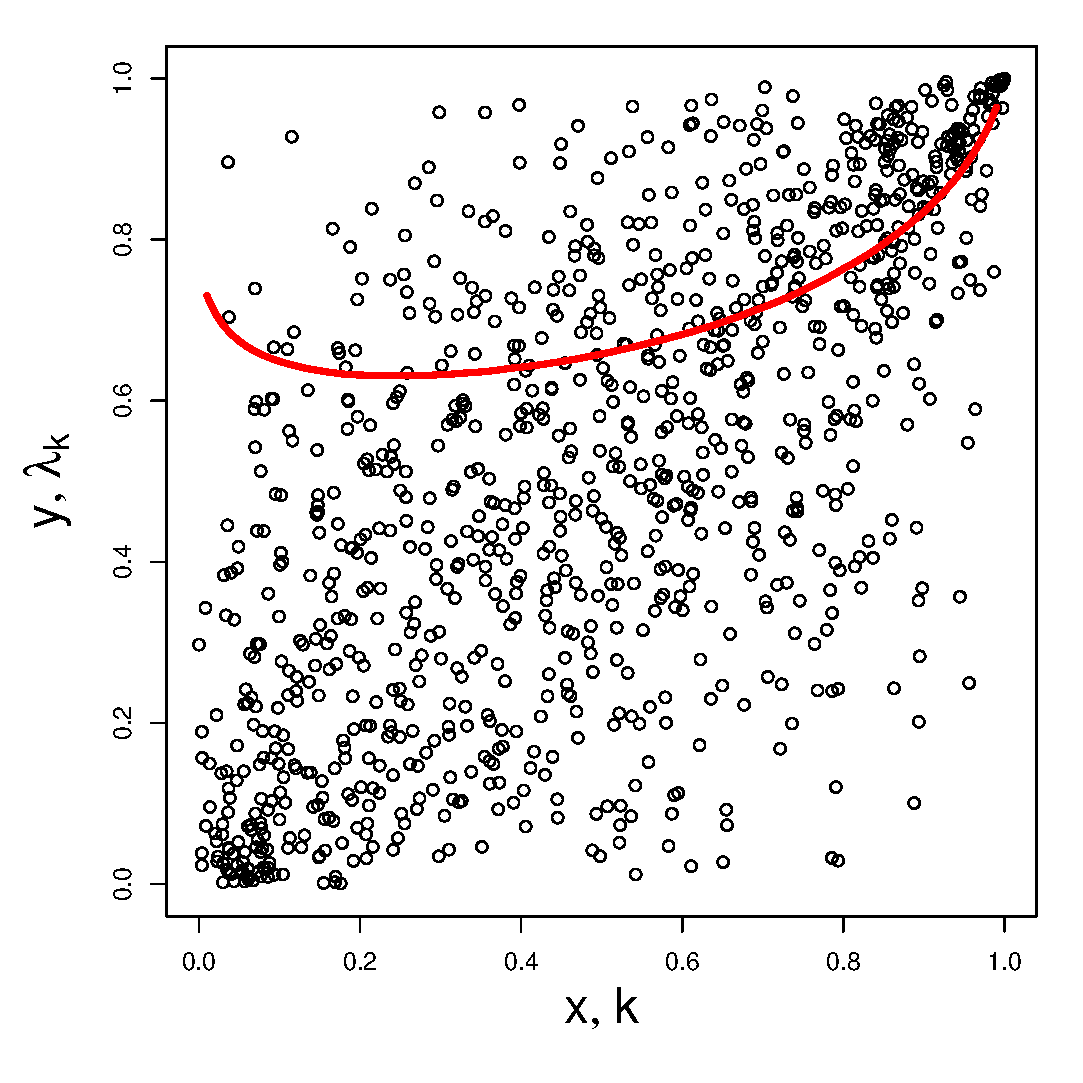
\includegraphics{gumbel0.eps}}
      \resizebox{60mm}{!}{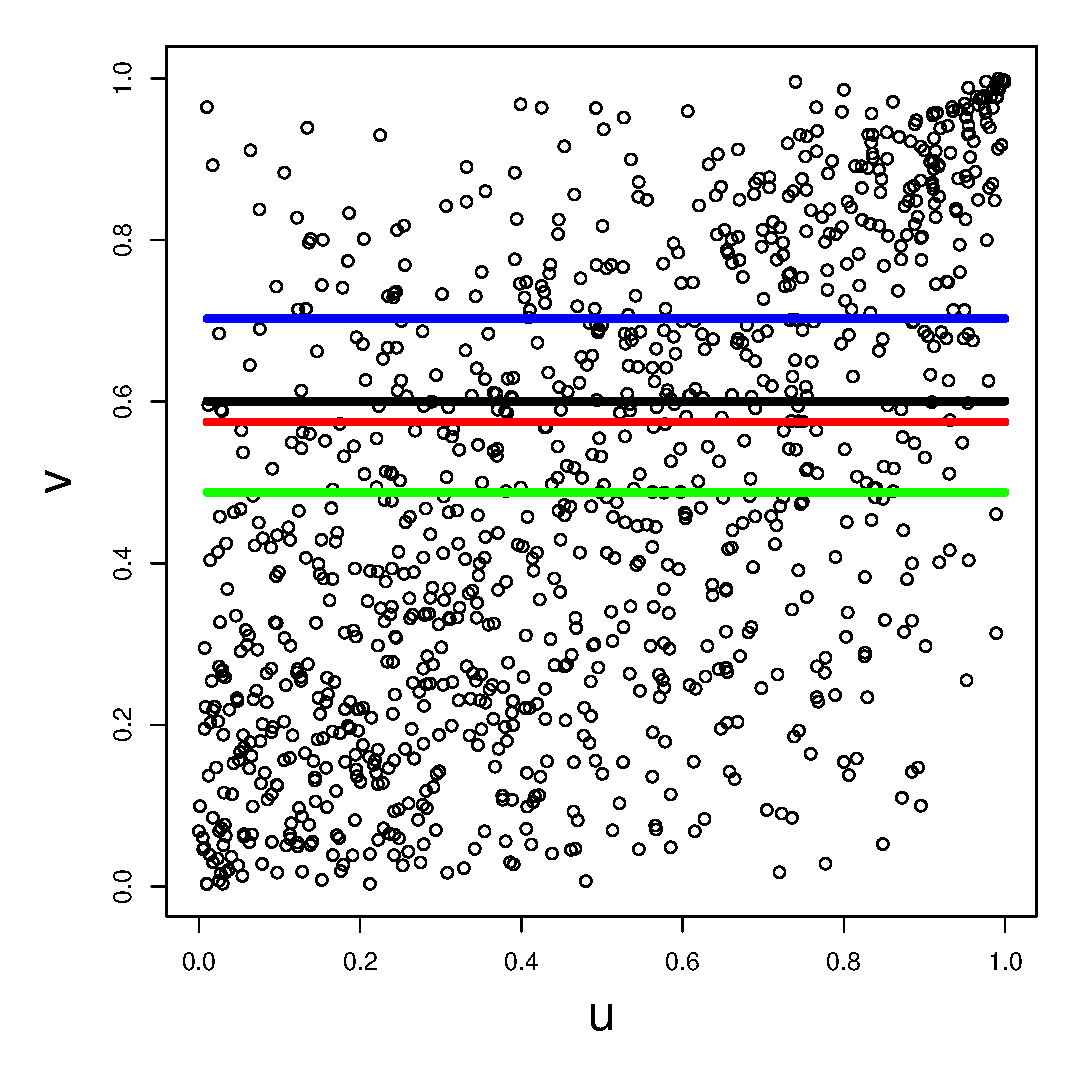
\includegraphics{gumbel1.eps}} \\
      \resizebox{60mm}{!}{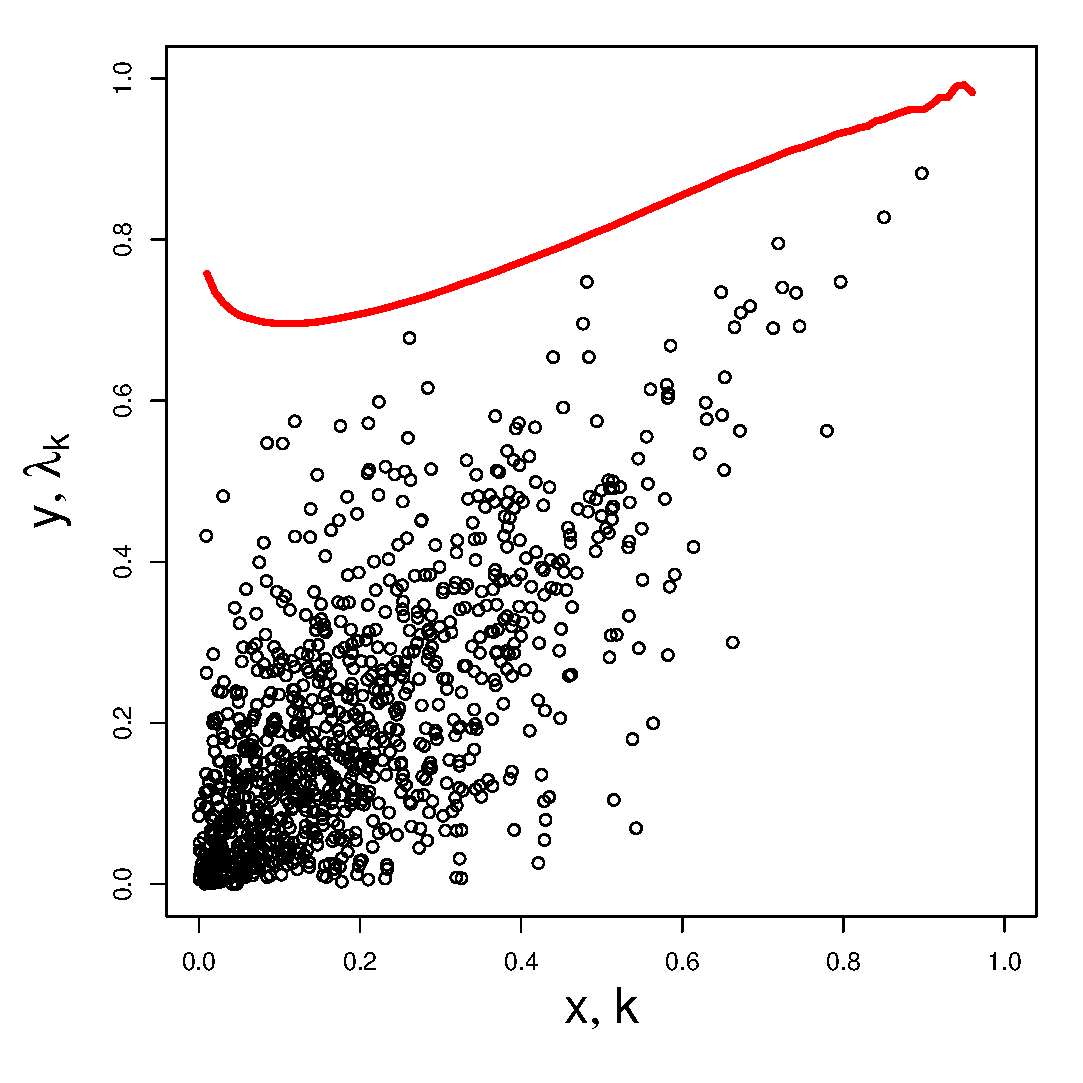
\includegraphics{gumbel2.eps}}
      \resizebox{60mm}{!}{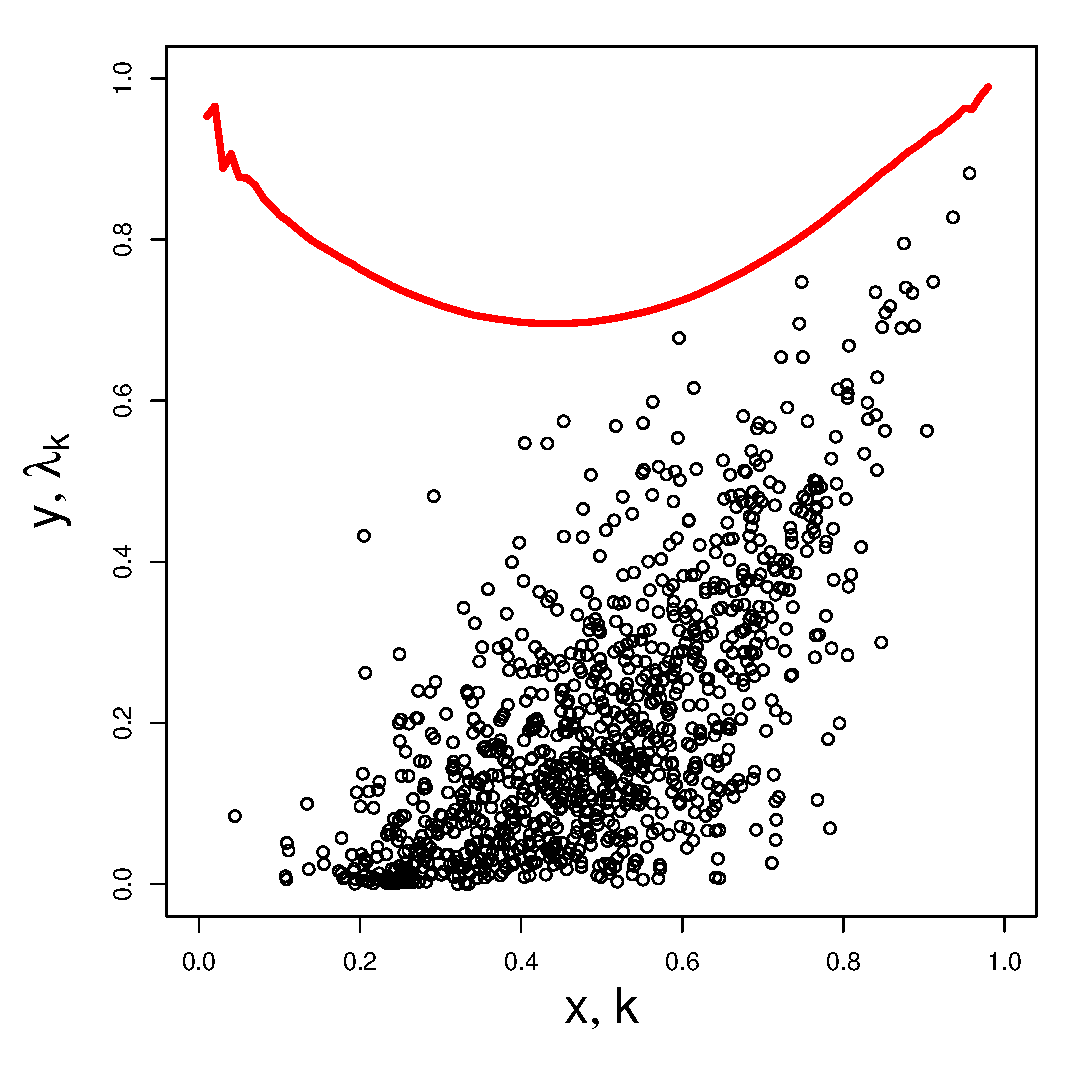
\includegraphics{gumbel3.eps}} \\
    \end{tabular}
    \caption{Layer dependence curves between $x$ and $y$ (red line) for a Gumbel copula. The top left panel assumes uniform $x$ and $y$, yielding original layer dependence. The top right panel assumes symmetric $x$ and $y$. The bottom left panel assumes right skewed $x$ and $y$. The bottom right panel assumes symmetric $x$ and right skewed $y$.}
    \label{foriginalscale}
  \end{center}
\end{figure}

\end{comment}


\begin{comment}
\subsection{Gap between conditional tail expectations}

Manipulating layer dependence $\ell_\alpha^*$ yields
$$
\ell_\alpha^* = \frac{\E(y|x>V_\alpha)-\E(y|x\leq V_\alpha)}{\E(y^*|x>V_\alpha)-\E(y^*|x\leq V_\alpha)}
=\frac{\E(y|u>\alpha)-\E(y|u\leq\alpha)}{\E(y^*|u>\alpha)-\E(y^*|u\leq\alpha)} \;,
$$
the gap between upper and lower conditional tail expectations of $y$. A similar expression for original layer dependence $\ell_\alpha$ exists in \eref{gapexp}, where conditional tail expectations of percentile rank $v$ are evaluated instead of $y$.

Using the income-education example in \sref{sintroduction}, the population is again divided into two segments depending on whether education is below or above the $\alpha$-percentile. Average actual income is measured in each segment rather than average income ranking. The calculated gap in average actual income is divided by the maximum gap, or the difference between average actual income above and below the $\alpha$-percentile.


\subsection{Link to Pearson correlation}

Taking the following weighted average of $\ell_\alpha^*$ yields scaled Pearson correlation between $x$ and $y$:
$$
\int_0^1 \ell_\alpha^* \left[\frac{\cov\{y^*,(u>\alpha)\}V_\alpha'}{\cov(y^*,x)} \right] \de \alpha
= \frac{\cov\left\{y, \int_0^1 (u>\alpha)V_\alpha' \de \alpha \right\}}{\cov(y^*,x)} =\frac{\cov(y,V_u)}{\cov(y^*,x)}
$$
$$
= \frac{\cor(y,x)}{\cor(y^*,x)}
\cq \int_0^1 \frac{\cov\{y^*,(u>\alpha)\}V_\alpha'}{\cov(y^*,x)}  \de \alpha= \frac{\cov(y^*,V_u)}{\cov(y^*,x)} = 1 \;,
$$
where weights integrate to one. The denominator $\cor(y^*,x)$ in scaled Pearson correlation ensures unity if $x$ and $y$ are comonotonic. Similarly a weighted average of layer dependence $\ell_\alpha$ over all $\alpha$, using quadratic weights, yields  $\rho_S$ as shown in \eref{wtdaverage}.

\subsection{Relationship between two layer dependences}

layer dependences between original random variables and between their percentile ranks are generated by a common ``dependence generating function"
$$
g_{\alpha,\beta}\equiv \frac{\cov\{(u>\alpha,v>\beta)\}}{\cov\{(u>\alpha,u>\beta)\}}
= \frac{C(\alpha,\beta)-\alpha\beta}{\min(\alpha,\beta)-\alpha\beta}  \cq 0\leq \alpha,\beta\leq 1\;,
$$
where $C$ is the copula underlying $(u,v)$. The dependence generating function $g_{\alpha,\beta}$ measures dependence between $\alpha$-layer of $x$ and $\beta$-layer of $v$. In particular $g_{\alpha,\beta}=1$ for all $\alpha$ and $\beta$ if $u$ and $v$ are perfectly dependent, and $g_{\alpha,\beta}=0$ if $u$ and $v$ are independent. Negative dependence yields negative $g_{\alpha,\beta}$.

Taking a weighted average of $g_{\alpha,\beta}$ over all $\beta$ yields layer dependence, between percentile ranks and between observed random variables. Layer dependence $\ell_\alpha$ is generated by the weighted integral
$$
\ell_\alpha= \int_0^1 w_{\beta,1} g_{\alpha,\beta} \de\beta
\cq w_{\beta,1}=\frac{\min(\alpha,\beta)-\alpha\beta}{\int_0^1 \{\min(\alpha,\beta)-\alpha\beta\}\de\beta}
=\frac{\min(\alpha,\beta)-\alpha\beta}{0.5\alpha(1-\alpha)}
$$
and layer dependence $\ell_\alpha^*$ is generated by a different weighted integral
$$
\ell_\alpha^* = \int_0^1 w_{\beta,2}   g_{\alpha,\beta} \de G^-(\beta)
\cq w_{\beta,2}=\frac{\min(\alpha,\beta)-\alpha\beta}{\int_0^1 \{ \min(\alpha,\beta)-\alpha\beta\}\de G^-(\beta)}
$$
$$
=\frac{\min(\alpha,\beta)-\alpha\beta}{\cov \{G^-(u),(u>\alpha)\}}  \;.
$$
For $\ell_\alpha^*$, weights attached to $g_{\alpha,\beta}$ are proportional to the derivative $(G^-)'$. Hence $g_{\alpha,\beta}$ is weighted more heavily over values of $\beta$ where the derivative $\{G^-(\beta)\}'$ is large, such as in the tail of a right skewed distribution. In comparison weights for layer dependence $\ell_\alpha$ are ``marginal free."

The dependence generating function captures complete dependence information due to its direct relationship with the copula $C$. Correlations $\cor(u,v)$ and $\cor(x,y)$ show completely summarised dependence information. Layer dependences $\ell_\alpha$ and $\ell_\alpha^*$ balances the extremes and shows dependence information on a single dimension.

\end{comment}



\begin{comment}

\section{Comparison with existing local dependence measures}\label{sliterature}

This section compares layer dependence with existing local dependence measures: tail concentration \citep{venter2002tails}, correlation curve \citep{bjerve1993correlation}, and bivariate measures by \cite{bairamov2003new}, \cite{jones1996local} and \cite{holland1987dependence}. Calculations are applied to copulas in \fref{fillustration}. Layer dependence is more reflective of local dependence (dispersion and concordance between points), and satisfies all five coherence properties in \sref{scoherence}. In addition there is a direct relationship between layer dependence and  $\rho_S$ in \eref{wtdaverage}.



\subsection{Tail concentration}

\cite{venter2002tails} defines tail concentration at $0\leq\alpha\leq 1$ by combining lower and upper conditional tail probabilities relative to $\alpha$:
\begin{equation}\label{tailcon}
\tau_\alpha \equiv (\alpha\leq 0.5) \p(v\leq \alpha|u\leq \alpha) + (\alpha>0.5)\p(v>\alpha|u>\alpha) \;.
\end{equation}
Higher tail concentration implies $u$ and $v$ are more likely to fall in the same lower tail ($\alpha\leq 0.5$) or upper tail ($\alpha>0.5$). Tail concentration partially satisfies coherence properties described in \sref{scoherence}, and partially reflects local dependence. Layer dependence refines tail concentration through standardisation and reflecting average dispersion between discordant points. Further discussion of tail concentration is shown below.

Rewrite tail concentration in terms of the copula $C$ of $(u,v)$:
$$
\tau_\alpha = (\alpha\leq 0.5)\frac{C(\alpha,\alpha)}{\alpha}+(\alpha>0.5)\frac{1-2\alpha+C(\alpha,\alpha)}{1-\alpha} \;,
$$
therefore tail concentration depends only on the diagonal section of the copula, and is hence symmetric in $u$ and $v$. Independence implies $\tau_\alpha=\alpha(\alpha\leq 0.5)+(1-\alpha)(\alpha>0.5)$, and comonotonicity and countermonotonicity yield $\tau_\alpha=1$ and $\tau_\alpha=0$, respectively. Hence tail concentration does not satisfy independence and perfect dependence (countermonotonicity) coherence properties. Symmetry is also not satisfied since tail concentration is non-negative. The ordering property is satisfied since tail concentration increases with the copula $C$. Lastly $0\leq\tau_\alpha\leq 1$ since $\tau_\alpha$ is a probability, hence the bounds property holds.

Standardising tail concentration improves its coherence and reflection of local dependence. The latter is demonstrated via an illustration below. Standardisation involves subtracting the value assuming independence, and dividing the result by its maximum value:
$$
\tau_\alpha^* \equiv \frac{\tau_\alpha - \{\alpha(\alpha\leq 0.5)+(1-\alpha)(\alpha>0.5)\}}{1-\{\alpha(\alpha\leq 0.5)+(1-\alpha)(\alpha>0.5)\}}
=\frac{C(\alpha,\alpha)-\alpha^2}{\alpha(1-\alpha)} = \gamma_\alpha \;.
$$
Standardised tail concentration $\tau_\alpha^*=0$ if $u$ and $v$ (independence property), and is negative if $u$ and $v$ are negatively dependent. Standardised tail concentration is also equal to the measure of concordance $\gamma_\alpha$ defined in \eref{concordance}.

From \eref{decomposition}, layer dependence combines standardised tail concentration $\tau_\alpha^*=\gamma_\alpha$ and average dispersion between discordant points $\delta_\alpha$. Hence layer dependence refines tail concentration in two ways:
\begin{itemize}

\item layer dependence includes standardisation to achieve coherence. Standardisation also yields a more accurate reflection of local dependence.

\item layer dependence reflects average dispersion between discordant $u$ and $v$, yielding additional accuracy in local dependence measurement.
\end{itemize}
\fref{fventerillustration} demonstrates the above refinements by comparing tail concentration, its standardised value and layer dependence using identical copulas as \fref{fillustration}. Tail concentration, without standardisation, does not always trace local dependence. For example tail concentration decreases at the upper tail of the Gumbel copula, despite upper tail dependence. Similarly for the Clayton copula. Standardisation corrects these inconsistencies. Layer dependence further refines the calculation by reflecting dispersion between discordant points. For example layer dependence increases to one at the upper tail of the Gumbel copula and lower tail of the Clayton copula, whereas standardised tail concentration does not increase completely to one, despite the presence of tail dependence. In addition standardised tail concentration decreases significantly at both tails of Guassian and Frank copulas although there is no increased dispersion of $(u,v)$ in those areas.
\begin{figure}
  \begin{center}
    \begin{tabular}{cc}
      \resizebox{60mm}{!}{\includegraphics{vnormal.eps}}
      \resizebox{60mm}{!}{\includegraphics{vgumbel.eps}} \\
      \resizebox{60mm}{!}{\includegraphics{vclayton.eps}}
      \resizebox{60mm}{!}{\includegraphics{vfrank.eps}} \\
    \end{tabular}
    \caption{Calculation of tail concentration (blue line) for a Gaussian copula (top left), Gumbel copula (top right), Clayton copula (bottom left) and Frank copula (bottom right). Standardised values (dotted line) and layer dependence (red line) are also shown in each panel.}
    \label{fventerillustration}
  \end{center}
\end{figure}



\subsection{Correlation curve}

\cite{bjerve1993correlation} defines correlation curve based on the conditional distribution of $v$ given $u$. Correlation curve has similar values and coherence properties as layer dependence. However calculated values of correlation curve are volatile due to reliance on a ``pointwise" conditional distribution.

From \cite{bjerve1993correlation}, the correlation curve of $v$ with respect to $u$ at $\alpha$ is defined as
$$
c_\alpha \equiv \frac{\sigma\mu_\alpha'}{\sqrt{(\sigma\mu_\alpha')^2+\sigma_\alpha^2}} = \sign(\mu_\alpha') \times \frac{1}{\sqrt{1+s_\alpha^2}}
\cq 0\leq\alpha\leq 1 \;,
$$
$$
s_\alpha^2\equiv \left(\frac{\sigma_\alpha}{\mu_\alpha'\sigma}\right)^2  \cq \sigma^2\equiv \var(v) \cq \sigma_\alpha^2\equiv \var(v|u=\alpha)
\cq \mu_\alpha\equiv \E(v|u=\alpha) \;.
$$
where $\mu_\alpha$ and $\sigma_\alpha^2$ are the conditional mean and variance of $v$ at $u=\alpha$, respectively, and $\sigma^2=1/12$ is the unconditional variance of $v$. In addition $\mu_\alpha'$ is the derivative of $\mu_\alpha$ with respect $\alpha$. \cite{bjerve1993correlation} also generalises the correlation curve by replacing mean and variance with other location and scale measures such as median and interquartile range, respectively.


The correlation curve $c_\alpha$ at any $\alpha$ is affected by two factors: the derivative $\mu'_\alpha$ and the ratio $\sigma_\alpha^2/\sigma^2$. The former is the sensitivity of the conditional mean of $v$ to changes in $u=\alpha$. Higher sensitivity implies stronger local dependence between $u$ and $v$, increasing $c_\alpha$. The second is the conditional variance of $v$ relative to the unconditional variance. A higher ratio implies values of $v$ conditional on $u=\alpha$ are more variable, hence the conditional mean of $v$ at $u=\alpha$ is a less satisfactory predictor of $v$. The result is lower local dependence and $c_\alpha$.


Correlation curve satisfies similar coherence properties as layer dependence. In particular, for all $\alpha$, $-1\leq c_\alpha\leq 1$ and $c_\alpha=-1$, $0$ and $1$ if $u$ and $v$ are countermonotonic, independent and comonotonic, respectively. Replacing $u$ or $v$ with its complement reverse the sign of $c_\alpha$. In addition $c_\alpha$ increases when $u$ and $v$ are more ``regression dependent.'' \cite{bjerve1993correlation} further discusses properties of correlation curves.


\fref{fcorcurve} graphs correlation curves using identical copulas as \fref{fillustration}. Layer dependence is included as a comparison. Correlation curve varies similarly as layer dependence in all four copulas. However values of correlation curve are volatile, despite a large sample size of $10$ million. In comparison calculations of layer dependence in \fref{fillustration} utilises a $100000$-sample. The volatile correlation curve is due to involvement of conditional means, the derivative, and conditional variances at specific values of $u$.
\begin{figure}
  \begin{center}
    \begin{tabular}{cc}
      \resizebox{60mm}{!}{\includegraphics{cnormal.eps}}
      \resizebox{60mm}{!}{\includegraphics{cgumbel.eps}} \\
      \resizebox{60mm}{!}{\includegraphics{cclayton.eps}}
      \resizebox{60mm}{!}{\includegraphics{cfrank.eps}} \\
    \end{tabular}
    \caption{Calculation of correlation curve (red line) for a Gaussian copula (top left), Gumbel copula (top right), Clayton copula (bottom left) and Frank copula (bottom right). Layer dependence (blue line) is also shown in each panel.}
    \label{fcorcurve}
  \end{center}
\end{figure}


\subsection{Bivariate local dependence measures}

\cite{bairamov2003new} defines a bivariate local dependence function, measuring dependence at various values of $(u,v)$, by generalising  $\rho+S$ using first and second order conditional expectations. \cite{jones1996local} and \cite{holland1987dependence} also define a bivariate local dependence function, based on partial derivatives of the log joint density function. Bivariate local dependence functions maintain the dimension of a bivariate joint distribution, and are less graphically interpretable than univariate local dependence functions such as layer dependence, tail concentration and correlation curve. In addition whilst the local dependence by \cite{bairamov2003new} is constrained in $[-1,1]$, the local dependence function by \cite{jones1996local} and \cite{holland1987dependence} is unconstrained and is $-\infty$ and $\infty$ for countermonotonic and comonotonic variables, respectively.


\end{comment}


\begin{comment}

\section{Generating factor copulas given layer dependence}


This section describes an algorithm to model a copula satisfying a given layer dependence function. The given layer dependence function may be estimated from past data, and possibly incorporate parametric smoothing and expert opinion. Non-linear regression copula models are assumed where layer dependence is controlled by the probability distribution of the systematic component relative to the noise component.

A non-linear regression copula model of $(u,v)$ is
\begin{equation}\label{regression}
v=\p\left\{S(u)+\epsilon\right\} \cq u\sim U(0,1) \cq \epsilon\sim N(0,1)
\end{equation}
where $u$ and $\epsilon$ are independent and $S$ is an increasing function. $\p$ represents the probability integral transform, hence $(u,v)$ is bivariate uniform. Call $S(u)$ and $\epsilon$ systematic and noise components of the copula model, respectively. Specifying $S$ completes the copula model.

Intuitively, the volatility pattern of $S(u)$ controls layer dependence between $u$ and $v$. Measure the volatility of $S(u)$ at $u$ as the derivative $S'(u)$, the gap between adjacent percentiles. If $S(u)$ has high volatility in the upper tail then $S(u)$ dominates $v$ for large values of $u$, yielding strong layer dependence between $u$ and $v$ at high layers. Vice versa for the lower tail. If $S(u)$ has low volatility at all percentiles then $v$ is dominated by noise, resulting in weak dependence. Lastly if $S^-=c\Phi^-$ for some constant $c$, where $\Phi^-$ is the inverse distribution function of the standard normal, then systematic and noise components are both normally distributed, yielding a Gaussian copula.

The following derives $S$ to satisfy a ``target" layer dependence function $\ell_\alpha$. $S$ is specified either non-parametrically or parametrically. A non-parametric $S$ is specified over a large number of points in the unit interval, while a parametric $S$ is restricted to a class of functions. Once $S$ is specified, the copula model \eref{regression} is simulated by generating large samples of $u$ and $\epsilon$ and then calculating a sample of $v$ as the empirical distribution function of simulated $S(u)+\epsilon$.

A non-parametric $S$ is derived iteratively as follows. First generate large samples of $u$ and $\epsilon$. Without loss of generality, assume the $u$-sample is ordered and ``error free": $[u_1,\ldots,u_n]$ where $u_i=i/n$. Generate the $\epsilon$-sample $[\epsilon_1,\ldots,\epsilon_n]$ independently of the $u$-sample. The aim is to derive an $S$-sample $[s_1,\ldots,s_n]$ where $s_i=S(u_i)=S(i/n)$ such that the resulting layer dependence function is $\ell_\alpha$. Initialise the $S$-sample by for example setting $s_i^1=c\Phi^-(u_i)$ where $c$ is a constant selected to achieve equal  $\rho_S$ as $\ell_\alpha$. Repeat the following steps for $t=1,2,\ldots$, until convergence:
\begin{enumerate}
\item At iteration $t$, update the $v$-sample by setting $v_i^t=\R(s_i^t+\epsilon_i)$ where $\R$ computes percentile ranks lying in the unit interval.
\newline

\item Compute the ``fitted" layer dependence function $\hat{\ell}_\alpha$ for the current $(u,v)$-sample, at all values of $\alpha$ in the $u$-sample.
\newline

\item Compute first order differences of the $S$-sample: $[d_1^t,\ldots d_{n-1}^t]$ where $d_i^t=s_{i+1}^t-s_i^t$, representing volatility of the systematic component.
\newline

\item Update first order differences based on the corresponding gap between target and fitted layer dependence functions: $d_i^{t+1}=d_i^t \times (\ell_{i/n}/\hat{\ell}_{i/n})^a$ where $a$ is the adjustment sensitivity, say $2$.
\newline

\item Update the $S$-sample by combining updated first order differences: $s_{i+1}^{t+1}=s_i^{t+1}+d_i^{t+1}$. The first value of the $S$-sample remains unchanged: $s_1^{t+1}=s_1^t$.

\end{enumerate}
At points where the target layer dependence exceeds fitted layer dependence, volatility of $S$ at the same point is increased so that the systematic component increases its dominance over the noise component. Vice versa where target layer dependence falls below fitted layer dependence. Therefore $S$ is iteratively ``re-shaped" depending on the gap between target and fitted layer dependence until the gap is satisfactorily small.

A parametric $S$ is derived by first restricting $S$ to a class of increasing functions, for example $S=G^-_\theta$ where $\theta$ is a set of parameters. Given $\theta$, a $(u,v)$-sample is simulated yielding a fitted layer dependence function $\hat{\ell}_\alpha$. The optimal $S$ is based on the value of $\theta$ minimising the gap between target layer and fitted dependence functions. The gap may be formulated for example as the ``mean square error" $\sum (\ell_\alpha-\hat{\ell}_\alpha)^2$ where the sum applies to a large range of values of $\alpha$ in the unit interval.

Non-parametric $S$ generally achieves superior fit to the target layer dependence function, compared to parametric $S$. In addition the copula model \eref{regression} generally does not permit closed form applications and hence simulation is required. In this case non-parametric $S$ performs equally, if not better, than parametric $S$.


\end{comment}



\begin{comment}
\section{Generalised layer dependence}\label{sgeneral}

This section generalises layer dependence in \eref{definition} by considering conditional tail expectations of transformed percentile ranks. Depending on the transformation, generalised layer dependence captures different aspects of dependence.

Define generalised $\alpha$-layer dependence as
\begin{equation}\label{generalgap}
\ell_\alpha^\phi \equiv \frac{\E\{\phi(v)|u>\alpha\}-\E\{\phi(v)|u\leq\alpha\}}{\E\{\phi(u)|u>\alpha\}-\E\{\phi(u)|u\leq\alpha\}}
=\frac{\cov\{\phi(v),(u>\alpha)\}}{\cov\{\phi(u),(u> \alpha)\}} \;,
\end{equation}
where $\phi$ is an increasing function. Generalised layer dependence evaluates conditional tail expectations of transformed percentile ranks $\phi(v)$ and $\phi(u)$, instead of $u$ and $v$ for original layer dependence. Setting $\phi(v)=v$ yields original layer dependence. Two examples of generalised layer dependence are shown below.

Similar to original layer dependence, generalised layer dependence can be expressed in terms of only upper or lower conditional tail expectations:
$$
\ell_\alpha^\phi = \frac{\E\{\phi(v)|u>\alpha\}-\E\{\phi(v)\}}{\E\{\phi(u)|u>\alpha\}-\E\{\phi(u)\}}
=\frac{\E\{\phi(v)|u\leq\alpha\}-\E\{\phi(v)\}}{\E\{\phi(u)|u\leq\alpha\}-\E\{\phi(u)\}} \;.
$$
Further re-writing generalised layer dependence in \eref{generalgap} yields
$$
\ell_\alpha^\phi = \frac{\E(v_*|u_*\geq \alpha_*)-\E(v_*|u_*\leq \alpha_*)}{\E(u_*|u_*\geq \alpha_*)-\E(u_*|u_*\leq \alpha_*)} \;,
$$
where
$$
u_*\equiv \phi(u) \cq v_*\equiv \phi(v) \cq \alpha_*\equiv \phi(\alpha) \;.
$$
Hence generalised layer dependence follows the same structure as percentile rank gap in \eref{definition}. However calculations are performed in the transformed $\phi$-space.

Generalised $\alpha$-layer dependence in general does not satisfy all coherence properties of original layer dependence in \sref{scoherence}. Independence and ordering properties hold for all transformations $\phi$. In addition $\ell_\alpha^\phi\leq 1$ in general, with equality if $u$ and $v$ are comonotonic. Symmetry holds if $\phi(1-v)=k-\phi(v)$ for any constant $k$, since this implies $\cov\{\phi(1-v),(u>\alpha)\}=-\cov\{\phi(v),(u>\alpha)\}$, hence the sign of generalised layer dependence switches if $u$ or $v$ is ranked in reverse order. Symmetry implies $\ell_\alpha^\phi=-1$ if $u$ and $v$ are countermonotonic, hence the bounds property holds.

As the following two examples illustrate, generalised layer dependence measures local dependence from different aspects.

\subsection{Stepped transformation}

Suppose $\phi(v)=(v>c)$ for $0\leq c\leq 1$. Hence transformed percentile rank is $1$ if percentile rank exceeds $c$, and zero otherwise. Generalised layer dependence is
$$
\ell_\alpha^\phi  = \frac{\cov\{(v>c),(u>\alpha)\}}{\cov\{(u>c),(u>\alpha)\}}
= \frac{\p(u>\alpha,v>c)-\p(u>\alpha)\p(v>c)}{\p(u>\alpha,u>c)-\p(u>\alpha)\p(u>c)}
$$
$$
= \frac{\p(u\leq\alpha,v\leq c)-\p(u\leq \alpha)\p(v\leq c)}{\p(u\leq\alpha,u\leq c)-\p(u\leq \alpha)\p(u\leq c)}
= \frac{C(\alpha,c)-\alpha c}{\min(\alpha,c)-\alpha c} \;.
$$
Hence local dependence in this case is based on the scaled excess of joint probabilities over the product of corresponding marginal probabilities. A higher scaled excess implies stronger local dependence, and vice versa. Zero scaled excess indicates $u$ and $v$ are independent in terms of probabilities, relative to $\alpha$.

Suppose $\ell_\alpha^\phi$ is specified for all $0\leq \alpha, c\leq 1$. Then the joint distribution of $(u,v)$ is specified completely: $C(\alpha,c)=\{\min(\alpha,c)-\alpha c\}\ell_\alpha^\phi+\alpha c$.

Taking a weighted average of $\ell_\alpha^\phi$ over all $c$ yields original $\alpha$-layer dependence:
$$
\int_0^1 w_c \ell_\alpha^\phi \de c = \ell_\alpha \cq c_k\equiv \frac{\min(\alpha,c)-\alpha c}{\int_0^1\min(\alpha,C)-\alpha c \de c}
=\frac{\min(\alpha,c)-\alpha c}{\frac{1}{2}\alpha(1-\alpha)} \;.
$$
The averaging of $\ell_\alpha^\phi$ over $c$ causes $\alpha$-layer dependence to be non-unique (see \sref{sother}), as the joint distribution of $(u,v)$ is completely specified only if $\ell_\alpha^\phi$ is given for all $c$.


\subsection{Power transformation}

Suppose $\phi(v)=v^n$ where $n\geq 1$. Generalised layer dependence is
$$
\ell_\alpha^\phi= \frac{\cov\{v^n,(u>\alpha)\}}{\cov\{u^n,(u>\alpha)\}} = \frac{\E(v^n|u>\alpha)-\frac{1}{n+1}}{\E(u^n|u>\alpha)-\frac{1}{n+1}}
=\frac{\E(v^n|u\leq\alpha)-\frac{1}{n+1}}{\E(u^n|u\leq\alpha)-\frac{1}{n+1}} \;.
$$
Local dependence in this case is based on conditional tail expectations of percentile rank powers. Setting $n=1$ yields original layer dependence $\ell_\alpha$.

Suppose $\ell_\alpha^\phi$ is specified for all $n\geq 1$. Then the conditional distribution of $v$ given $u>\alpha$ or given $u\leq \alpha$ is specified completely. The conditional distribution in turn yields the joint distribution of $(u,v)$.

\subsection{Graphical illustration}

\fref{fgeneral} calculates generalised layer dependence using the power transformation $\phi(v)=v^n$, using a Clayton copula identical to \fref{fillustration} and three values of $n$. Original layer dependence is also shown. The top left panel graphs in the original percentile rank scale, while remaining panels use power transformed percentile rank scales for different values of $n$.

From the top left panel, increasing $n$ emphasizes dependence over lower percentiles and diminishes dependence over larger percentiles. From the remaining panels, generalised layer dependence is more reflective of local dependence between $(u^n,v^n)$. Generalised layer dependence decreases more rapidly over higher percentiles reflecting weak upper tail dependence whereas original layer dependence decreases only gradually.

\begin{figure}
  \begin{center}
    \begin{tabular}{cc}
      \resizebox{60mm}{!}{\includegraphics{eml.eps}}
      \resizebox{60mm}{!}{\includegraphics{eml1.eps}} \\
      \resizebox{60mm}{!}{\includegraphics{eml2.eps}}
      \resizebox{60mm}{!}{\includegraphics{eml3.eps}} \\
    \end{tabular}
    \caption{Calculation of generalised layer dependence (coloured lines) assuming $\phi(v)=v^n$ for $n=5$, $10$ and $20$, based on a Clayton copula. Original layer dependence is represented by dotted lines. The top left panel uses the original percentile rank gap, while remaining panels uses the transformed percentile rank gap scale for each value of $n$.}
    \label{fgeneral}
  \end{center}
\end{figure}

\end{comment}



\section{Conclusion}\label{sconclusion}

Layer dependence  captures dependence structures in bivariate copulas, and satisfies coherence properties. Taking weighted averages of layer dependence curves yields Spearman's correlation and alternate overall dependence measures.

Using layer dependence in copula fitting captures dependence structures in past data, whilst flexibly accommodating expert opinion. Layer dependence achieves a balance between parametric approaches (smooth fit, low flexibility) and empirical approaches (volatile fit, high flexibility).


\newpage


\begin{comment}

\subsection{Simulating constant layer dependence}\label{pconstant}


The following details an approach to simulate $(u,v)$ with constant layer dependence $\ell_\alpha=r$ where $0\leq r\leq 0.5$. First simulate bivariate uniform $(u_*,v_*)$ as
$$
(u_*,v_*)=(z\leq c) \times \{(u_0,v_0)\times c\} +(z>c)\times \{(c,c)+(u_0,v_0)\times (1-c)\}
$$
where $z$, $c$, $u_0$ and $v_0$ are independent uniform. Direct calculation shows the layer dependence of $(u_*,v_*)$ is constant and equal to $0.5$. Hence model $(u,v)$ as a mixture of independent uniform random variables and $(u_*,v_*)$, with weights $1-2r$ and $2r$, respectively. The layer dependence of $(u,v)$ is $(1-2r)\times 0+2r\times 0.5=r$, as desired.
\end{comment}


\newpage

\section{Appendix}


\subsection{Proof of equation \eref{gapexp}}

Expanding the definition of layer dependence yields
$$
\ell_\alpha = \frac{\cov\{v,(u>\alpha)\}}{\cov\{u,(u>\alpha)\}} = ...
$$

\subsection{Proof of coherence properties in section \aref{scoherence}}

\textbf{Independence property}

If $u$ and $v$ are independent, then layer dependence
$$
\ell_\alpha = \frac{\cov\{v,(u>\alpha)\}}{\cov\{u,(u>\alpha)\}}
=0 \cq  0\leq\alpha\leq 1
$$
since the numerator is zero.


\textbf{Perfect dependence property}

If $u$ and $v$ are comonotonic or $v=u$, then layer dependence
$$
\ell_\alpha = \frac{\cov\{v,(u>\alpha)\}}{\cov\{u,(u>\alpha)\}}= \frac{\cov\{u,(u>\alpha)\}}{\cov\{u,(u>\alpha)\}}
=1 \cq  0\leq\alpha\leq 1  \;.
$$
In addition $\ell_\alpha=1$ implies from \eref{gapexp} 


\textbf{Symmetry}

Replacing $v$ with $1-v$ yields layer dependence
$$
\frac{\cov\{1-v,(u>\alpha)\}}{\cov\{u,(u>\alpha)\}} = 
- \frac{\cov\{v,(u>\alpha)\}}{\cov\{u,(u>\alpha)\}} = -\ell_\alpha \;,
$$
whilst replacing $u$ with $1-u$ yields
$$
\frac{\cov\{v,(1-u>\alpha)\}}{\cov\{1-u,(1-u>\alpha)\}}
=-\frac{\cov\{v,(u<1-\alpha)\}}{\cov\{u,(u<1-\alpha)\}}
=-\frac{\cov\{v,1-(u>1-\alpha)\}}{\cov\{u,1-(u>1-\alpha)\}}
$$
$$
=-\frac{\cov\{v,(u>1-\alpha)\}}{\cov\{u,(u>1-\alpha)\}}
=-\ell_{1-\alpha} \;.
$$
Using a similar proof, replacing $v$ and $u$ with $1-v$ and $1-u$, respectively, yields layer dependence $\ell_{1-\alpha}$.

\textbf{Correlation order}


If $(u_*,v_*)$ exceeds $(u,v)$ in correlation order, then 
$$
\cov\{f(u_*),g(v_*)\} \geq \cov\{f(u),g(v)\}
$$ 
for any non-decreasing functions $f$ and $g$. Hence $\cov\{v_*,(u_*>\alpha)\} \geq \cov\{v,(u>\alpha)\}$ implying $(u_*,v_*)$ has higher layer dependence than $(u,v)$.




\textbf{Bounds}

Since layer dependence preserves correlation order, $\ell_\alpha\le 1$ since $\ell_\alpha=1$ if $u$ and $v$ are comonotonic and comonotonicity represents maximum correlation order. Similarly $\ell_\alpha \ge -1$ noting countermonotonicity represents minimum correlation order.

\newpage


\section*{References}

\bibliography{PhD}





\end{document}
